\documentclass[11pt]{report}
%\documentclass[11pt]{article}
\usepackage{amsmath}
\usepackage{tikz}
\usetikzlibrary{arrows.meta}
%\usetikzlibrary{arrows}
\usepackage{hyperref}

\textheight=21cm
\textwidth=15cm
\hoffset=0pt
\oddsidemargin=20pt

% change the chapter head
% See /usr/local/texlive/2015/texmf-dist/tex/latex/base/report.cls
\makeatletter
\renewcommand{\@makechapterhead}[1]{%
  \vspace*{20\p@}%
  {\parindent \z@ \raggedright \normalfont
    \ifnum \c@secnumdepth >\m@ne
        \LARGE\bfseries \space \thechapter
    \fi
    \interlinepenalty\@M
    \LARGE \bfseries \hspace{20pt}#1\par\nobreak
    \vskip 30\p@
  }}
\makeatother

%for input file entries
\newcommand{\Input}[2]{\indent%
 \qquad \texttt{#1} \textrm{#2}\hfil}

\newcommand{\expon}[1]{\exp\left\{#1\right\}}
\newcommand{\erf}[1]{\text{erf}\left\{#1\right\}}
\newcommand{\xndfgen}{\texttt{fudge}}
\newcommand{\gettransfer}{\texttt{merced}}
\newcommand{\ndfgen}{\texttt{ndfgen}}
\newcommand{\clyde}{\texttt{clyde}}
\newcommand{\fete}{\texttt{fete}}
\newcommand{\mcnp}{\texttt{mcnp}}
\newcommand{\ENDL}{\textsf{ENDL}}
\newcommand{\NJOY}{\textsf{NJOY}}
\newcommand{\xendl}{\textsf{GND}}
\newcommand{\EPDL}{\textsf{EPDL}}
\newcommand{\EADL}{\textsf{EADL}}
\newcommand{\ENDF}{\textsf{ENDF/B-VII}}
\newcommand{\ENDFdata}{\textsf{ENDF/B-VII.1}}
\newcommand{\calE}{{\cal E}}
\newcommand{\calA}{{\cal A}}
\newcommand{\calB}{{\cal B}}
\newcommand{\calD}{{\cal D}}
\newcommand{\calG}{{\cal G}}
\newcommand{\calH}{{\cal H}}
\newcommand{\calI}{{\cal I}}
\newcommand{\calJ}{{\cal J}}
\newcommand{\calK}{{\cal K}}
\newcommand{\calR}{{\cal R}}
\newcommand{\calU}{{\cal U}}
\newcommand{\calV}{{\cal V}}
\newcommand{\Etrans}{E_{\text{trans}}}
\newcommand{\Vtrans}{\textbf{V}_{\text{trans}}}
\newcommand{\vtrans}{V_{\text{trans}}}
\newcommand{\Ecm}{E_{\text{cm}}}
\newcommand{\Vcm}{\textbf{V}_{\text{cm}}}
\newcommand{\vcm}{V_{\text{cm}}}
\newcommand{\mucm}{\mu_{\text{cm}}}
\newcommand{\mulab}{\mu_{\text{lab}}}
\newcommand{\mucmj}{\mu_{\text{cm},j}}
\newcommand{\mucmjm}{\mu_{\text{cm}, j-1}}
\newcommand{\picm}{\pi_{\text{cm}}}
\newcommand{\Elab}{E_{\text{lab}}}
\newcommand{\Ebin}{E_{\text{bin}}}
\newcommand{\Vlab}{\textbf{V}_{\text{lab}}}
\newcommand{\vlab}{V_{\text{lab}}}
\newcommand{\vbin}{V_{\text{bin}}}
\newcommand{\Emax}{E_{\text{max}}}
\newcommand{\Emin}{E_{\text{min}}}
\newcommand{\Emaxzero}{E_{0,\text{max}}}
\newcommand{\Eminzero}{E_{0,\text{min}}}
\newcommand{\Emaxone}{E_{1,\text{max}}}
\newcommand{\Eminone}{E_{1,\text{min}}}
\newcommand{\Emaxi}{E_{i,\text{max}}}
\newcommand{\Emini}{E_{i,\text{min}}}
\newcommand{\Ehat}{\widehat E}
\newcommand{\pihat}{\widehat \pi}
\newcommand{\Eyo}{E_{\text{yo}}}
\newcommand{\myi}{m_{\text{yi}}}
\newcommand{\myo}{m_{\text{yo}}}
\newcommand{\mtarg}{m_{\text{targ}}}
\newcommand{\mres}{m_{\text{res}}}
\newcommand{\Inum}{\calI^{\text{num}}}
\newcommand{\Ien}{\calI^{\text{en}}}
\newcommand{\Estar}{{E^*}}
\newcommand{\mystrut}{\vrule height 9pt depth 4 pt}

% formatting of the input options, no longer used
\newcommand{\Lentrylabel}[1]{%
%  \makebox[\leftmargin][l]{\qquad \texttt{#1:}}%
  \makebox{\qquad \texttt{#1:}}%
  \hfil\relax}
\newenvironment{Lentry}
  {\setlength{\parsep}{0pt}%
   \setlength{\itemsep}{0pt}%
   \setlength{\parskip}{0pt}%
   \renewcommand{\makelabel}{\Lentrylabel}%
   \begin{description}}
  {\end{description}}

%\includeonly{doubleDiffTable, doubleDiffFormula}
%\includeonly{interpolate}

\begin{document}

\title{An explanation of the \gettransfer\ code}
\author{Gerald Hedstrom\\
  Nuclear Theory \& Data Group\\
  Lawrence Livermore National Laboratory}
\date{14 June 2017}
\maketitle

\pagenumbering{roman}
\tableofcontents

\chapter{Summary}
\pagenumbering{arabic}
The \gettransfer\ code is one of the computer programs
used in the conversion of reaction
data from the \xendl\ library~\cite{GND} of evaluated nuclear data
to input for
deterministic particle transport codes.  This data conversion
is managed by the \xndfgen\ python script~\cite{xndfgen}, while the
\gettransfer\ code performs the computation of transfer
matrices used to approximate
the kernel in the integral operator of the Boltzmann
equation.

This document is organized a follows.  Section~\ref{Sec:transfer} explains how the
transfer matrix is used in the discretization of the Boltzmann
equation.  Section~\ref{Sec:interpolate} examines the methods used for interpolation
of data in \xendl.  The remainder of the document is devoted to
a discussion of the considerations involved in computing 
transfer matrices based on the various data formats used in the \xendl\ library.

For discrete 2-body reactions, the processing of angular probability
density data given in the center-of-mass frame is discussed in
Section~\ref{Sec:2-body}.  The treatment here is Newtonian, with a relativistic
version presented in Appendix~\ref{Appendix-relativity}.

Section~\ref{Sec:isotropic-lab} discusses the treatment of the data in \xendl\ used for
isotropic energy probability densities given in the laboratory frame.

Sections \ref{Sec:uncorrelated-lab} through~\ref{Sec:double-diff-formula}
deal with double-differential, energy-angle
probability density data.  Uncorrelated energy-angle probability
density data is presented in Section~\ref{Sec:uncorrelated-lab}.  
One option for energy-angle probability
density data is  as coefficients of Legendre expansions.
This option is discussed in Section~\ref{Sec:Legendre-lab} for data given in the laboratory frame
and in Section~\ref{Ch:Legendre-cm} for center-of-mass data.  The proof of a mathematical
detail used in analysis of the boost for such data is given in Appendix~\ref{Sec:Appendix-B}.
Energy-angle probability densities may also be presented as
tabulated data as discussed in Section~\ref{Sec:joint-table}.  The final form of
energy-angle probability density data is in the form of parameters
of mathematical formulas, and these are taken up in Section~\ref{Sec:double-diff-formula}.

Section~\ref{Sec:gamma-in} deals with special data for incident gammas,
specifically, coherent scattering and Compton scattering.

Finally, the document closes in Section~\ref{Sec:usage} with instructions on how to run
\gettransfer, along with an explanation of the input parameters.

\chapter{Transfer matrices}
\label{Sec:transfer}
Deterministic particle transport codes solve a
discrete version of the Boltzmann equation, and the
transfer matrix approximates the kernel of the integral
operator in this equation.
If $x$ denotes the position,
$t$ the time, $E'$ the particle energy, $\Omega'$ the
direction of motion, $v$ the magnitude of the velocity (speed), and
$n(x, t, E', \Omega')$ the number density, then the
flux $\phi = vn$ satisfies the Boltzmann 
equation~\cite{Lewis}
\begin{equation}
  \frac{1}{v} \, \partial_t \phi(E', \Omega') +
  \Omega'\cdot \nabla \phi(E', \Omega') +
      \rho\sigma_t \phi(E', \Omega') =
  \frac{\rho}{4\pi}
   \int_{\Omega} d\Omega \, \int_0^\infty dE \, 
      \calK(E', \Omega' \cdot \Omega \mid E) \phi(E, \Omega).
  \label{Boltzmann}
\end{equation}
The direction $\Omega'$ is relative to some given 
``north pole''~$\Omega_0$, and $\rho$ is the density of the material.
The dependence on $x$ and $t$ is suppressed.
The first two terms in Eq.~(\ref{Boltzmann}) give the derivative 
with respect to distance of
the flux in a coordinate system moving with the particles.
The parameter
$\sigma_t$ is the microscopic total cross section, so the term
$\rho\sigma_t \phi(E', \Omega')$ represents the rate of particle loss
per particle path length.

The kernel
$\calK(E', \Omega' \cdot \Omega \mid E)$ in Eq.~(\ref{Boltzmann}) gives the
rate of production of outgoing particles with energy $E'$ and 
direction~$\Omega'$ corresponding to incident particles
at energy $E$ and direction~$\Omega$.
Here, the energies $E$ and $E'$ and the directions $\Omega$
and $\Omega'$ are in the laboratory coordinate system.
From here on,  the notation
$$
  \mu = \Omega' \cdot \Omega
$$
is used.
It is significant that the dependence of
$\calK(E', \mu \mid E)$ on $\mu$
is axisymmetric, because the orientation of the
target nucleus is unknown.  The primes are placed where they are in
Eq.~(\ref{Boltzmann}), because the emphasis in this document is on
approximation of the right-hand side of the equation.  In that setting, it is
natural that $E$ denote the energy of the incident particle and $E'$
the outgoing particle energy.

For a given target,
the nuclear data in \xendl\ is given reaction by reaction,
e.g., elastic scattering, neutron capture, fission, etc.
The transfer matrix approximating $\calK$ is built
up by summing over the reactions~$r$
$$
  \calK = \sum_r \calK_r.
$$
The reaction kernels $\calK_r$ themselves are not given in \xendl,
but their component factors are given instead, namely,
\begin{enumerate}
 \item $\sigma_r(E)$: the cross section for the $r$-th reaction,
 \item  $M_r(E)$: the multiplicity of the outgoing particle,
 \item $w_r(E)$: the model weight for these data,
 \item $\pi_r(E', \mu \mid E)$: the double-differential probability
density of the energy and direction cosine
for one outgoing particle. 
\end{enumerate}
In terms of this notation, $\calK_r$ is the product
\begin{equation}
  \calK_r(E', \mu \mid E) = \sigma_r(E) M_r(E) w_r(E) \pi_r(E', \mu \mid E).
  \label{def_pi}
\end{equation}
The multiplicity $M_r(E)$ may be constant, e.g., 1 for elastic scattering
and 2 for $(n, 2n)$ reactions, but the number of fission neutrons
depends on the incident energy~$E$.  The default is $M_r(E) = 1$.

\paragraph{Model weight}\label{Sec:model-weight}
The model weight is usually $w_r(E) = 1$, and that is the
default.  One exception is that data for a single outgoing neutron in
an $(n, 2n)$ reaction may have $M_r(E) = 2$ and $w_r(E) = 0.5$.
The model weight is also used to handle the use of different interpolation
rules over different ranges of incident energy.  Thus, if the interpolation
for $E_1 < E < E_2$ is different from that for $E_2 < E < E_3$,
the data may be split into two sets, one with
$$
  w_r(E) = \begin{cases}
    1 & \text{for $E_1 \le E < E_2$,}\\
    0 & \text{for $E_2 \le E \le E_3$,}
  \end{cases}
$$
and the other with
$$
  w_r(E) = \begin{cases}
    0 & \text{for $E_1 \le E < E_2$,}\\
    1 & \text{for $E_2 \le E \le E_3$.}
  \end{cases}
$$

The \xendl\ nuclear data consist
of tables of $\sigma_r(E)$ and $\pi_r(E', \mu \mid E)$ and possibly
$M_r(E)$ and~$w_r(E)$.
The data for $\pi_r(E', \mu \mid E)$ take several forms, and
the various data representations are dealt with individually.

The discretization of Eq.~(\ref{Boltzmann}) is based, first,
on the specification of a set of energy groups $\{ \calE_g
\}$ for the incident particles and energy groups $\{ \calE'_h
\}$ for the emitted particles.  The energy groups for
neutrons are typically different from those for gammas,
and yet another set is usually used for charged particles.
The flux $\phi(E, \Omega)$ inside the integral in
Eq.~(\ref{Boltzmann}) is discretized according to the energy
groups of the incident particle, while $\phi(E', \Omega')$
on the left-hand side of Eq.~(\ref{Boltzmann}) is discretized
according the the energy groups of the outgoing particles.
These energy groups are also called energy bins.

According to the normalization for Legendre expansions used in \xendl,
the angular discretization of $\pi_r$ in Eq.~(\ref{def_pi}) is 
given by
$$
  \pi_r( E', \mu \mid E) =
   \sum_\ell 
   \left(
     \ell + \frac{1}{2}
   \right)
   \pi_{r\ell}( E' \mid E) P_\ell( \mu)
$$
with $P_\ell( \mu)$ denoting the $\ell$-th Legendre polynomial
and
\begin{equation}
  \pi_{r\ell}( E' \mid E) =
  \int_{-1}^1 d\mu \, \pi_r( E', \mu \mid E) P_\ell( \mu).
  \label{def_piell}
\end{equation}

The flux $\phi(E, \Omega)$ in Eq.~(\ref{Boltzmann}) is expanded 
into spherical harmonics
\begin{equation}
  \phi(E, \Omega) =
  \sum_{\ell, m}
    C_{\ell, m} \phi_{\ell, m}(E) Y_{\ell, m} (\Omega)
 \label{sphHarmonics}
\end{equation}
with normalization
$$
  C_{\ell, m} = \frac{1}{\int d\Omega \, [Y_{\ell, m} (\Omega)]^2}.
$$

A discrete approximation to Eq.~(\ref{Boltzmann}) may be obtained
by expanding $\phi(E, \Omega)$ in spherical harmonics and integrating
over the outgoing energy group~$\calE'_h$.
This gives an
equation for the vector of values
$$
  \phi_{\ell, m}(E'_h).
$$
Note that $\phi_{\ell, m}(E'_h)$ is a histogram with respect to
the energy $E'$ of the outgoing particle, constant on each energy
group~$\calE'_h$.
Integration of the
right-hand side of Eq.~(\ref{Boltzmann}) over $\calE'_h$ gives
\begin{equation}
  \calI_{h,\ell} = \sum_r
  \int_0^\infty dE \, \phi_{\ell, 0}(E)
  \int_{\calE'_h } dE' \, \int_{-1}^1 d\mu \,
  \calK_r(E', \mu \mid E) P_\ell( \mu ).
  \label{binnedBoltzmann}
\end{equation}
The integral Eq.~(\ref{binnedBoltzmann}) contains only the spherical
harmonics with $m = 0$, because the kernel $\calK_r$ is axisymmetric.

The unknown flux $\phi$ appears in Eq.~(\ref{Boltzmann})
both on the left-hand side of the equation and under
the integral sign.  It is therefore convenient to
start the calculation using an assumed approximate value of
$\phi_{\ell, 0}(E)$ in the integral Eq.~(\ref{binnedBoltzmann}), namely,
\begin{equation}
  \phi_{\ell, 0}(E) \approx
    \widetilde\phi_{\ell}(E).
  \label{approx_phi}
\end{equation}

Upon inserting Eq.~(\ref{approx_phi}) into Eq.~(\ref{binnedBoltzmann})
and taking the incident energy groups $\calE_g$ one at a time,
it is found that Eq.~(\ref{binnedBoltzmann}) may be viewed as the product
of a matrix with a column vector.  Here, the column vector has the
components $\phi_{\ell, 0}(E'_h)$, and the components of the matrix
are given by
$$
  \calJ_{g,h,\ell} = \frac{ \calI_{g,h,\ell} }
       { \int_{\calE_g} dE \, \widetilde \phi_\ell(E) }
$$
with
$$
    \calI_{g,h,\ell} = \sum_r
     \int_{\calE_g} dE \, \widetilde \phi_\ell(E) 
    \int_{\calE'_h } dE' \, \int_\mu d\mu \, 
     \calK_r(E', \mu \mid E) P_\ell( \mu ).
$$
The quantities $\calJ_{g,h,\ell}$ constitute the entries of the \textit{transfer matrix}.

The above discussion gives one way of defining the transfer matrix,
but the \xndfgen\ code has three
different representations, depending
on whether one wants to conserve the number of particles,
the energy, or both.  Traditionally, conservation of particle 
number has been used for neutron transport, conservation of energy
for gammas, and conservation of both energy and number for
charged particles.  These cases are taken up in turn.

\section{Conservation of particle number}
With the approximate flux coefficient $\widetilde\phi_\ell$ in Eq.~(\ref{approx_phi})
and the representation Eq.~(\ref{def_pi}) of the kernel $\calK_r$, the
$\ell$-th Legendre coefficient of the contributions of energy
groups $\calE_g$ and $\calE'_h$ to the integral
in Eq.~(\ref{Boltzmann}) by reaction $r$ is given by
\begin{equation}
  \Inum_{r,g,h,\ell} =
     \int_{\calE_g} dE \, \sigma_r ( E ) M_r(E) w_r(E) \widetilde \phi_\ell(E) 
    \int_{\calE'_h } dE' \, \int_\mu d\mu \, 
     P_\ell( \mu )
     \pi_r(E', \mu \mid E).
  \label{Inum}
\end{equation}
For conservation of particle number the elements of the transfer matrix
are the sums over all reactions,
\begin{equation}
  \calJ_{g,h,\ell} = \frac{ \sum_r \Inum_{r,g,h,\ell} }
       { \int_{\calE_g} dE \, \widetilde \phi_\ell(E) }.
  \label{cons_num}
\end{equation}
The \gettransfer\ code computes the integrals $\Inum_{r,g,h,\ell}$
reaction by reaction, and the operation Eq.~(\ref{cons_num}) is performed
by \xndfgen.

Note that the number-preserving transfer matrices offer a
simple check.  Because the probability density
$\pi_r(E', \mu \mid E)$ has the normalization
$$
  \int_0^\infty dE' \, \int_{-1}^1 d\mu \, 
     \pi_r(E', \mu \mid E) = 1,
$$
it follows from Eq.~(\ref{Inum}) that
\begin{equation}
  \sum_h \Inum_{r,g,h,0} =
    \int_{\calE_g} dE \, \sigma_r ( E ) M_r(E) w_r(E) \widetilde \phi_0(E).
  \label{rowSum}
\end{equation}

\section{Conservation of energy}
When conservation of energy is desired, the integral
Eq.~(\ref{Inum}) is modified by insertion of $E'$ as a weight factor
\begin{equation}
  \Ien_{r,g,h,\ell} =
     \int_{\calE_g} dE \, \sigma_r ( E ) M_r(E) w_r(E) \widetilde \phi_\ell(E) 
    \int_{\calE'_h } dE' \, E' \int_\mu d\mu  \, 
     P_\ell ( \mu )
     \pi_r(E', \mu \mid E).
  \label{Ien}
\end{equation}
With the notation that $\overline {E'_h}$ denotes the midpoint of
energy group $\calE'_h$, the elements of the transfer matrix
for energy conservation are the sums over all reactions,
\begin{equation}
  \widehat \calJ_{g,h,\ell} = \frac{ \sum_r \Ien_{r,g,h,\ell} }
       { \overline {E'_h} \int_{\calE_g} dE \, \widetilde \phi_\ell(E) }.
  \label{cons_en}
\end{equation}
The computation of $\widehat \calJ_{g,h,\ell}$ in Eq.~(\ref{cons_en})
is done by \xndfgen\ using the integrals $\Ien_{r,g,h,\ell} $ calculated
by \gettransfer.

\section{Conservation of both particles and energy}
The \xndfgen\ code also has an option to combine the 
integrals $\Inum_{r,g,h,\ell}$ in Eq.~(\ref{Inum}) and $\Ien_{r,g,h,\ell}$ in Eq.~(\ref{Ien})
so as to construct a transfer matrix which conserves both energy
and particle number.  Energy conservation may be violated
in the lowest and highest outgoing energy groups, however.
The construction is based on the following ideas.

There are two ways to compute the average energy of particles
in the outgoing energy group~$\calE'_h$.  One such average is the midpoint
$\overline {E'_h}$ of this group.  Preferably, this value should be
the same as the average energy
derived from the the sums over the reactions~$r$ of the
integrals Eqs.~(\ref{Ien}) and~(\ref{Inum}),
\begin{equation}
  \langle E' \rangle_{g,h} =
  \frac{ \sum_r \Ien_{r,g,h,0}}{ \sum_r \Inum_{r,g,h,0}}.
  \label{av_E}
\end{equation}
This is accomplished, as much as possible, by properly defining
entries of the transfer matrix corresponding to adjacent outgoing
energy groups.

For each
incident energy group $\calE_g$ one iterates through the
outgoing energy groups~$\calE'_h$.
Note that the description of this process in
\cite{Omega} and \cite{ndfgen} assumes that the energy group
boundaries decrease with increasing index;  the energy
group boundaries are counted in increasing order here and in \xndfgen.

If $\langle E' \rangle_{g,h} < \overline {E'_h}$ and $\calE'_h$
is not the lowest energy group, make a fraction of the
sum
$$
\frac{ \sum_r \Ien_{r,g,h,\ell} }
       { \overline {E'_h} \int_{\calE_g} dE \, \widetilde \phi_\ell(E) }
$$
contribute to the transfer matrix element $\calJ_{g,h,\ell}$, and
make the remainder contribute to~$\calJ_{g,h-1,\ell}$.
Specifically, it is desired to find $j_{g,h}$
and $j_{g,h-1}$ which conserve particle number
$$
  j_{g,h} + j_{g,h-1} = 
  \frac{ \sum_r \Inum_{r,g,h,0} }
       { \int_{\calE_g} dE \, \widetilde \phi_0(E) }
$$
as well as average energy
$$
  \overline {E'_h}\, j_{g,h} + \overline {E'_{h-1}}\, j_{g,h-1} = 
    \sum_r \Ien_{r,g,h,0}.
$$
Therefore, set
$$
  f_{g,h} =
   \frac{ \langle E' \rangle_{g,h} - \overline {E'_{h-1}} }
    { \overline {E'_h} - \overline {E'_{h-1}} }.
$$
For each Legendre coefficient $\ell$ take as contribution to
$\calJ_{g,h,\ell}$ the quantity
$$
  j_{g,h} = \frac{ f_{g,h} \sum_r \Inum_{r,g,h,\ell} }
       { \int_{\calE_g} dE \, \widetilde \phi_\ell(E)  },
$$
and the contribution to $\calJ_{g,h-1,\ell}$ is
$$
  j_{g,h-1} = \frac{ (1 - f_{g,h}) \sum_r \Inum_{r,g,h,\ell} }
       { \int_{\calE_g} dE \, \widetilde \phi_\ell(E) }.
$$

If $\langle E' \rangle_{g,h} < \overline {E'_h}$ and $\calE'_h$
is the lowest energy group, the contribution to $\calJ_{g,h,\ell}$
is simply
$$
  \frac{ \sum_r \Inum_{r,g,h,\ell} }
       { \int_{\calE_g} dE \, \widetilde \phi_\ell(E) }.
$$
This maintains conservation of particle number.

If $\langle E' \rangle_{g,h} > \overline {E'_h}$ and $\calE'_h$
is not the highest energy group, these data are used to calculate
contributions to the components $\calJ_{g,h,\ell}$ and $\calJ_{g,h+1,\ell}$
of the transfer matrix.  Specifically, set
$$
  f_{g,h} =
   \frac{ \overline {E'_{h+1}} - \langle E' \rangle_{g,h} }
    { \overline {E'_{h+1}} - \overline {E'_h }}.
$$
For each Legendre coefficient $\ell$ take as contribution to
$\calJ_{g,h,\ell}$ the quantity
$$
  j_{g,h} = \frac{ f_{g,h} \sum_r \Inum_{r,g,h,\ell} }
       { \int_{\calE_g} dE \, \widetilde \phi_\ell(E) },
$$
and the contribution to $\calJ_{g,h+1,\ell}$ is
$$
  j_{g,h+1} = \frac{ (1 - f_{g,h}) \sum_r \Inum_{r,g,h,\ell} }
       { \int_{\calE_g} dE \, \widetilde \phi_\ell(E) }.
$$

If $\langle E' \rangle_{g,h} > \overline {E'_h}$ and $\calE'_h$
is the highest energy group, the contribution to $\calJ_{g,h,\ell}$
is
$$
  \frac{ \sum_r \Inum_{r,g,h,\ell} }
       { \int_{\calE_g} dE \, \widetilde \phi_\ell(E) }.
$$

The sum of all of these contributions produces the Legendre
coefficients $\calJ_{g,h,\ell}$ of a transfer matrix which conserves
particle number as well as usually conserving energy.

\section{Control of the conservation option}
The \gettransfer\ code computes the integrals Eq.~(\ref{Inum})
for the number-preserving transfer matrix or the
integrals Eq.~(\ref{Ien}) for the energy-preserving transfer matrix
or both, depending on the value of the \texttt{Conserve}
input parameter.  See Section~\ref{Sec:conserveFlag}.
 The default mode is to
compute both integrals.  The actual construction
of the transfer matrix is performed by \xndfgen.

\section{Numerical quadrature}
The integrals Eqs.~(\ref{Inum}) and~(\ref{Ien}) require some sort
of numerical quadrature, and the multiple integrals are computed as
a sequence of single integrals.  The quadrature method is a modification of an
adaptive method proposed by Gander and Gautschi~\cite{Gander}.  The
main difference is that the Simpson rule
used in~\cite{Gander} is replaced by a second-order Gaussian quadrature.
The reason for this change is that in the calculations here,
one of the limits of integration may be a computed quantity,
such as a threshold energy.  In such cases, computer arithmetic may
give rise to attempts to evaluate $\pi_r(E', \mu \mid E)$
where it makes no sense to do so.

\textbf{Remark.} In the rest of this document the
subscript~$r$ is omitted from each of the terms in the kernel
Eq.~(\ref{def_pi}) and from the integrals
$\Inum_{r,g,h,\ell}$ and $\Ien_{r,g,h,\ell}$, because from now on the discussion will be
about the treatment of the data, reaction by reaction.


\chapter{Interpolation of the data}
\label{Sec:interpolate}
The data in \xendl\ representing the probability density
$\pi(E', \mu \mid E ) = \pi_r(E', \mu \mid E )$ in the integrals (\ref{Inum}) and~(\ref{Ien})
are given in various forms.  In the case of tabulated data, intermediate
values must be obtained via some sort of interpolation.  Interpolation
with respect to one independent variable is described first, followed by a discussion of
the 2-dimensional case.  In \xendl\ full 3-dimensional interpolation
of $\pi(E', \mu \mid E )$ data is reduced to a sequence of 2-dimensional
interpolations.

\section{Interpolation methods for a single variable}\label{Sec:1d-interp}
For the sake of having a specific application,
the discussion here is given in terms of tables of data $\{E_i, f(E_i)\}$,
with values $E_i$ of the energy of the outgoing particle as independent variable.
These ideas are applicable to one dimension for any tabular data.
The types of interpolation method used in \xendl\ 
for such tables are: histogram, linear-linear, 
log-linear, linear-log, and log-log.  The algorithms for interpolation
of $F(E)$ on an interval $E_0 < E < E_1$ with given $f(E_0)$ and~$f(E_1)$
are as follows.  In these definitions it is assumed that the argument of a
logarithm is positive.

\subsection{Histograms}
For histogram interpolation set
$$
  f(E) = f(E_0) \quad \text{for $E_0 \le E < E_1$}.
$$

\subsection{Linear-linear}
 For linear-linear interpolation set
\begin{equation}
   \alpha = \frac{E - E_0}{E_1 - E_0}
 \label{def-alpha}
\end{equation}
and take
$$
  f(E) = (1 - \alpha)f(E_0) + \alpha f(E_1)
   \quad \text{for $E_0 \le E \le E_1$}.
$$

\subsection{Log-linear}
For log-linear interpolation take $\alpha$ as in Eq.~(\ref{def-alpha}),
and set
$$
 \log f(E) = (1 - \alpha)\log f(E_0) + \alpha \log f(E_1)
   \quad \text{for $E_0 \le E \le E_1$}.
$$
This relation may also be written as
\begin{equation}
  f(E) = f(E_0)^{1 - \alpha} f(E_1)^\alpha.
 \label{loglin-interp}
\end{equation}

\subsection{Linear-log}
 For linear-log interpolation set
\begin{equation}
   \alpha' = \frac{\log(E / E_0)}{\log( E_1 / E_0 )}
 \label{def-alpha-prime}
\end{equation}
and take
$$
  f(E) = (1 - \alpha')f(E_0) + \alpha' f(E_1)
   \quad \text{for $E_0 \le E \le E_1$}.
$$

\subsection{Log-log}
For log-log interpolation take $\alpha'$ as in Eq.~(\ref{def-alpha-prime}),
and set
$$
 \log f(E) = (1 - \alpha')\log f(E_0) + \alpha' \log f(E_1)
   \quad \text{for $E_0 \le E \le E_1$}.
$$
This is equivalent to
\begin{equation}
  f(E) = f(E_0)^{1 - \alpha'} f(E_1)^{\alpha'}.
 \label{loglog-interp}
\end{equation}

\textbf{Remark.}
With log-linear interpolation written in the form of Eq.~(\ref{loglin-interp})
and log-log interpolation written as Eq.~(\ref{loglog-interp}), it is permitted
that $f(E_0) = 0$ or $f(E_1) = 0$.  These cases all lead to the result that
$f(E) = 0$ for $E_0 < E < E_1$, however.

\section{Interpolation methods for probability densities}\label{Sec:2d-interp}
In order to explain the methods for interpolation of probability densities, it suffices to
consider a table of values $\pi( E' \mid E )$
\begin{equation}
  \{ E'_{j,k}, \pi(E'_{j,k} \mid E_k )\} \quad \text{for $j = 0$, 1, $\ldots\,$, $J_k$}
  \label{EPtable}
\end{equation}
given at values of the incident energy~$E_k$, for
$k = 0$,~1, $\ldots\,$,~$K$.
In Eq.~(\ref{EPtable}) it is required that the outgoing energies
be ordered
\begin{equation}
  E'_{0,k} < E'_{1,k} \le E'_{2,k} \le \cdots \le E'_{J_k-1,k} < E'_{J_k,k}.
  \label{Eout-order}
\end{equation}

The condition Eq.~(\ref{Eout-order}) permits the data of
Eq.~(\ref{EPtable}) to have equal consecutive intermediate
outgoing energies $E'_{j-1,k} = E'_{j,k}$, so that the probability
density~$\pi(E' \mid E_k)$ may have a jump discontinuity there.
Jump discontinuities are not allowed at the end points $E' = E'_{0,k}$
and~$E' = E'_{J_k,k}$.  In Eq.~(\ref{EPtable}) the possibility 
of three or more consecutive equal outgoing energies may be ruled out,
because all but the first and last would be redundant. 
The convention adopted here is that the value of $\pi(E' \mid E_k)$
at a discontinuity is the second data value
$$
 \pi(E' \mid E_k) = \pi(E'_{j,k} \mid E_k) \quad
  \text{if $E' = E'_{j-1,k} = E'_{j,k}$.}
$$

For fixed incident energy $E_k$, the rules for interpolation of 
$\pi(E' \mid E_k )$ in outgoing energy~$E'$ are as given
in Section~\ref{Sec:1d-interp}.  The following types
of interpolation with respect to $E$ are discussed in subsequent subsections:
\begin{enumerate}
 \item direct interpolation.
 \item unit-base interpolation,
 \item interpolation using cumulative points.
\end{enumerate}

The method referred to here as ``interpolation by cumulative points''
is closely related to ``interpolation by corresponding energies'' as described
in the \ENDF\ manual~\cite{ENDFB}.  
For a more-detailed discussion of 2-dimensional interpolation methods,
see the reference~\cite{interpolation}.

For a discussion of interpolation of data Eq.~(\ref{EPtable}), it suffices
to consider interpolation between incident energies $E_0$ and~$E_1$.
Thus, it is desired to interpolate to incident energy~$E$ with
$E_0 < E < E_1$ the data
\begin{equation}
\begin{split}
  \{ E'_{j,0}, \pi(E'_{j,0} \mid E_0 )\} &\quad \text{for $j = 0$, 1, $\ldots\,$, $J_0$}, \\
  \{ E'_{j,1}, \pi(E'_{j,1} \mid E_1 )\} &\quad \text{for $j = 0$, 1, $\ldots\,$, $J_1$}.
  \label{EPtables}
\end{split}
\end{equation}
The ideas presented apply equally well to interpolation of data
in Eq.~(\ref{EPtable}) between any consecutive pair of
incident energies $E_{k-1} < E_k$.

The methods of 2-dimensional interpolation are described in turn.

\subsection{Direct interpolation}\label{Sec:direct-interp}
It is common to do direct interpolation for interpolating tables of angular probability
density~$\pi( \mu \mid E)$ with respect to incident energy~$E$, because the
range of direction cosines is usually $-1 \le \mu \le 1$.  For example, in order
to determine the value of $\pi( \mu \mid E)$ for $E_0 < E < E_1$ from data
Eq.~(\ref{EPtables}), one first interpolates in $\mu$
at fixed incident energies to obtain $\pi( \mu \mid E_0)$ and~$\pi( \mu \mid E_1)$.
One then obtains the value of $\pi( \mu \mid E)$ by interpolating between
$\pi( \mu \mid E_0)$ and~$\pi( \mu \mid E_1)$.

The trouble with the application of direct interpolation to tables of 
energy distributions
 is that the range of outgoing energy~$E'$
usually depends on the incident energy~$E$.
Thus, for the data in Eq.~(\ref{EPtables}), the ranges of outgoing energies
are given by
\begin{equation}
\begin{split}
  \Eminzero' =  E'_{0,0} \quad \text{and} \quad
           \Emaxzero' = E'_{J_0,0} \quad \text{for $E = E_0$}, \\
  \Eminone' =  E'_{0,1} \quad \text{and} \quad
           \Emaxone' = E'_{J_1,1} \quad \text{for $E = E_1$}.
  \label{Eout-ranges}
\end{split}
\end{equation}

\textbf{Remark.}
In the definition of the range of outgoing energies Eq.~(\ref{Eout-ranges}),
it is natural to expect that the data in Eq.~(\ref{EPtables}) are such that
for each incident energy $E_k$ with $k = 0,$~1, $\ldots\,$,~$K$, the probability
density $\pi(E' \mid E_k )$ is not equal to zero on the entire lowest outgoing
energy range $E'_{0,k} < E' < E'_{1,k}$ or highest outgoing energy range
$E'_{J_k - 1,k} < E' < E'_{J_k,k}$.  That is, 
Eq.~(\ref{Eout-ranges}) ought to give the
actual range of outgoing energies.
Some nuclear data libraries, e.~g.,
\ENDFdata~\cite{ENDFdata}, have
data of the form Eq.~(\ref{EPtable}) which imply that
$\pi(E' \mid E_k ) = 0$ on the lowest or highest outgoing energy ranges.
The sample input data given in
Section~\ref{Sec:isotropic-table-lab} illustrates the problem.

It is convenient to describe the process of direct interpolation using
notation of set theory, with the sets
\begin{equation}
\begin{split}
  \calA_0 = \{ E': \Eminzero' \le E' \le
           \Emaxzero' \}, \\
  \calA_1 = \{ E':   \Eminone' \le E' \le
           \Emaxone' \}.
  \label{def-calA01}
\end{split}
\end{equation}
The union of these two sets is denoted by
\begin{equation}
   \calA_X = \calA_0 \cup \calA_1,
 \label{def-calA-X}
\end{equation}
and the intersection is denoted by
\begin{equation}
   \calA_T = \calA_0 \cap \calA_1,
 \label{def-calA-T}
\end{equation}

There are two obvious interpretations of direct interpolation of
the data in Eq.~(\ref{EPtables}) when the outgoing energy ranges
differ, $\calA_0 \ne \calA_1$.  One may do \textit{direct interpolation
with extrapolation} or \textit{direct interpolation
with truncation}.   Linear-linear versions of these methods are
described here. 

For direct interpolation with extrapolation the probability densities
$\pi(E' \mid E_0 )$ and $\pi(E' \mid E_1 )$ constructed from the
tables in Eq.~(\ref{EPtables})  are extrapolated to
\begin{equation}
  \pi_X(E' \mid E_0 ) = \begin{cases}
    \pi(E' \mid E_0 ) &\quad \text{for $E'$ in $\calA_0$,} \\
    0 &\quad \text{for $E'$ in $\calA_X \setminus \calA_0$,}
  \end{cases}
  \label{def-pi-X0}
\end{equation}
and
\begin{equation}
  \pi_X(E' \mid E_1 ) = \begin{cases}
    \pi(E' \mid E_1 ) &\quad \text{for $E'$ in $\calA_1$,} \\
    0 &\quad \text{for $E'$ in $\calA_X \setminus \calA_1$.}
  \end{cases}
  \label{def-pi-X1}
\end{equation}
For direct interpolation
to incident energy $E$ with $E_0 < E < E_1$,
the proportionality factor $q$ is  defined as
\begin{equation}
  q = \frac{ E - E_0}{ E_1 - E_0 }.
  \label{def-q}
\end{equation}
In linear-linear direct interpolation with extrapolation,
the interpolant is taken to be
\begin{equation}
  \pi_X(E' \mid E ) = ( 1 - q )\, \pi_X(E' \mid E_0 ) + q\, \pi_X(E' \mid E_1 )
  \label{def-pi-X}
\end{equation}
for $E'$ in the set~$\calA_X$.

The method of direct interpolation with truncation differs from
that using extrapolation, in that this method uses the truncated
probability densities
\begin{equation}
 \begin{split}
   \pi_T(E' \mid E_0 )& = C_0 \pi(E' \mid E_0 ), \\
   \pi_T(E' \mid E_1 )& = C_1 \pi(E' \mid E_1 )
  \end{split}
 \label{def-pi-T01}
\end{equation}
for outgoing energy $E'$ in the set~$\calA_T$.  Here, $C_0$ 
and~$C_1$ are normalization constants such that
$$
   \int_{\calA_T} dE' \, \pi_T(E' \mid E_0 ) = 1
   \quad \text{and} \quad
   \int_{\calA_T} dE' \, \pi_T(E' \mid E_1 ) = 1.
$$
For linear-linear direct interpolation with truncation of the data in Eq.~(\ref{EPtables})
to incident energy $E$ with $E_0 < E < E_1$, the factor~$q$
is chosen as in Eq.~(\ref{def-q}), and the interpolant is
$$
  \pi_T(E' \mid E ) = ( 1 - q )\, \pi_T(E' \mid E_0 ) + q\, \pi_T(E' \mid E_1 )
$$
for $E'$ in the set~$\calA_T$.

\textbf{Remarks.}
The \ENDFdata\ data~\cite{ENDFdata} contains many instances in which
linear-linear direct interpolation is specified, but the \ENDF\ manual~\cite{ENDFB}
says nothing about how to deal with differences in range of outgoing
energies.  Both versions can be expected to produce violation of
energy conservation.  The {\gettransfer} code
currently uses direct interpolation with extrapolation.

\subsection{Unit-base interpolation}\label{Sec:unitBase}
Only the linear-linear version of unit-base interpolation is discussed here.
The first step in unit-base interpolation is the construction of the
range of energies of the outgoing particle.  
The minimum and maximum
outgoing energies for the data in Eq.~(\ref{EPtables})
are given by Eq.~(\ref{Eout-ranges}).
For incident energy~$E$ with $E_0 < E < E_1$, the factor~$q$
is taken as in Eq.~(\ref{def-q}), and
 the minimum and maximum outgoing energies
are given by
\begin{equation}
 \begin{split}
   \Emin'& = ( 1 - q )\Eminzero' + q \Eminone', \\
   \Emax' & = ( 1 - q )\Emaxzero' + q \Emaxone'.
  \label{EoutRange}
 \end{split}
\end{equation}

The interpolated probability density $\pi(E' \mid E)$ must
satisfy the normalization condition
\begin{equation}
  \int_{\Emin'}^{\Emax'} dE' \, \pi(E' \mid E) = 1.
 \label{probabilityNorm}
\end{equation}
One way to ensure this is to first map the outgoing energy ranges
Eq.~(\ref{Eout-ranges}) to unit base $0 \le \Ehat' \le 1$
and to scale the probability densities Eq.~(\ref{EPtables})
accordingly.  Thus, for the data in Eq.~(\ref{EPtables}) at
incident energy~$E_0$, set
\begin{equation}
  \Ehat' = \frac{ E' - \Eminzero'}{ \Emaxzero' - \Eminzero'}
  \label{unit-base-map}
\end{equation}
and scale the probability density
\begin{equation}
  \pihat(\Ehat' \mid E_0) = ( \Emaxzero' - \Eminzero' )\pi(E' \mid E_0).
  \label{unitbaseMap}
\end{equation}
For incident energy $E_1$, the outgoing energy is scaled
as
\begin{equation}
    \Ehat' = \frac{ E' - \Eminone'}{ \Emaxone' - \Eminone'},
  \label{unit-base-map1}
\end{equation}
and the probability density
is scaled to define the unit-base probability
density 
\begin{equation}
  \pihat(\Ehat' \mid E_1) = ( \Emaxone' - \Eminone' )\pi(E' \mid E_1)
  \label{unitbaseMap1}
\end{equation}
for $0 \le \Ehat' \le 1$.

If linear-linear interpolation with respect to incident energy is
desired, the proportionality factor $q$ defined in
Eq.~(\ref{def-q}) is used to linearly interpolate between
$\pihat(\Ehat' \mid E_0)$ and $\pihat(\Ehat' \mid E_1)$
by setting
\begin{equation}
  \pihat(\Ehat' \mid E) = (1 - q)\,\pihat(\Ehat' \mid E_0) +
   q \,\pihat(\Ehat' \mid E_1)
 \label{unitbaseInterp}
\end{equation}
for $0 \le \Ehat' \le 1$. 

Finally, in order to define the interpolated probability
density $\pi(E' \mid E)$, invert the mappings Eq.~(\ref{unit-base-map})
and~Eq.~(\ref{unitbaseMap}).  Specifically, with $\Emin'$ and
$\Emax'$ as in Eq.~(\ref{EoutRange}), set
\begin{equation}
   E' = \Emin' + ( \Emax' - \Emin')\Ehat'
 \label{range-inv}
\end{equation}
and take
\begin{equation}
  \pi(E' \mid E) = \frac{\pihat(\Ehat' \mid E)}{ \Emax' - \Emin' }.
 \label{unitbaseInvert}
\end{equation}

Unit-base interpolation is ordinarily not used with tables of
angular probability densities~$\pi( \mu \mid E)$, because the
range of direction cosines is usually~$-1 \le \mu \le 1$.  One
may want to use it for a table with forward emission given in
the laboratory frame, however.

\subsection{Interpolation by cumulative points}\label{Sec:cumProb}
The method of interpolation by cumulative points that is
used in the code \gettransfer\ is proposed in~\cite{interpolation},
and it is a modification of interpolation by corresponding energies as described
in the \ENDF\ manual~\cite{ENDFB}.  
Interpolation by corresponding energies requires the selection of
$N$ equiprobable energy bins, so the result depends on the value of~$N$.
It is shown in~\cite{interpolation} that for data Eq.~(\ref{EPtable}) which are
histogram with respect to outgoing energy $E'$, interpolation by cumulative 
points is equivalent to interpolation by corresponding energies with~$N = \infty$.
The \gettransfer\ code therefore uses interpolation by cumulative points
whenever the data specify interpolation by corresponding energies.

One objection to unit-base interpolation is that the mapping
(\ref{unitbaseMap}) depends only
on the range of outgoing energies.
One can often get a better approximation to the physics if the
interpolation method incorporates
knowledge of the local behavior of each $\pi( E' \mid E_k)$
in Eq.~(\ref{EPtable}).
One method of doing so is based on the cumulative
probability function
\begin{equation}
  \Pi( E' \mid E_k) = \int_{E'_{k,\text{min}}}^{E'} dx\, \pi( x \mid E_k)
  \label{cumProb}
\end{equation}
for $k = 0$,~1, $\ldots\,$,~$K$.

\textbf{Constraint.}
Interpolation by cumulative points requires that $\Pi( E' \mid E_k)$
be strictly increasing with respect to~$E'$ for $k = 0$,~1, $\ldots\,$,~$K$.  
That is, the 
condition that
\begin{equation}
    \Pi( E'_2 \mid E_k) > \Pi( E'_1 \mid E_k)
  \label{monotone}
\end{equation}
is imposed
for every $E'_1$ and $E'_2$ in the outgoing energy
range 
$$
  E'_{0,k} \le E'_1 < E'_2 \le E'_{J_k,k}.
$$

Because the data $\pi( E' \mid E_k)$ consist of probability densities,
it follows that $\pi( E' \mid E_k) \ge 0$.  If the interpolation with respect to
outgoing energy $E'$ is log-linear or log-log, the monotonicity condition
(\ref{monotone}) implies that $\pi(E'_{j,k} \mid E_k ) > 0$ for all data
points $E'_{j,k}$ in Eq.~(\ref{EPtable}), and for histograms only the
highest outgoing energies $E'_{k,\text{max}}$ may have zero probability density.
For linear-linear and linear-log interpolation, it is permitted that
$\pi(E'_{j,k} \mid E_k ) = 0$ at local values of $E'_{j,k}$ but not for
 two consecutive outgoing energies $E'_{j-1,k}$ and~$E'_{j,k}$.

As with unit-base interpolation, it is sufficient to describe interpolation
by cumulative points between the incident energies $E_0$ and~$E_1$.
For incident energy~$E_0$ compute the cumulative probabilities
at the data points in Eq.~(\ref{EPtables})
\begin{equation}
  y_{j,0} = \Pi( E'_{j,0} \mid E_0) \quad
  \text{for  $j = 0,$ 1, $\ldots\,$, $J_0$}.
 \label{cum-prob0}
\end{equation}
Analogously, for $E = E_1$ determine the cumulative probabilities
at the data points in Eq.~(\ref{EPtables})
\begin{equation}
  y_{j,1} = \Pi( E'_{j,1} \mid E_1) \quad
  \text{for  $j = 0,$ 1, $\ldots\,$, $J_1$}.
  \label{cum-prob1}
\end{equation}
Form the union of the two sets
$$
  \{ Y_\ell \} = \{ y_{j,0} \} \cup \{ y_{j,1} \}.
$$
The $Y_\ell$ values are then ordered with removal of duplicates, so that
\begin{equation}
  Y_0 = 0 < Y_1 < \cdots < Y_{L-1} < Y_L = 1.
 \label{order-cum-prob}
\end{equation}

Interpolation by cumulative points consists of a sequence of unit-base 
interpolations on subintervals.  These subintervals are obtained as
follows.  For incident energy~$E_0$ and each cumulative probability~$Y_\ell$
in Eq.~(\ref{order-cum-prob}), the outgoing 
energies~$\widetilde E'_{\ell,0}$ are computed such that
$$
  \Pi( \widetilde E'_{\ell,0} \mid E_0) = Y_\ell \quad
  \text{for $\ell = 0,$ 1, $\ldots\,$, $L$}.
$$
Note that the construction ensures that each of the original
data points $E'_{j,0}$ in Eq.~(\ref{EPtables}) is one of the
$\widetilde E'_{\ell,0}$ values.  The interval~$\calB_0(\ell)$ is defined as
\begin{equation}
 \begin{split}
  \calB_0(\ell) &= \{ E': \widetilde E'_{\ell-1,0} \le E' < \widetilde E'_{\ell,0} \}
  \quad \text{for $\ell = 1,$ 2, $\ldots\,$, $L-1$}, \\
  \calB_0(L) &= \{ E': \widetilde E'_{L-1,0} \le E' \le \widetilde E'_{L,0} \}
 \end{split}
 \label{def-B0-ell}
\end{equation}
The intervals~$\calB_1(\ell)$ for the data Eq.~(\ref{EPtables}) at
incident energy~$E_1$ and $\ell = 1,$ 2, $\ldots\,$, $L$ are defined
in a similar manner.

Interpolation by cumulative points is accomplished by doing
a sequence of unit-base interpolations between $\pi( E' \mid E_0)$
on the interval~$\calB_0(\ell)$ and $\pi( E' \mid E_1)$ on~$\calB_1(\ell)$
for $\ell = 1,$ 2, $\ldots\,$, $L$.

A more detailed discussion of interpolation of probability data by
the method of cumulative points may be found in the note~\cite{interpolation}.

Because interpolation by cumulative points depends on the
detailed behavior of the probability densities, the method may also be useful
for interpolation of angular probability densities~$\pi( \mu \mid E)$.

\section{Unscaled interpolation of Kalbach-Mann data}\label{Sec:Kalbach-r-interp}
The above discussion pertains to the interpolation of tables of probability densities,
for which maintenance of the norm condition Eq.~(\ref{probabilityNorm})
is essential.  The parameter~$r(\Ecm', E)$ in Eq.~(\ref{Kalbach-eta}) for the
Kalbach-Mann model of double-differential data is given as tables
depending on the energy $E$ of the incident particle and the energy $\Ecm'$ of
the outgoing particle in the center-of-mass frame, and it has the different
constraint,
\begin{equation}
  0 \le r \le 1.
 \label{Kalbach-r-constraint}
\end{equation}

Again, it suffices to describe interpolation between Kalbach-Mann $r$
data between tables at incident energies $E_0$ and~$E_1$ with
$E_0 < E_1$.  As in Eq.~(\ref{def-calA01}),
consider the sets $\calA_0$ of outgoing energies
at $E = E_0$ and $\calA_1$ at $E = E_1$.  For unscaled direct interpolation
with extrapolation, take $\calA_X = \calA_0 \cup \calA_1$ as in
Eq.~(\ref{def-calA-X}), so that the extrapolated $r$ parameter is
\begin{equation*}
  r_X(E', E_0 ) = \begin{cases}
    r(E', E_0 ) &\quad \text{for $E'$ in $\calA_0$,} \\
    0 &\quad \text{for $E'$ in $\calA_X \setminus \calA_0$,}
  \end{cases}
%  \label{def-r-X0}
\end{equation*}
and
\begin{equation*}
  r_X(E', E_1 ) = \begin{cases}
    r(E', E_1 ) &\quad \text{for $E'$ in $\calA_1$,} \\
    0 &\quad \text{for $E'$ in $\calA_X \setminus \calA_1$.}
  \end{cases}
%  \label{def-r-X1}
\end{equation*}
Then for $E_0 < E < E_1$, for $q$ as in Eq.~(\ref{def-q}) and for
$E'$ in the set~$\calA_X$, the linear-linear form of unscaled direct interpolation
with extrapolation becomes as in Eq.~(\ref{def-pi-X}),
\begin{equation}
  r_X(E', E ) = ( 1 - q )\, r_X(E', E_0 ) + q\, r_X(E', E_1 ).
  \label{r-direct-extrapolation}
\end{equation}
The extrapolation version of direct interpolation of the Kallbach-Mann
$r$ parameter as in Eq.~(\ref{r-direct-extrapolation}) is implemented in
the \gettransfer\ code.

For unscaled direct interpolation of the Kalbach-Mann $r$ parameter with
truncation, the outgoing energy $E'$ is restricted to the common 
domain $\calA_T = \calA_0 \cap \calA_1$, and there is no change
of scale analogous to that used for probability densities in
Eq.~(\ref{def-pi-T01}).  Thus, the truncated Kalbach-Mann $r$ parameters
for incident energies $E_0$ and~$E_1$ are
\begin{equation*}
  r_T(E', E_0 ) = \begin{cases}
    r(E', E_0 ) &\quad \text{for $E'$ in $\calA_T$,} \\
    0 &\quad \text{for $E'$ in $\calA_0 \setminus \calA_T$,}
  \end{cases}
%  \label{def-r-T0}
\end{equation*}
and
\begin{equation*}
  r_X(E', E_1 ) = \begin{cases}
    r(E', E_1 ) &\quad \text{for $E'$ in $\calA_T$,} \\
    0 &\quad \text{for $E'$ in $\calA_1 \setminus \calA_T$.}
  \end{cases}
%  \label{def-r-T1}
\end{equation*}
The linear-linear version of unscaled direct
interpolation with truncation is
\begin{equation}
  r_T(E', E ) = ( 1 - q )\, r_T(E', E_0 ) + q\, r_T(E', E_1 )
  \label{r-direct-truncation}
\end{equation}
with $E'$ restricted to~$\calA_T$.
The \gettransfer\ code does not currently implement unscaled direct
interpolation with truncation of the Kalbach-Mann $r$ parameter
given in Eq.~(\ref{r-direct-truncation}).

There is also an unscaled version of unit-base interpolation with
Eqs.~(\ref{unitbaseMap}) and~(\ref{unitbaseMap1}) replaced by
\begin{equation*}
 \begin{split}
  \widehat r(\Ehat', E_0) &= r(E', E_0), \\
  \widehat r(\Ehat', E_1) &= r(E', E_1), \\
 \end{split}
\end{equation*}
for $0 \le \Ehat' \le 1$ with $\Ehat'$ as in Eq.~(\ref{unit-base-map})
for $E = E_0$ and as in Eq.~(\ref{unit-base-map1})
for $E = E_1$.  For linear-linear unscaled unit-base interpolation
to incident energy $E$ with $E_0 < E < E_1$, interpolate the
minimal and maximal outgoing energies as in Eq.~(\ref{EoutRange}),
interpolate $\widehat r$ using
$$
    \widehat r(E', E ) = ( 1 - q )\, \widehat r(E', E_0 ) + q\, \widehat r(E', E_1 ),
$$
and invert the unit-base map using Eq.~(\ref{range-inv})
and 
$$
  r(E', E) = \widehat r(\Ehat', E)
$$
for $\Emin' \le E' \le \Emax'$.

When the energy probability density $\pi_E( E' \mid E )$ in Eq.~(\ref{Kalbach-prob})
is interpolated using the method of cumulative points, the interpolated values of
$r(E', E)$ in Eq.~(\ref{Kalbach-eta}) is obtained using the method of
unscaled cumulative points defined as follows.  The method uses the outgoing energy
ranges $\calB_0( \ell )$ given in Eq.~(\ref{def-B0-ell}) for $\pi_E( E' \mid E )$ at
$E = E_0$ and the corresponding $\calB_1( \ell )$ at $E = E_1$, and it does unscaled
unit-base interpolation of $r( E', E)$ between $\calB_0( \ell )$ and $\calB_1( \ell )$
in sequence for $\ell = 1,$ 2, $\ldots\,$, $L$.



\chapter{Discrete two-body reactions}
\label{Sec:2-body}
This section describes how the contribution to the transfer matrix
is calculated for data consisting of probability densities for
the cosine of the angle of deflection in discrete 2-body reactions.
In this case, the probability densities are always given in 
the center-of-mass frame.
Because
the transfer matrices are defined in terms of laboratory
coordinates, the computations involve a boost.

For all except very light-weight targets, the mapping from
center-of-mass to laboratory coordinates is usually done using 
Newtonian mechanics.  The discussion given here is therefore
Newtonian.  A relativistic treatment is presented in Appendix~\ref{Appendix-relativity}.
The choice of Newtonian or relativistic mechanics is determined by
the value of the \textsf{kinetics} input parameter to \gettransfer\ as
explained in Section~\ref{Sec:relativistic}.  Of course, relativistic mechanics must
be used if either the incident particle or the outgoing particle is a
photon.

For discrete 2-body reactions,  the center-of-mass energy of the emitted particle
is determined by the energy $E$ of the incident particle.  Consequently, the
energy-angle probability density $\picm(\Ecm', \mucm \mid E)$ in the
center-of-mass frame is given by
\begin{equation}
  \picm(\Ecm', \mucm \mid E) =
  g( \mucm \mid  E) \, \delta( \Ecm' - \Psi( E ) )
  \label{prob_cm}
\end{equation}
for the function~$\Psi$ given below in Eq.~(\ref{E_cm}).  
From here on, the energy~$E$ and direction cosine~$\mu$
of the outgoing particle will be marked with the subscript ``lab'' or ``cm'' to
indicate that the variable is in the laboratory or center-of-mass frame.

Because of Eq.~(\ref{prob_cm}), the data for discrete 2-body reactions consist
of angular probability densities $g( \mucm \mid E)$ given in the 
center-of-mass frame, either as a 2-dimensional table 
for given incident energy~$E$ and direction cosine~$\mucm$
or as Legendre coefficients $c_\ell(E)$ for
\begin{equation}
  g( \mucm \mid  E) =
  \sum_\ell 
  \left(
     \ell + \frac{1}{2}
  \right)
    c_\ell(E)P_\ell( \mucm ).
  \label{cmLegendre}
\end{equation}

This section begins with an overview of Newtonian mechanics
for discrete 2-body problems.  In particular, the form of the function
$\Psi$ in Eq.~(\ref{prob_cm}) is derived, as is the boost from the
center-of-mass to the laboratory frame.  The section closes
with an examination of the use of angular probability data 
$g( \mucm \mid E)$ in the computation of the integrals
Eqs.~(\ref{Inum}) and~(\ref{Ien}) used in the calculation of the
transfer matrix.  

\section{Newtonian mechanics of discrete 2-body reactions}
Only a summary of the results is given here; for more information,
see the reference~\cite{endep}.  A relativistic treatment is
developed in Appendix~\ref{Appendix-relativity}.  It is assumed that the target is at rest 
and that the incident particle has
energy $E$ in laboratory coordinates.

The following
notations are used for the masses of the particles involved:\\
 \Input{$\myi$,}{  the mass of the incident particle,}\\
 \Input{$\mtarg$,}{ the mass of the target,}\\
 \Input{$\myo$,}{ the mass of the emitted particle,}\\
 \Input{$\mres$,}{ the mass of the residual.}\\
For the conversion
between center-of-mass and laboratory coordinates, define
the mass ratios
$$
  \gamma = \frac
    { \myi \myo }
    { ( \myi + \mtarg )^2 },
$$
$$
   \beta = \frac
    { \mres }
    { \myo + \mres },
$$
and
$$
   \alpha = \frac
    {\beta \mtarg}
    { \myi + \mtarg }.
$$

Velocity vectors are printed in bold face $\textbf{V}$ with
magnitude (speed) in math italics
$$
  V = | \textbf{V} |.
$$

For a target at rest and an incident particle with
energy $E$ in laboratory coordinates, the center of mass
moves in the direction of motion of
the incident particle with velocity $\Vtrans$ having magnitude squared 
\begin{equation}
  \vtrans^2 = \Vtrans^2 =
    \frac{ 2\myi  E}
    { ( \myi + \mtarg )^2 }.
  \label{Vtrans-length}
\end{equation}

The reaction may have a nonzero energy value $Q$, arising
for example from the excitation level of the target
and/or residual nucleus in inelastic scattering.  A nonzero
$Q$ value may also arise from the
mass difference in a knock-on reaction.  
It follows from conservation of energy and momentum that in
center-of-mass coordinates the energy of the emitted
particle is given by
\begin{equation}
  \Ecm' = \Psi( E ) = \alpha E + \beta Q.
  \label{E_cm}
\end{equation}
This defines the function $\Psi$ appearing in Eq.~(\ref{prob_cm}).
The speed of the outgoing particle in the
center-of-mass frame is
\begin{equation}
  \vcm' = |\Vcm'| = \sqrt{ \frac{ 2\Ecm' }{\myo} }.
    \label{V-cm-outgoing}
\end{equation}
It follows from Eq.~(\ref{E_cm}) that for an endothermic
reaction ($Q < 0)$, the threshold is at
$$
  E = \frac{-\beta Q}{\alpha}.
$$ 

\subsection{The boost to the laboratory frame}
As illustrated in Figure~\ref{Fig:2-body-boost}, the boost from center-of-mass
to laboratory coordinates is obtained by adding the velocities
\begin{equation}
  \Vlab' = \Vtrans + \Vcm'.
 \label{V-lab-2-body}
\end{equation}
Consequently, the energy of the outgoing particle in the
laboratory frame is
$$
  \Elab' = \frac{ \myo {\Vlab'}^2 }{2} =
        \frac{ \myo }{2}
        ( \vtrans^2 + {\vcm'}^2 + 2\Vtrans \cdot \Vcm' ).
$$
In terms of the notation Eq.~(\ref{E_cm}) and
\begin{equation}
  \Etrans' = \frac{ \myo \vtrans^2 }{2} =
  \gamma E,
  \label{E_trans}
\end{equation}
this equation takes the form
\begin{equation}
  \Elab' = \Etrans' + \Ecm' + 2 \mucm \sqrt{ \Etrans' \Ecm' }.
  \label{E_lab}
\end{equation}
Here, $\mucm$ is the direction cosine defined by the
relation
$$
   \Vtrans \cdot \Vcm' = \mucm \vtrans \vcm'.
$$
 
\begin{figure}
% mapping to laboratory coordinates
\begin{center}

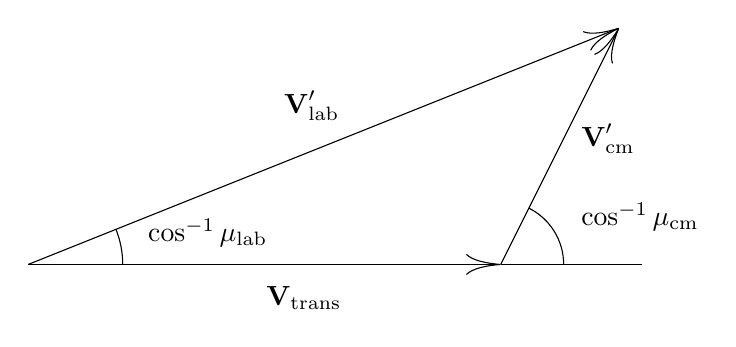
\begin{tikzpicture}
% the triangle
  \draw[-{>[scale=2.5,
          length=5,
          width=3]},line width=0.4pt] (0, 0) -- (7.5, 3);
  \draw[-{>[scale=2.5,
          length=5,
          width=3]},line width=0.4pt] (0, 0) -- (6, 0);
  \draw[-{>[scale=2.5,
          length=5,
          width=3]},line width=0.4pt] (6, 0) -- (7.5, 3);
 % \draw[->, stealth, line width=0.4pt] (6, 0) -- (7.5, 3);
\draw (6, 0) -- (7.8, 0);
  \draw ( 1.2, 0) arc (0: 21.8: 1.2);
  \draw (6.8, 0) arc (0: 63.43: 0.8);
% labels
  \node [below] at (3.5, -0.15) {$\Vtrans$};
  \node [above] at (3.6, 1.7) {$\Vlab'$};
  \node [right] at (6.9, 1.6) {$\Vcm'$};
  \node [right] at (1.4, 0.4) {$\cos^{-1} \mulab$};
  \node [right] at (6.9, 0.6){$\cos^{-1} \mucm$};
\end{tikzpicture}
\caption{Newtonian mapping to laboratory coordinates}
\label{Fig:2-body-boost}
\end{center} 

\end{figure}

It is also necessary to determine the direction cosine $\mulab$ in
the laboratory frame for
$$
     \Vtrans \cdot \Vlab' = \mulab \vtrans \vlab'.
$$
This is most easily derived from the trigonometry in Figure~\ref{Fig:2-body-boost}
$$
  \mulab  \vlab' = 
   \vtrans + \mucm \vcm'.
$$
In terms of the energies defined in Eqs.~(\ref{E_cm}), (\ref{E_trans}),
and~(\ref{E_lab}), this relation takes the form
\begin{equation}
  \mulab  = \frac
   { \sqrt{ \Etrans' } + \mucm \sqrt{ \Ecm'} }
    {\sqrt{\Elab'}}
    \quad \text{if $\Elab' > 0$.}
  \label{get_mu}
\end{equation}

It is clear from Eq.~(\ref{V-lab-2-body}) that 
$$
  \Elab' = \frac{\myo {\vlab'}^2}{2} = 0,
$$
if and only if
$$
  \Vcm' = - \Vtrans.
$$
In this case, the value of $\mulab$ is undefined.

\section{Computation of the transfer matrix from data for
discrete 2-body reactions}
Consider the use of data $g(\mucm \mid E)$ in Eq.~(\ref{prob_cm})
in the computation of integrals for the transfer matrix
Eqs.~(\ref{Inum}) and~(\ref{Ien}), either as tables or as Legendre
coefficients in Eq.~(\ref{cmLegendre}).  In these integrals
the multiplicity is always $M(E) = 1$ for discrete 2-body reactions.
The discussion given here concentrates on the
evaluation of the integral in Eq.~(\ref{Inum}).  The integral in
Eq.~(\ref{Ien}) differs only in that its integrand contains an extra
factor $\Elab'$, the energy of the outgoing particle in the laboratory frame.

Because the probability density data $g(\mucm \mid E)$ in 
Eq.~(\ref{prob_cm}) is given in center-of-mass coordinates, it is
desirable to transform the integrals Eqs.~(\ref{Inum})
to the center-of-mass frame.
The center-of-mass form of the integral Eq.~(\ref{Inum}) is
\begin{equation}
    \Inum_{g,h,\ell} =
   \int_{\calE_g}dE \, \sigma ( E ) w(E) \widetilde \phi_\ell(E) 
     \int_{\mucm} d\mucm  \,  g(\mucm \mid E)
     \int_{\Ecm'} d\Ecm' \, P_\ell( \mulab ) \,
        \delta(\Ecm' - \Psi(E) )
  \label{cmint}
\end{equation}
with $\Psi(E)$ as given by Eq.~(\ref{E_cm}).
The range of integration over $\mucm$ and $\Ecm'$ in
Eq.~(\ref{cmint})  is such that for fixed incident energy $E$ in $\calE_g$,
the energy $\Elab'$ of the outgoing particle given by Eq.~(\ref{E_lab}) lies
in~$\calE_h'$.

Integration of Eq.~(\ref{cmint})  with respect to $\Ecm'$ yields the result that
\begin{equation}
    \Inum_{g,h,\ell} =
     \int_{\calE_g} dE \, \sigma ( E ) w(E) \widetilde \phi_\ell(E) 
    \int_{\mucm} d\mucm  \,
     P_\ell( \mulab ) g(\mucm \mid E),
  \label{muEint}
\end{equation}
where it is understood that the direction cosine $\mulab$ in the laboratory
frame is calculated from Eq.~(\ref{get_mu}) and that the range of
integration over $\mucm$ is such that $E$ is in~$\calE_h'$.

The \gettransfer\ code steps through the data $g(\mucm \mid E)$
to compute contributions to the entries of the transfer matrix in
Eq.~(\ref{muEint}).
The case of tabular data with direct interpolation (Section~\ref{Sec:direct-interp}) is
illustrated in the laboratory frame in Figure~\ref{Fig:2-body-region-lab}.
This figure shows an integration region identified by an incident energy
bin~$\calE_g$ and an outgoing energy bin~$\calE_h'$.  The data
$g(\mucm \mid E)$ are given at incident energies $E_{k-1}$ and
$E_k$, such that the interval $E_{k-1} < E < E_k$ overlaps the
energy bin~$\calE_g$.  Furthermore, it is assumed that data entries
$g(\mucm \mid E)$ for $\mucm = \mucmjm$ and $\mucm = \mucm$ are
given at $E = E_{k-1} $ or at $E = E_k$ and that the table contains
no entries $g(\mucm \mid E_{k-1})$ or $g(\mucm \mid E_k)$ for 
$\mucmjm < \mucm < \mucm$.  Any missing data values 
$g(\mucmjm \mid E_{k-1})$ or $g(\mucmj \mid E_{k-1})$ or
$g(\mucmjm \mid E_k)$ or~$g(\mucmj \mid E_k)$ are computed
by interpolation with respect to~$\mucm$.  The integration region
in the laboratory frame
for the contribution of such a set of data to the integral $\Inum_{g,h,\ell}$
in Eq.~(\ref{cmint}) is the shaded area of Figure~\ref{Fig:2-body-region-lab}.  This region is
mapped to center-of-mass coordinates in Figure~\ref{Fig:2-body-region-cm}.

\begin{figure}
% hyperbolas mucm = const in the (E, E') plane
\begin{center}
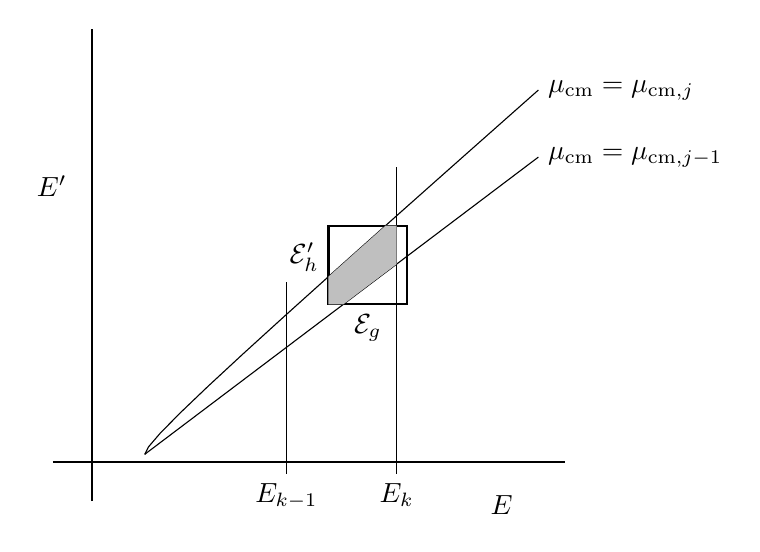
\begin{tikzpicture}
% the axes
  \draw[thick] (3.5,0) -- (10, 0);
  \draw[thick] (4,-0.5) -- (4, 5.5);
% the integration box
  \draw[thick](7,2) -- (7, 3) -- (8, 3) -- (8, 2) -- cycle;
% the data lines
  \draw (6.46667, -0.15) -- (6.46667, 2.28995);
  \node [below] at (6.46667, -0.15) {$E_{k-1}$};
  \draw (7.86667, -0.15) -- (7.86667, 3.74029);
  \node [below] at (7.86667, -0.15) {$E_{k}$};
% the curves
% mucm: -1
%\draw(4.66667, 0.0952381) --
%(4.71667, 0.0140642) --
%(4.86667, 0.00464791) --
%(5.11667, 0.0634261) --
%(5.46667, 0.187176) --
%(5.91667, 0.373109) --
%(6.46667, 0.618893) --
%(7.11667, 0.922636) --
%(7.86667, 1.28284) --
%(8.71667, 1.69832) --
%(9.66667, 2.16816);
% mucm: -0.5
%\draw(4.66667, 0.0952381) --
%(4.71667, 0.0735287) --
%(4.86667, 0.125453) --
%(5.11667, 0.24923) --
%(5.46667, 0.443248) --
%(5.91667, 0.706112) --
%(6.46667, 1.03666) --
%(7.11667, 1.43394) --
%(7.86667, 1.8972) --
%(8.71667, 2.42586) --
%(9.66667, 3.01946);
% mucm: 0
\draw(4.66667, 0.0952381) --
(9.66667, 3.87075);
% mucm: 0.5
\draw(4.66667, 0.0952381) --
(4.71667, 0.192458) --
(4.86667, 0.367064) --
(5.11667, 0.620838) --
(5.46667, 0.955391) --
(5.91667, 1.37212) --
(6.46667, 1.87219) --
(7.11667, 2.45654) --
(7.86667, 3.12593) --
(8.71667, 3.88094) --
(9.66667, 4.72204);
% mucm: 1
%\draw(4.66667, 0.0952381) --
%(4.71667, 0.251922) --
%(4.86667, 0.487869) --
%(5.11667, 0.806642) --
%(5.46667, 1.21146) --
%(5.91667, 1.70512) --
%(6.46667, 2.28995) --
%(7.11667, 2.96784) --
%(7.86667, 3.74029) --
%(8.71667, 4.60848) --
%(9.66667, 5.57333);
% integration region
\fill[gray!50] (7, 2) -- (7.0, 2.3517) -- 
(7.11667, 2.4565) -- (7.7256, 3) --
(7.86667, 3) -- (7.86667, 2.5116) --
(7.1892, 2) -- cycle;
% labels
 \node [below] at (9.2, -0.3) {$E$};
 \node [left] at (3.8, 3.5) {$E'$};
% \node [right] at (9.66667, 2.16816){$\mucm = -1$};
% \node [right] at (9.66667, 3.01946){$\mucm = -1/2$};
 \node [right] at (9.66667, 3.87075){$\mucm = \mucmjm$};
 \node [right] at (9.66667, 4.72204){$\mucm = \mucmj$};
% \node [right] at (9.66667, 5.57333){$\mucm = 1$};
 \node [left] at (7, 2.6){$\calE_h'$};
 \node [below] at  (7.5, 2){$\calE_g$};
\end{tikzpicture}
\caption{Integration region in the incident energy bin~$\calE_g$ and outgoing bin~$\calE_h'$
for probability data given at incident energies $E_{k-1}$ and~$E_k$ and direction
cosines $\mucmjm$ and~$\mucmj$ shown in the laboratory frame}
\label{Fig:2-body-region-lab}
\end{center} 

\end{figure}

\begin{figure}
% quadrature region in the (E, mucm) plane
\begin{center}
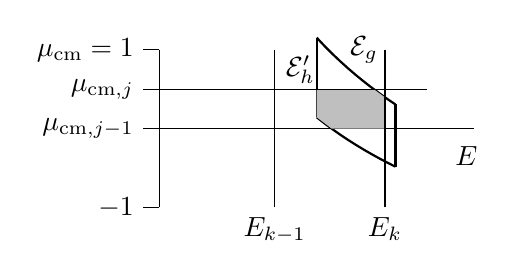
\begin{tikzpicture}
% the axes
  \draw (4.8,0) -- (9, 0);
  \draw (5,-1) -- (5, 1);
% the integration box
  \draw[thick] (7,0.1443) -- (7, 1.1547);
  \draw[thick] (8,-0.4841) -- (8, 0.3067);
% the curves
% Eout: 2
\draw[thick] (7, 0.144338) --
(7.1, 0.0661611) --
(7.2, -0.00780488) --
(7.3, -0.0779271) --
(7.4, -0.144528) --
(7.5, -0.207892) --
(7.6, -0.268272) --
(7.7, -0.325893) --
(7.8, -0.380958) --
(7.9, -0.433646) --
(8, -0.484123);
% Eout: 3
\draw[thick] (7, 1.1547) --
(7.1, 1.04855) --
(7.2, 0.948293) --
(7.3, 0.853396) --
(7.4, 0.763403) --
(7.5, 0.677908) --
(7.6, 0.596552) --
(7.7, 0.519015) --
(7.8, 0.445012) --
(7.9, 0.374288) --
(8, 0.306611);
% integration region
\fill[gray!50] (7, 0.1443) -- (7, 0.5) --
(7.7257, 0.5) -- (7.8, 0.445012) --
(7.86667, 0.3979) -- (7.86667, 0) --
(7.1894, 0) -- cycle;
% data lines
  \draw(4.8,0.5) -- (8.4, 0.5);
  \draw(6.46667, -1) -- (6.46667, 1);
  \node [below] at (6.46667, -1){$E_{k-1}$};
  \draw(7.86667, -1) -- (7.86667, 1);
  \node [below] at (7.86667, -1){$E_k$};
% labels
 \node [below] at (8.9, -0.1){$E$};
 \draw(4.8,-1) -- (5, -1);
 \node [left] at (4.8, -1){$-1$};
 \node [left] at (4.8, 0){$\mucmjm$};
 \node [left] at (4.8, 0.5){$\mucmj$};
  \draw(4.8,1) -- (5, 1);
 \node [left] at (4.8, 1){$\mucm = 1$};
 \node [left] at  (7.1, 0.75){$\calE_h'$};
 \node [above] at  (7.6, 0.7){$\calE_g$};
\end{tikzpicture}
\caption{Integration region of Fig.~\ref{Fig:2-body-region-lab} shown in center-of-mass coordinates}
\label{Fig:2-body-region-cm}
\end{center} 

\end{figure}

When the tabular data are interpolated by the method of cumulative
points of Section~\ref{Sec:cumProb}, the geometry is complicated by the
local unit-base transformations, but the basic ideas are the same.
Finally, for probability density data $g( \mucm \mid E)$ given as
Legendre coefficients in Eq.~(\ref{cmLegendre}), the only significant
difference is that the range of direction cosines becomes $-1 \le \mucm \le 1$
with the limitation that the energy $E$ of the outgoing particle lies in the
energy bin~$\calE_h'$.

\section{Format of data in the input file}
For tabulated probability density data $g( \mucm \mid E)$, the
data identifier as in Section~\ref{data-model}, is\\
  \Input{Process: two body transfer matrix}{}\\
and for the Legendre coefficients it is\\
  \Input{Process: Legendre two body transfer matrix}{}

\subsection{Data for both forms of probability density}
Because the boost from the center-of-mass frame to the laboratory
frame depends on the rest masses of the particles, these must be included
in the input file as described in Section~\ref{model-info}.  The format for doing so is\\
  \Input{Projectile's mass:}{$\myi$} \\
 \Input{Target's mass:}{$\mtarg$} \\
 \Input{Product's mass:}{$\myo$} \\
 \Input{Reaction's Q value:}{$Q$} \\
The values of these quantities must be in the same units as
the energy bin boundaries.

The code computes the rest mass of the residual from the $Q$ value and
the masses of the other particles.  If the input file also contains the line\\
 \Input{Residual's mass:}{$\mres$}\\
the code compares this value with the mass it computed, printing
a warning message if they are significantly different.

The code may use either Newtonian or relativistic mechanics in its
computations as specified in Section~\ref{Sec:relativistic}.

The specifications that the energy $E$ of the incident particle is given in the laboratory
frame and the direction cosine $\mucm$ in the center-of-mass frame are,
Section~\ref{Reference-frame},\\
  \Input{Projectile Frame:  lab}{}\\
  \Input{Product Frame:  CenterOfMass}{}

\subsection{Angular probability density tables}
The identification line for tabulated angular probability densities
is\\
  \Input{Angular data:}{$n = K$}\\
where $K$ is the number of incident energies~$E$.
This is followed by the interpolation rules for probability
densities from Section~\ref{interp-flags-probability}\\
  \Input{Incident energy interpolation:}{probability interpolation flag}\\
  \Input{Outgoing cosine interpolation:}{list interpolation flag}

There are then $K$ blocks, one for each incident energy $E_k$,\\
  \Input{Ein: $E_k$:}{$n = J_k$}\\
with $J_k$ pairs of values $\mucmj$ and $g(\mucm \mid E_k)$.  Thus,
with incident energy in MeV
a table of angular probability densities $g( \mucm \mid E)$ may look like\\
  \Input{Angular data:}{$n = 22$}\\
  \Input{Incident energy interpolation:}{lin-lin direct}\\
  \Input{Outgoing cosine interpolation:}{lin-lin}\\
  \Input{ Ein: 1.500000000000e-01 : n = 2}{}\\
   \Input{\indent -1.000000000000e+00  5.000000000000e-01}{}\\
    \Input{\indent 1.000000000000e+00  5.000000000000e-01}{}\\
  \Input{ Ein: 2.000000000000e-01 : n = 2}{}\\
  \Input{\indent  -1.000000000000e+00  4.550000000000e-01}{}\\
    \Input{\indent 1.000000000000e+00  5.450000000000e-01}{}\\
   \Input{\indent  } {$\cdots$}\\
  \Input{ Ein: 2.000000000000e+01 : n = 29}{}\\
   \Input{\indent -1.000000000000e+00  3.873180000000e-02}{}\\
  \Input{\indent  -9.500000000000e-01  2.943580000000e-02}{}\\
   \Input{\indent -9.000000000000e-01  2.582090000000e-02}{}\\
   \Input{\indent  } {$\cdots$}\\
    \Input{\indent 9.000000000000e-01  2.530490000000e+00}{}\\
   \Input{\indent 9.500000000000e-01  3.873180000000e+00}{}\\
    \Input{\indent 1.000000000000e+00  8.262750000000e+00}{}

\subsection{Legendre coefficients of angular probability density}
Legendre coefficient data of the form Eq.~(\ref{cmLegendre})
for discrete 2-body reactions are given as\\
    \Input{Legendre coefficients:}{$n = K$}\\
where $K$ is the number of incident energies~$E$.
This is followed by the interpolation rule for simple lists
from Section~\ref{interp-flags-list}\\
  \Input{Interpolation:}{list interpolation flag}

The file closes with $K$ sets of data\\
    \Input{Ein: $E_k$:}{$n = L_k$}\\
with $L_k$ Legendre coefficients $c_\ell(E_k)$ for $\ell = 0$, 1,
\ldots\ , $L_k - 1$ in Eq.~(\ref{cmLegendre}).  With incident energy
in units of MeV, an example of this portion of the input file is\\
   \Input{Legendre coefficients: n = 17}\\
  \Input{Interpolation:}{lin-lin}\\
  \Input{  Ein: 1.843100e+00:  n = 3}{}\\
    \Input{\indent 1.000000e+00}{}\\
    \Input{\indent 0.000000e+00}{}\\
    \Input{\indent 0.000000e+00}{}\\
   \Input{\indent  } {$\cdots$}\\
  \Input{ Ein: 2.000000e+01:  n = 12}{}\\
    \Input{\indent 1.000000e+00}{}\\
    \Input{\indent 4.640500e-01}{}\\
    \Input{\indent 2.320700e-01}{}\\
    \Input{\indent 8.593700e-02}{}\\
    \Input{\indent 5.338700e-02}{}\\
    \Input{\indent 2.465600e-02}{}\\
    \Input{\indent -1.500600e-03}{}\\
    \Input{\indent -1.756300e-02}{}\\
   \Input{\indent  -1.108000e-02}{}\\
    \Input{\indent 1.931100e-02}{}\\
    \Input{\indent 1.150900e-02}{}\\
    \Input{\indent 5.643500e-03}{}




\chapter{Isotropic energy probability densities in the laboratory frame}
\label{Sec:isotropic-lab}
The \xendl\ library supports several formats for energy probability densities
which are isotropic in the
laboratory frame.  These data are typically used for equilibrium
reactions and for fission neutrons.  Because the outgoing
distribution is isotropic, the probability density
$\pi(\Elab', \mulab   \mid E)$ in Eq.~(\ref{def_pi}) takes the form
\begin{equation}
  \pi(\Elab', \mulab   \mid E) = \pi_0(\Elab' \mid E).
 \label{isotropic-pi}
\end{equation}
Consequently, for the number-conserving
matrices only the $\ell = 0$ Legendre order,
\begin{equation}
   \Inum_{g,h,0} =
     \int_{\calE_g} dE \, \sigma ( E ) M(E) w(E) \widetilde \phi_0(E)
   \int_{\calE_h'} d\Elab' \, \pi_0(\Elab' \mid E)
 \label{InumI4-0}
\end{equation}
needs to be computed,
and Eq.~(\ref{Ien}) for the energy-preserving transfer matrix becomes
\begin{equation}
   \Ien_{g,h,0} =
     \int_{\calE_g} dE \, \sigma ( E ) M(E) w(E) \widetilde \phi_0(E) 
     \int_{\calE_h'} d\Elab' \, \pi_0(\Elab' \mid E) \Elab'.
 \label{IenI4-0}
\end{equation}

The data $\pi_0(\Elab' \mid E)$ may be given in \xendl\ either as
a table of values or as parameters in a function formula.
Because several of the function formulas for isotropic energy
probability densities are given in terms of incomplete gamma
functions, these are discussed first.  This is followed by a presentation
of the functional formulas for isotropic probability densities.  Then,
 the treatment of tables of~$\pi_0(\Elab' \mid E)$ for isotropic emission
 in the laboratory frame is discussed.  The section closes with
 the special treatment of the evaporation of delayed fission neutrons.

\section{Computational aspects of incomplete gamma functions}
Many
of the function formulas for $\pi_0(\Elab' \mid E)$ make use of the 
lower incomplete gamma function
\begin{equation}
  \gamma(\kappa, x) =
   \int_0^x dt\, t^{\kappa - 1} e^{-t}
  \label{def-gamma}
\end{equation}
with $\kappa > 0$.  The upper incomplete gamma
function is
\begin{equation}
  \Gamma(\kappa, x) =
   \int_x^\infty dt\, t^{\kappa - 1} e^{-t},
  \label{def-Gamma}
\end{equation}
and they are related by
$$
  \gamma(\kappa, x) + \Gamma(\kappa, x) = \Gamma(\kappa) =
  \int_0^\infty dt\, t^{\kappa - 1} e^{-t}.
$$
In order to reduce the difficulties of computer round-off,
the formula
$$
  \int_a^b dt\, t^{\kappa - 1} e^{-t} =
  \gamma( \kappa, b ) - \gamma( \kappa, a )
$$
is used when $0 \le a < b \le 1$, and
$$
  \int_a^b dt\, t^{\kappa - 1} e^{-t} =
  \Gamma( \kappa, a ) - \Gamma( \kappa, b )
$$
is used when $1 \le a < b$.  Either form may be used when
$a < 1 < b$.

Note that even though it is possible to write down
exact formulas for $\gamma(\kappa, x)$ when $\kappa$ is a
positive integer, it is better not to use them in the computations.
For example, it is true that
$$
  \gamma(2, x) = 1 - (1 + x)e^{-x}.
$$
For values of $x$ near zero, this formula involves subtracting
from 1 a number very close to 1 to get a result close to~$x^2/2$.
This is may lead to bad round-off errors in the computer arithmetic, 
and it is far better to
use the software for~$\gamma(2, x)$.

\section{Functional formulas for isotropic probability densities}
The functional formulas used in  \xendl\ for energy 
probability densities~$\pi_0(\Elab' \mid E)$ are the evaporation model,
the Maxwell model, the Watt model, and the Madland-Nix model.
These models are discussed in turn.  For all of these models the
energy of the outgoing particle is in the laboratory frame.

\subsection{Evaporation model}
For the evaporation model the formula is
\begin{equation}
  \pi_0(\Elab' \mid E) = C \Elab' \expon{- \frac{\Elab'}{\Theta(E)}}
 \label{evaporationF}
\end{equation}
with $0 \le \Elab' \le E - U$.  The value of $C$ in Eq.~(\ref{evaporationF})
is chosen so that
$$
  \int_0^{E - U} d\Elab' \, \pi_0(\Elab' \mid E) = 1.
$$
That is, 
$$
  C = \frac{1}{\Theta^2 \gamma(2, (E - U)/\Theta)}.
$$
The data consist of the energy of the reaction $U$ and pairs of
values $\{E, \Theta(E)\}$.  The 1-dimensional interpolation methods
of Section~\ref{Sec:1d-interp} are used to
determine the value of $\Theta$ for intermediate values of the 
energy $E$ of the incident particle.

According to the comment on incomplete gamma functions above,
for the calculation of $\Inum_{g,h,0}$ on an outgoing energy bin,
$E_0 \le \Elab' \le E_1$ the expression
$$
  \int_{E_0}^{E_1} d\Elab' \, \pi_0(\Elab' \mid E) =
   C\Theta^2[\gamma(2, E_1/\Theta) - \gamma(2, E_0/\Theta)]
$$
is used when $E_0 \le \Theta$, and
$$
  \int_{E_0}^{E_1} d\Elab' \, \pi_0(\Elab' \mid E) =
   C\Theta^2[\Gamma(2, E_0/\Theta) - \Gamma(2, E_1/\Theta)]
$$
is used when $E_0 > \Theta$.  Analogously, for the
calculation of $\Ien_{g,h,0}$
$$
  \int_{E_0}^{E_1} d\Elab' \, \Elab' \pi_0(\Elab' \mid E) =
   C\Theta^3[\gamma(3, E_1/\Theta) - \gamma(3, E_0/ \Theta)]
$$
is used when $E_0 \le \Theta$, and
$$
  \int_{E_0}^{E_1} d\Elab' \, \Elab' \pi_0(\Elab'  \mid E) =
   C\Theta^3[\Gamma(3, E_0/\Theta) - \Gamma(3, E_1/\Theta)]
$$
is used otherwise.

\subsubsection{Input file data for the evaporation model}
The process identifier in Section~\ref{data-model} is\\
  \Input{Process: evaporation spectrum}{}\\
These data are always in the laboratory frame,\\
  \Input{Product Frame: lab}{}

One item of model-dependent data in Section~\ref{model-info}
is the value of $U$ used in defining the range of outgoing
energies $E$ in Eq.~(\ref{evaporationF}), and it is given by\\
  \Input{U:}{$U$}\\
The other input data are the values of $\Theta(E)$ in
Eq.~(\ref{evaporationF}) depending on the incident energy~$E$.  
All of these energies, $U$, $E$, and $\Theta(E)$, must be in the same
units as the energy bins in Sections~\ref{Ein-bins} and~\ref{Eout-bins}.
The format for these data is\\
  \Input{Theta: n = $n$}{}\\
  \Input{Interpolation:}{interpolation flag}\\
with $n$ pairs of entries $\{E, \Theta(E)\}$.  
The interpolation flag is one of those for simple lists as in 
Section~\ref{interp-flags-list}.
For example, in units of MeV one may have\\
  \Input{U: 11.6890}{}\\
  \Input{Theta: n = 2}{}\\
  \Input{Interpolation: lin-lin}{}\\
  \Input{ 12.0 1.04135}{}\\
  \Input{ 20.0 1.04135}{}

\subsection{Maxwell model}
The formula for the Maxwell is
\begin{equation}
  \pi_0(\Elab'  \mid E) = C \sqrt{\Elab' } \, \expon{- \frac{\Elab' }{\Theta(E)}}
 \label{MaxwellF}
\end{equation}
for $0 \le \Elab'  \le E - U$.  This model is often used for fission neutrons.
The value of $C$ in Eq.~(\ref{MaxwellF}) is given by
$$
  C = \frac{1}{\Theta^{3/2} \gamma(3/2, (E - U)/\Theta)}.
$$
Because of round-off problems with small values of $x$,
it is unwise to use the mathematically equivalent formula
$$
  \gamma(3/2, x) =
  \frac{\sqrt{\pi}}{2}\, \erf{\sqrt{x}} - \sqrt{x}\,e^{-x}.
$$
The data consist of the energy of the reaction $U$ and pairs of
values $\{E, \Theta(E)\}$.  The parameter $\Theta$ is interpolated
by the methods of Section~\ref{Sec:1d-interp} to obtain intermediate values. 

Depending on the value of $E_0/\Theta$,
the calculation of $\Inum_{g,h,0}$ on an outgoing energy bin
$E_0 \le \Elab'  \le E_1$ uses the expression
$$
  \int_{E_0}^{E_1} d\Elab'  \, \pi_0(\Elab'  \mid E) =
   C\Theta^{3/2}[\gamma({3/2}, E_1/\Theta) - \gamma({3/2}, E_0/\Theta)]
$$
or
$$
  \int_{E_0}^{E_1} d\Elab'  \, \pi_0(\Elab'  \mid E) =
   C\Theta^{3/2}[\Gamma({3/2}, E_0/\Theta) - \Gamma({3/2}, E_1/\Theta)].
$$
Analogously, the calculation of $\Ien_{g,h,0}$ uses either
$$
  \int_{E_0}^{E_1} d\Elab'  \, \Elab' \pi_0(\Elab'  \mid E) =
   C\Theta^{5/2}[\gamma({5/2}, E_1/\Theta) - \gamma({5/2}, E_0/\Theta)]
$$
or
$$
  \int_{E_0}^{E_1} d\Elab'  \, \Elab' \pi_0(\Elab'  \mid E) =
   C\Theta^{5/2}[\Gamma({5/2}, E_0/\Theta) - \Gamma({5/2}, E_1/\Theta)].
$$

\subsubsection{Input file data for the Maxwell model}
The process identifier in Section~\ref{data-model} is\\
  \Input{Process: Maxwell spectrum}{}\\
Again, this data is in the laboratory frame,\\
  \Input{Product Frame: lab}{}

One item of model-dependent data in Section~\ref{model-info}
is the value of $U$ used in defining the range of outgoing
energies $E$ in Eq.~(\ref{MaxwellF}), and it is given by\\
  \Input{U:}{$U$}\\
The other input data are the values of $\Theta(E)$ in
Eq.~(\ref{MaxwellF}) depending on the incident energy~$E$.  
These energies, $U$, $E$, and $\Theta(E)$, must all be in the same
units as the energy bins in Sections~\ref{Ein-bins} and~\ref{Eout-bins}.
The format for such data is\\
  \Input{Theta: n = $n$}{}\\
  \Input{Interpolation:}{interpolation flag}\\
with $n$ pairs of entries $\{E, \Theta(E)\}$.  
The interpolation flag is one of those for simple lists as in 
Section~\ref{interp-flags-list}.
For example, in units of MeV one may have\\
  \Input{U: -20}{}\\
  \Input{Theta: n = 2}{}\\
  \Input{Interpolation: lin-lin}{}\\
  \Input{ 1.0e-11  1.28}{}\\
  \Input{ 20.0  1.28}{}

\subsection{Watt model}
Another model sometimes used for fission neutrons in \xendl\ is the Watt
formula
\begin{equation}
  \pi_0(\Elab'  \mid E) = C \sinh{\sqrt{b\Elab' }}\, \expon{- \frac{\Elab' }{a}}
 \label{WattF}
\end{equation}
for $0 \le \Elab'  \le E - U$.
The value of $C$ in Eq.~(\ref{WattF})
is given by
$$
  \frac{1}{C} =
  \frac{az\sqrt{\pi}}{2}\, \expon{z^2}
  \left(
    \erf{y - z} - \erf{y + z}
  \right) -
  a \expon{-y^2} \sinh{\sqrt{b(E - U)}}
$$
with $y = \sqrt{(E - U)/a}$ and $z = \sqrt{ab /4}$.
The data consist of the energy of the reaction $U$ and pairs of
values $\{E, a(E)\}$ and $\{E, b(E)\}$.  For intermediate incident
energies $E$, the parameters $b$ and~$a$ are interpolated by
the methods of Section~\ref{Sec:1d-interp}.

\subsubsection{Input file data for the Watt model}
The process identifier in Section~\ref{data-model} is\\
  \Input{Process: Watt spectrum}{}\\
This data is in the laboratory frame,\\
  \Input{Product Frame: lab}{}

One item of model-dependent data in Section~\ref{model-info}
is the value of $U$ used in defining the range of outgoing
energies $E$ in Eq.~(\ref{WattF}), and it is given by\\
  \Input{U:}{$U$}\\
The other input data are the values of $a(E)$ and $b(E)$ in
Eq.~(\ref{WattF}).  
The energies, $U$, $E$, and $a(E)$, must be in the same
units as the energy bins in Sections~\ref{Ein-bins} and~\ref{Eout-bins},
and the units for $b(E)$ are the reciprocal of these units.
The format for these data is\\
  \Input{a: n = $n$}{}\\
  \Input{Interpolation:}{interpolation flag}\\
with $n$ pairs of entries $\{E, a(E)\}$ and\\
  \Input{b: n = $n$}{}\\
  \Input{Interpolation:}{interpolation flag}\\
with $n$ pairs of entries $\{E, b(E)\}$.
The interpolation flags for $a$ and $b$ are those for simple lists as in 
Section~\ref{interp-flags-list}.
For example, with energies in MeV  one may have\\
  \Input{U: -10}{}\\
  \Input{a: n = 11}{}\\
  \Input{Interpolation: lin-lin}{}\\
  \Input{ 1.000000e-11    9.770000e-01}{}\\
  \Input{ 1.500000e+00   9.770000e-01}{}\\
  \Input{}{ $\cdots$}\\
     \Input{ 3.000000e+01 1.060000e+00}{}\\
  \Input{b: n = 11}{}\\
  \Input{Interpolation: lin-lin}{}\\
  \Input{ 1.000000e-11    2.546000e+00}{}\\
  \Input{ 1.500000e+00   2.546000e+00}{}\\
  \Input{}{ $\cdots$}\\
     \Input{ 3.000000e+01 2.620000e+00}{}

\subsection{Madland-Nix model}\label{Sec:Madland}

The Madland-Nix model~\cite{Madland} for prompt fission neutrons uses 
the formula
\begin{equation}
  \pi_0(\Elab'  \mid E) = \frac{C}{2}\, [g(\Elab' , E_{FL}) + g(\Elab' , E_{FH})]
 \label{Madland-NixF}
\end{equation}
for
\begin{equation}
 0 \le \Elab' \le \texttt{maxEout},
 \label{Madland-Nix-E-range}
\end{equation}
where \texttt{maxEout} is one of the input parameters.
Note that the range of outgoing energies Eq.~(\ref{Madland-Nix-E-range})
is independent of the incident energy.
In fact, the \ENDF\ manual~\cite{ENDFB} gives no way for the data to specify the
maximum outgoing energy for the Madland-Nix model. 

In Eq.~(\ref{Madland-NixF}) $E_{FL}$ is the average kinetic energy of the light fission
fragments, and $E_{FH}$ is the average kinetic energy of the heavy fission
fragments.  The function $g(\Elab' , E_F)$ in Eq.~(\ref{Madland-NixF}) is given in terms
of the parameters $T_m$ and
\begin{equation}
   u_1 = \frac{(\sqrt{\Elab' } - \sqrt{E_F})^2}{T_m}, \quad
   u_2 = \frac{(\sqrt{\Elab' } + \sqrt{E_F})^2}{T_m}
 \label{Madland-Nixu}
\end{equation}
by the formula
\begin{equation}
   g(\Elab' , E_F) = \frac{1}{3\sqrt{E_F T_m}}
   \left[
     u_2^{3/2}E_1(u_2) - u_1^{3/2}E_1(u_1) -
     \Gamma(3/2, u_2) + \Gamma(3/2, u_1)
   \right],
 \label{Madland-Nixg}
\end{equation}
where $E_1$ denotes the exponential integral
$$
  E_1(x) = \int_x^\infty dt\, \frac{1}{t}e^{-t}.
$$
It is clear from the definitions that
$$
  E_1(x) = \Gamma(0, x),
$$
but software to compute $\Gamma(\kappa, x)$ generally requires
that $\kappa$ be positive.
The data for the Madland-Nix model contains the average energies
$E_{FL}$ and $E_{FH}$ as well as pairs of values $\{E, T_m(E)\}$.
The interpolation rule for $T_m$ is also given.

If the range of outgoing energies is taken to be $0 \le \Elab'  < \infty$ 
in Eq.~(\ref{Madland-NixF}), then $C = 1$.  For other ranges of $\Elab' $
and for computation of $\Inum_{g,h,0}$, it follows from Eq.~(\ref{Madland-Nixg})
that it is necessary to compute integrals
\begin{equation}
 \calG_i( a, b ) =  \int_a^b d\Elab'  \, u_i^{3/2}E_1(u_i)
 \label{Madland-Nix-u-integral}
\end{equation}
and
\begin{equation}
 \calH_i( a, b ) =   \int_a^b d\Elab'  \, \Gamma(3/2, u_i)
 \label{Madland-Nix-Gamma-integral}
\end{equation}
with $i = 1$, 2.

The values of the integrals Eqs.~(\ref{Madland-Nix-u-integral})
and~(\ref{Madland-Nix-Gamma-integral}) are conveniently expressed
in terms of the parameters
\begin{equation}
  \alpha = \sqrt{T_m}, \quad
  \beta = \sqrt{E_F},
 \label{Madland-Nix-alpha-beta}
\end{equation}
\begin{equation}
  A = \frac{(\sqrt{a} + \beta)^2}{\alpha^2}, \quad
  B = \frac{(\sqrt{b} + \beta)^2}{\alpha^2},
 \label{Madland-Nix-A-B}
\end{equation}
and
\begin{equation}
  A' = \frac{( \beta - \sqrt{a})^2}{\alpha^2}, \quad
  B' = \frac{(\sqrt{b} - \beta)^2}{\alpha^2}.
 \label{Madland-Nix-A-B-prime}
\end{equation}

One might think it sufficient to calculate
$$
  \calG_i( 0, b )  \quad \text{and} \quad
  \calH_i( 0, b ) 
$$
in Eqs.~(\ref{Madland-Nix-u-integral}) and~(\ref{Madland-Nix-Gamma-integral})
and to use
\begin{equation*}
 \begin{split}
   \calG_i( a, b ) &= \calG_i( 0, b ) - \calG_i( 0, a ), \\
   \calH_i( a, b ) &= \calH_i( 0, b ) - \calH_i( 0, a )
 \end{split}
\end{equation*}
for $i = 1$, 2.  In fact, this approach is suitable only for $i = 2$.
The reason for the difficulty is seen from Eqs.~(\ref{Madland-Nixu})
and~(\ref{Madland-Nix-alpha-beta}), in that
\begin{equation}
  u_1^{3/2} = \begin{cases}
    (\beta - \sqrt{\Elab' })^3 / \alpha^3  \quad &\text{for $0 \le \Elab'  \le \beta^2$}, \\
    (\sqrt{\Elab' } - \beta)^3 / \alpha^3 \quad &\text{for $\Elab'  > \beta^2$}.
    \end{cases}
 \label{Madland-Nix-u1}
\end{equation}

Consequently, the integrals used to compute $\calG_i( a, b )$
and~$\calH_i( a, b )$ in Eqs.~(\ref{Madland-Nix-u-integral}) 
and (\ref{Madland-Nix-Gamma-integral}) are evaluated as
\begin{equation}
  \calG_1( a, \beta^2 ) = 
    \frac{\alpha \beta}{2} \, \gamma \left( 2, A' \right)
       -\frac{2 \alpha^2}{5} \, \gamma \left( \frac{5}{2}, A' \right) +
       \left[
          \frac{2 \alpha \sqrt{A'}}{5} - \frac{\beta}{2}
        \right] \alpha {A'}^2 E_1( A' )
       \quad \text{for $0 \le a < \beta^2$},
\label{Madland-Nix-G1a}
\end{equation}
\begin{equation}
  \calG_1( \beta^2, b ) = 
    \frac{\alpha \beta}{2} \, \gamma \left( 2, B' \right)
       + \frac{2 \alpha^2}{5} \, \gamma \left( \frac{5}{2}, B' \right) +
       \left[
          \frac{\beta}{2} + \frac{2 \alpha \sqrt{B'}}{5}
        \right] \alpha {B'}^2 E_1( B' )
       \quad \text{for $b > \beta^2$},
 \label{Madland-Nix-G1b}
\end{equation}
\begin{equation}
 \begin{split}
  \calG_2( 0, b )  = &
    \frac{2 \alpha^2}{5} \, \gamma \left( \frac{5}{2}, B \right) -
    \frac{\alpha \beta}{2} \, \gamma \left( 2, B \right) -
    \frac{\beta^5}{10 \alpha^3} \,e^{-B} + {}\\
      & \left[
        \frac{2 \alpha^2}{5} B^{5/2} - \frac{\alpha \beta}{2} {B}^2 +
          \frac{ \beta^5}{10 \alpha^3} \right]  E_1( B) - C_1
       \quad \text{for $b \ge 0$},
 \end{split}
\label{Madland-Nix-G2}
\end{equation}
\begin{equation}
  \calH_1(a, \beta^2) = 2 \alpha \beta \, \gamma \left( 2, A' \right) -
  \alpha^2 \, \gamma \left( \frac{5}{2}, A' \right) +
     (\beta^2 - a) \, \Gamma\left( \frac{3}{2}, A' \right)
     \quad \text{for $0 \le a < \beta^2$},
\label{Madland-Nix-H1a}
\end{equation}
\begin{equation}
  \calH_1(\beta^2, b) = 2 \alpha \beta \, \gamma \left( 2, B' \right) +
     \alpha^2 \, \gamma \left( \frac{5}{2}, B' \right) +
     (b - \beta^2) \, \Gamma\left( \frac{3}{2}, B' \right)
     \quad \text{for $b \ge \beta^2$},
\label{Madland-Nix-H1b}
\end{equation}
and
\begin{equation}
   \calH_2(0, b) = \alpha^2 \, \gamma \left( \frac{5}{2}, B \right) -
     2 \alpha\beta \, \gamma \left( 2, B \right) +
     \beta^2 \, \gamma \left( \frac{3}{2}, B \right) +
     b \, \Gamma \left( \frac{3}{2}, B \right) - C_2
     \quad \text{for $b > 0$}.
\label{Madland-Nix-H2}
\end{equation}
In the relations for $\calG_2(0, b)$ and $\calH_2(0, b)$ above, $C_1$
and~$C_2$ are constants of integration.

\begin{figure}
% domain of integration for the Madland-Nix model
\begin{center}
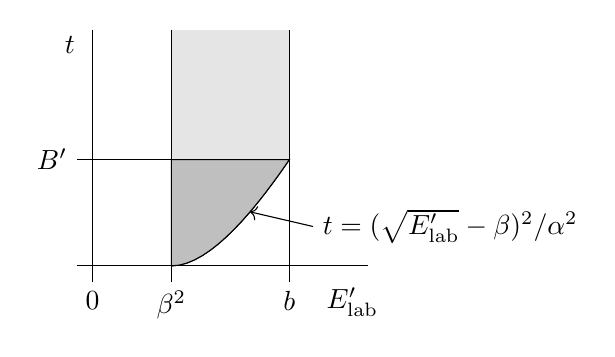
\begin{tikzpicture}
% the u_1(E) curve
\draw( 1.0 , 0.0 ) --
( 1.1 , 0.00952921463879 ) --
( 1.2 , 0.0364390799173 ) --
( 1.3 , 0.0785965992069 ) --
( 1.4 , 0.134272347041 ) --
( 1.5 , 0.202041028867 ) --
( 1.6 , 0.280711487461 ) --
( 1.7 , 0.369276151676 ) --
( 1.8 , 0.466873708001 ) --
( 1.9 , 0.572760998328 ) --
( 2.0 , 0.686291501015 ) --
( 2.1 , 0.806898603048 ) --
( 2.2 , 0.934082420647 ) --
( 2.3 , 1.06739928952 ) --
( 2.4 , 1.20645329214 ) --
( 2.5 , 1.35088935933 );
% integration regions
\filldraw[fill = gray!50]
( 1.0 , 0.0 ) --
( 1.1 , 0.00952921463879 ) --
( 1.2 , 0.0364390799173 ) --
( 1.3 , 0.0785965992069 ) --
( 1.4 , 0.134272347041 ) --
( 1.5 , 0.202041028867 ) --
( 1.6 , 0.280711487461 ) --
( 1.7 , 0.369276151676 ) --
( 1.8 , 0.466873708001 ) --
( 1.9 , 0.572760998328 ) --
( 2.0 , 0.686291501015 ) --
( 2.1 , 0.806898603048 ) --
( 2.2 , 0.934082420647 ) --
( 2.3 , 1.06739928952 ) --
( 2.4 , 1.20645329214 ) --
( 2.5 , 1.35088935933 ) --
(1, 1.35088935933 ) -- cycle;
\fill[ gray!20] ( 2.5 , 1.35088935933 ) --
(2.5, 3) -- (1, 3) --
( 1 , 1.35088935933 ) -- cycle;
% the axes and quadrature strip
 \draw(-0.2, 0) -- (3.5, 0);
 \draw(0, -0.2) -- (0, 3);
 \draw(-0.2, 1.35088935933) -- (2.5, 1.35088935933);
 \draw(1, -0.2) -- (1, 3);
 \draw(2.5, -0.2) -- (2.5, 3);
% labels
  \node [below] at (0, -0.2){0};
  \node [below] at (1, -0.2){$\beta^2$};
  \node [below] at (2.5, -0.2){$b$};
  \node [below] at (3.3, -0.15){$\Elab'$};
  \node [left] at (-0.2, 1.35){$B'$};
  \node [left] at (-0.1, 2.8){$t$};
  %legend
  \draw [<-] ( 2.0 , 0.686291501015 ) -- (2.8, 0.5);
  \node [right] at (2.8, 0.5) {$ t = (\sqrt{\Elab'} - \beta)^2/\alpha^2$};
\end{tikzpicture}
\caption{Domain of integration for $\calG_1( \beta^2, b )$ with $b > \beta^2$
in the Madland-Nix model}
\label{Fig:Madland-Nix}
\end{center} 

\end{figure}

In order to illustrate how the above integration formulas may be 
derived, consider the case of Eq.~(\ref{Madland-Nix-G1b})
for $\calG_1( \beta^2, b )$ defined in 
Eq.~(\ref{Madland-Nix-u-integral}) with $u_1$ as in
Eq.~(\ref{Madland-Nix-u1}) and with~$b > \beta^2$.  Substitution
of the definition of the exponential integral~$E_1$ gives the double
integral
$$
   \calG_1( \beta^2, b ) = \int_{\beta^2}^b d\Elab'  \,
      u_1^{3/2} \int_{u_1}^\infty dt \, \frac{1}{t} \, e^{-t}.
$$
The region of integration for this integral is the union of the
two shaded domains in Figure~\ref{Fig:Madland-Nix}.
The integral over the darker shaded region of Figure~\ref{Fig:Madland-Nix} is
$$
  J_{11} = \int_{\beta^2}^b d\Elab'  \, u_1^{3/2}\int_{u_1}^{B'} dt\, \frac { e^{-t}}{t}.
$$
Reversal of the order of integration transforms this integral to
$$
  J_{11} = \int_0^{B'} dt\, \frac{1}{t} \,e^{-t}
    \int_{\beta^2}^{(\alpha\sqrt{t} + \beta)^2}
       d\Elab' \, u_1^{3/2}.
$$
Under the substitution
\begin{equation*}
  \Elab'  = (\alpha \sqrt{u_1} + \beta)^2,
%  \label{u_for_E}
\end{equation*}
the inner integral takes the form
$$
  \int_{\beta^2}^{(\alpha\sqrt{t} + \beta)^2}
       d\Elab' \, u_1^{3/2} =
   \int_0^t du_1 \, u_1^{3/2}\left( 
       \alpha^2 + \frac{\alpha\beta}{\sqrt{u_1}} 
  \right) =
    \frac{2\alpha^2}{5}t^{5/2} + \frac{\alpha\beta}{2}t^2.
$$
Thus, it follows that the integral over the dark shaded region in
Figure~\ref{Fig:Madland-Nix} is
\begin{equation*}
  J_{11} = 
    \frac{2\alpha^2}{5} \, \gamma(5/2, B') + \frac{ \alpha\beta}{2} \, \gamma(2, B').
%  \label{intJ11}
\end{equation*}
This relation gives the first two terms on the right-hand side
of Eq.~(\ref{Madland-Nix-G1b}).

The other terms on the right-hand side of Eq.~(\ref{Madland-Nix-G1b})
result from evaluation of the integral over the light shaded region in
Figure~\ref{Fig:Madland-Nix},
$$
J_{12} = \int_{\beta^2}^b d\Elab'  \, u_1^{3/2} \int_{B'}^\infty dt\, \frac {e^{-t}}{t}
 = \int_{B'}^\infty dt\, \frac{1}{t} \, e^{-t}
    \int_{\beta^2}^{b}
       d\Elab' \, u_1^{3/2}.
$$  

\subsubsection{Input file data for the Madland-Nix model}
The process identifier in Section~\ref{data-model} is\\
  \Input{Process: Madland-Nix spectrum}{}\\
This data is in the laboratory frame,\\
  \Input{Product Frame: lab}{}

The model-dependent data in Section~\ref{model-info}
contains values of $E_{FL}$, the average kinetic energy of the
light fission fragment and $E_{FH}$, the average kinetic energy of the
heavy fission fragment.  These parameters are given by\\
  \Input{EFL:}{$E_{FL}$}\\
  \Input{EFH:}{$E_{FH}$}\\
The user must also specify a maximum outgoing energy 
\texttt{maxEout} for use in Eq.~(\ref{Madland-Nix-E-range}).
 
The other input data are the values of $T_m$ as a function of
incident energy in
Eq.~(\ref{Madland-NixF}).  The format for these data is\\
  \Input{TM: n = $n$}{}\\
  \Input{Interpolation:}{interpolation flag}\\
with $n$ pairs of entries $\{E, T_m(E)\}$.  
The interpolation flag is one of those for simple lists as in 
Section~\ref{interp-flags-list}.
The energies, $E_{FL}$, $E_{FH}$, $E$, and $T_m(E)$, must be in the same
units as the energy bins in Sections~\ref{Ein-bins} and~\ref{Eout-bins}.
For example, in MeV units one may have\\
  \Input{EFL: 1.029979}{}\\
  \Input{EFH: 0.5467297}{}\\
  \Input{maxEout: 60}{}\\
  \Input{TM: n = 38}{}\\
  \Input{Interpolation: lin-lin}{}\\
  \Input{ 1.0000000e-11   1.0920640e+00}{}\\
  \Input{ 5.0000010e-01  1.1014830e+00}{}\\
  \Input{}{ $\cdots$}\\
  \Input{ 2.0000000e+01  1.1292690e+00}{}

\section{Energy probability density tables}\label{Sec:isotropicTables}
Another form of isotropic probability density data $\pi_0(\Elab'  \mid E)$
Eq.~(\ref{isotropic-pi}) in \xendl\ is in the form of tables.  The computation
of transfer matrices for such data given in the laboratory frame is
discussed here.  For data in the center-of-mass frame, this is a
special case of Legendre expansions discussed in Section~\ref{Ch:Legendre-cm}
with Legendre order zero.
For given
incident energies $E_i$, the data consist of pairs 
$\{E_{k,j}', \pi_0(E_{k,j}' \mid E_k)\}$ as in Eq.~(\ref{EPtable}).
For such tabular data,
computation of the integrals $\Inum_{g,h,0}$ in Eq.~(\ref{InumI4-0})
and $\Ien_{g,h,0}$ in Eq.~(\ref{IenI4-0}) depends on the type
of interpolation used between
different incident energies.
The effects of the unit-base map Eq.~(\ref{unit-base-map}) are
discussed here.  The considerations are the same, whether the
unit-base map is used alone or as a component of interpolation
by cumulative points.

After the unit-base transformation Eq.~(\ref{unit-base-map})
the integrals Eqs.~(\ref{InumI4-0}) and~(\ref{IenI4-0}) take the form
\begin{equation}
   \Inum_{g,h,0} =
     \int_{\calE_g} dE \, \sigma ( E ) M(E) w(E) \widetilde \phi_0(E) 
   \int_{\widehat\calE_h'} d\widehat \Elab'  \,
     \widehat\pi_0(\widehat \Elab'   \mid E)
 \label{InumhatI4-0}
\end{equation}
and
\begin{equation}
   \Ien_{g,h,0} =
     \int_{\calE_g} dE \, \sigma ( E ) M(E) w(E) \widetilde \phi_0(E) 
   \int_{\widehat\calE_h'} d\widehat \Elab'   \,
     \widehat\pi_0(\widehat \Elab'   \mid E) \Elab'  .
 \label{IenhatI4-0}
\end{equation}
In these intergrals $\widehat\calE_h'$ denotes result of mapping the 
outgoing energy bin $\calE_h'$ with the transformation Eq.~(\ref{unit-base-map}).
Furthermore, $\Elab'  $ in Eq.~(\ref{IenhatI4-0}) is to be obtained from $\widehat \Elab'  $
using the inverse unit-base mapping Eq.~(\ref{unitbaseInvert}).

\begin{figure}
% domain of integration for energy probability density tables
\begin{center}
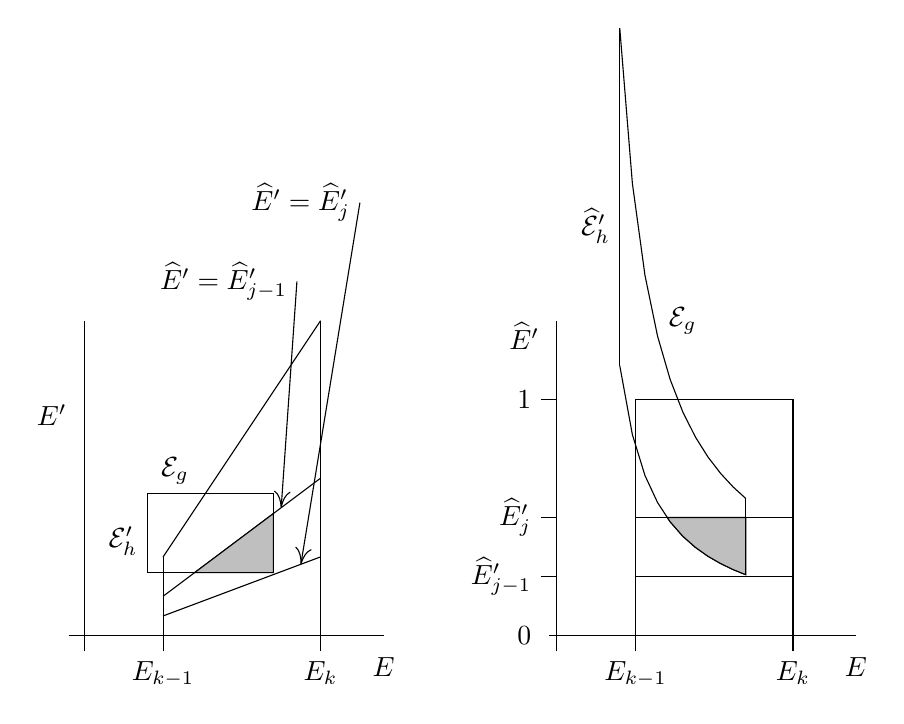
\begin{tikzpicture}
% the axes and quadrature strip
% the axes
  \draw(-0.2,0) -- (3.8, 0);
  \draw(0,-0.2) -- (0, 4);
  \node [below] at (3.8, -0.15){$E$};
  \node [left] at (-0.1, 2.8){$E'$};
% the E' lines
  \draw(1,-0.2) -- (1, 1);
  \draw(3,-0.2) -- (3, 4);
% integration box
  \draw(0.8, 0.8) -- (0.8, 1.8) --
  (2.4, 1.8) --
  (2.4, 0.8) -- cycle;
% labels
  \node [below] at (1, -0.2){$E_{k-1}$};
  \node [below]  at (3, -0.2){$E_{k}$};
  \node [left] at (0.8, 1.2){$\calE_h'$};
  \node [above] at (1.15, 1.8){$\calE_g$};
% the curves
  \draw(1,0.25) -- (3,1);
  \draw (1, 0.5) -- (3, 2);
  \draw (1, 1) -- (3, 4);
% integration region
\filldraw[fill = gray!50]
  (2.4, 0.8) -- (2.4, 1.55) -- (1.4, 0.8) -- cycle;
%%% the mapped picture
% the axes
  \draw(5.9,0) -- (9.8, 0);
  \draw(6,-0.2) -- (6, 4);
  \node [below] at(9.8, -0.15){$E$};
  \node [left] at(5.9, 3.8){$\widehat E'$};
  \draw(5.8,3) -- (6, 3);
  \node [left] at(5.8, 3){$1$};
  \node [left] at(5.8, 0){$0$};
  \draw(5.8,0.75) -- (6, 0.75);
  \node [left] at (5.8, 0.75){$\widehat E_{j-1}'$};
  \draw(5.8,1.5) -- (6, 1.5);
  \node [left] at (5.8, 1.5){$\widehat E_{j}'$};
% the E' lines
  \draw(7,-0.2) -- (7, 3);
  \draw(9,-0.2) -- (9, 3);
% the Ehat lines
  \draw(7, 0.75) -- (9, 0.75);
  \draw(7, 1.5) -- (9, 1.5);
  \draw(7, 3) -- (9, 3);
% integration box
  \draw(6.8, 3.4286) -- (6.8, 7.7143);
  \draw(8.4, 0.7743) -- (8.4, 1.74194);
% Eout: 0.8
\draw(6.8, 3.42857) --
(6.96, 2.55319) --
(7.12, 2.0339) --
(7.28, 1.69014) --
(7.44, 1.44578) --
(7.6, 1.26316) --
(7.76, 1.1215) --
(7.92, 1.0084) --
(8.08, 0.916031) --
(8.24, 0.839161) --
(8.4, 0.774194);
% Eout: 1.8
\draw(6.8, 7.71429) --
(6.96, 5.74468) --
(7.12, 4.57627) --
(7.28, 3.80282) --
(7.44, 3.25301) --
(7.6, 2.84211) --
(7.76, 2.52336) --
(7.92, 2.26891) --
(8.08, 2.06107) --
(8.24, 1.88811) --
(8.4, 1.74194);
% integration region
\filldraw[fill = gray!50]
  (8.4, 0.774194) -- (8.4, 1.5) --
  (7.4045, 1.5) -- (7.44, 1.44578) --
(7.6, 1.26316) --
(7.76, 1.1215) --
(7.92, 1.0084) --
(8.08, 0.916031) --
(8.24, 0.839161) -- cycle;
% labels
  \node [below] at (7, -0.2){$E_{k-1}$};
  \node [below] at (9, -0.2){$E_k$};
  \node [left] at (6.8, 5.2){$\widehat \calE_h'$};
  \node [right] at (7.3, 4){$\calE_g$};
%legend
\draw [{<[scale=2, length=3, width=3]}-] (2.75, 0.9063) -- (3.5, 5.5);
\node [left] at (3.5, 5.5) {$\widehat E' = \widehat E_j'$};
\draw [{<[scale=2, length=3, width=3]}-] (2.5, 1.625) -- (2.7, 4.5);
\node [left] at (2.7, 4.5) {$\widehat E' = \widehat E_{j-1}'$};
\end{tikzpicture}
\caption{Domains of integration for tabulated probability densities, laboratory
frame on the left and unit base on the right}
\label{Fig:unit-base-region}
\end{center} 

\end{figure}

Figure~\ref{Fig:unit-base-region} illustrates the effect of
the unit-base map Eq.~(\ref{unit-base-map}).   
For incident energies $E = E_{k-1}$ and~$E = E_k$,  
1-dimensional interpolation is used
to produce data at a common set of unit-base outgoing energies
$\{\widehat E_j'\}$. In the left-hand
portion of Figure~\ref{Fig:unit-base-region}, suppose that
probability densities $\pi_0(\Elab'   \mid E)$ are given at incident energies
$E = E_{k-1}$ and~$E = E_k$ and at unit-base outgoing energies
 $\widehat E_{j-1}'$ and $\widehat E_j'$.  
Then for this set of data, the range of 
integration over $E$ in Eqs.~(\ref{InumhatI4-0}) or (\ref{IenhatI4-0}) requires
both that $E_{k-1} < E < E_k$ and that $E$ be in the bin~$\calE_g$.  The
outgoing energy~$\Elab'  $ is required to be in the bin~$\calE_h'$ and to satisfy
the constraint $\widehat E_{j-1}' < \widehat \Elab'   < \widehat E_j'$.

 The right-hand portion of Figure~\ref{Fig:unit-base-region}
shows a rectangle with vertices at $E = E_{k-1}$ and~$E = E_k$
and at $\widehat \Elab'   = \widehat E_{j-1}'$ and~$\widehat \Elab'   = \widehat E_j'$,
and data values $\widehat\pi_\ell(\widehat \Elab'   \mid E)$ are given at
these corners after any required interpolation in outgoing energy.  
The values of $\widehat\pi_\ell(\widehat \Elab'   \mid E)$
interior to this rectangle are determined by interpolation.
The contribution of this potion of the data to the transfer matrix is obtained
by integrating Eqs.~(\ref{InumhatI4-0}) or (\ref{IenhatI4-0}) over the shaded
region in Figure~\ref{Fig:unit-base-region}.

\subsection{Input of isotropic energy probability tables}
\label{Sec:isotropic-table-lab}
The process identifier in Section~\ref{data-model} is\\
  \Input{Process: isotropic energy probability table}{}\\
This option permits either the center-of-mass or the laboratory frame.
For data in the laboratory frame, the command in
Section~\ref{Reference-frame} is\\
  \Input{Product Frame: lab}{}

The data as in Section~\ref{model-info}
for tables of isotropic energy probability densities is entered
in the format\\
  \Input{EEpPData: n = $K$}{}\\
  \Input{Incident energy interpolation:}{probability interpolation flag}\\
  \Input{Outgoing energy interpolation:}{list interpolation flag}\\
The interpolation flag for incident energy is one those used for
probability density tables in Section~\ref{interp-flags-probability},
and that for outgoing energy is one for simple lists.
This information is followed
by $K$ sections of the form\\
  \Input{Ein: $E$:}{$\texttt{n} = J$}\\
with $J$ pairs of values of $\Elab'$ and $\pi_E(\Elab'   \mid E)$.

An example with energies in eV of the model-dependent section of the input file for
isotropic energy probability density tables is\\
  \Input{EEpPData: n = 4}{}\\
  \Input{Incident energy interpolation: lin-lin unitbase}{}\\
  \Input{Outgoing energy interpolation: flat}{}\\
    \Input{ Ein:  1.722580000000e+07 : n = 34}{}\\
     \Input{\indent  0.000000000000e+00  0.000000000000e+00}{}\\
     \Input{\indent  1.000000000000e-08  0.000000000000e+00}{}\\
     \Input{\indent  1.778280000000e-08  2.766140000000e-07}{}\\
    \Input{\indent   3.162280000000e-08  4.918960000000e-07}{}\\
  \Input{\indent }{ $\cdots$}\\
     \Input{\indent  5.623410000000e-01  8.396540000000e-01}{}\\
     \Input{\indent  1.000000000000e+00  0.000000000000e+00}{}\\
  \Input{ $\cdots$}{}\\
  \Input{ Ein:  2.000000000000e+07 : n = 38}{}\\
     \Input{\indent  0.000000000000e+00  0.000000000000e+00}{}\\
     \Input{\indent  7.500000000000e-03  0.000000000000e+00}{}\\
     \Input{\indent  1.333710000000e-02  4.877750000000e-14}{}\\
    \Input{\indent   2.371710000000e-02  8.674000000000e-14}{}\\
  \Input{\indent  }{ $\cdots$}\\
   \Input{\indent  2.250000000000e+06  4.413810000000e-08}{}\\
    \Input{\indent   2.750000000000e+06  0.000000000000e+00}{}\\
Note that for these data it is not clear what should be used as the minimum outgoing energy.
In particular for incident energy $E_0 = 1.72258 \times 10^7$ eV, 
it is not clear whether it is more reasonable to set $\Eminzero' = 0$ or $\Eminzero' = 1.77828
\times 10^{-8}$ eV in the unit-base interpolation.  The \gettransfer\ code uses $\Eminzero' = 0$, 
to be consistent with Eq.~(\ref{Eout-ranges}).

\section{General evaporation of delayed fission neutrons}
For some fissionable targets, the energy spectra data for delayed
fission neutrons is represented in \xendl\ in the form
\begin{equation}
  \pi_0(\Elab'   \mid E) = g\left(\frac{\Elab'}{\Theta(E)}   \right).
 \label{general-evaporation}
\end{equation}
For this model, values of $\Theta$ are given as a function of~$E$,
and values of $g$ as a function of $x = \Elab'/\Theta(E)$.  In fact, all of the
general evaporation data in \xendl\ have $\Theta$ constant,
and the \gettransfer\ code requires that $\Theta$ be constant.
The isotropic probability density $\pi_0(\Elab'   \mid E)$ in 
Eq.~(\ref{general-evaporation}) is then independent of~$E$.
In this case, the integrals
$\Inum_{g,h,0}$ in Eq.~(\ref{InumI4-0}) and $\Ien_{g,h,0}$ in Eq.~(\ref{IenI4-0})
needed for the transfer matrix become simply products of 1-dimensional
integrals
$$
   \Inum_{g,h,0} =
     \int_{\calE_g} dE \, \sigma ( E ) M(E) w(E) \widetilde \phi_0(E)
   \int_{\calE_h'} d\Elab'   \, g(\Elab' /\Theta  )
$$
and
$$
   \Ien_{g,h,0} =
     \int_{\calE_g} dE \, \sigma ( E ) M(E) w(E) \widetilde \phi_0(E) 
     \int_{\calE_h'} d\Elab'   \, g(\Elab' /\Theta  ) \Elab'  .
$$

\subsection{Input of data for the general evaporation model}
For the general evaporation model, the process identifier in Section~\ref{data-model} is\\
  \Input{Process: general evaporation}{}\\
This data is in the laboratory frame,\\
  \Input{Product Frame: lab}{}

The model-dependent data in Section~\ref{model-info}
consist of pairs $\{E, \Theta(E)\}$ and of pairs
$\{x, g(x)\}$ with $x = \Elab'/\Theta$.  The format for these data is\\
  \Input{Theta: n = $n$}{}\\
  \Input{Interpolation:}{interpolation flag}\\
with $n$ pairs of entries $\{E, \Theta(E)\}$ and\\
  \Input{g: n = $n$}{}\\
  \Input{Interpolation:}{interpolation flag}\\
with $n$ pairs of entries $\{x, g(x)\}$.
In both cases, the interpolation flag is one of those for simple lists as in 
Section~\ref{interp-flags-list}.
The $\Theta$ parameter is dimensionless, and the units for $E$ and~$x$
must be the same as those for the energy bins.
For example, in MeV one may have\\
  \Input{Theta: n = 2}{}\\
  \Input{Interpolation: lin-lin}{}\\
  \Input{1.0e-11   1.0}{}\\
  \Input{20.0      1.0}{}\\
  \Input{g: n = 185}{}\\
  \Input{Interpolation: lin-lin}{}\\
  \Input{ 0.0000000e+00   3.1433980e-01}{}\\
  \Input{ 1.0000000e-02   2.8124280e+00}{}\\
  \Input{ 2.0000000e-02   3.1373560e+00}{}\\
  \Input{ }{ $\cdots$}\\
  \Input{ 1.8400000e+00  0.0000000e+00}{}\

\chapter{Uncorrelated energy-angle probability densities}
\label{Sec:uncorrelated-lab}
The simplest form of joint energy-angle probability density data in
\xendl\ is as tables of uncorrelated dependence on outgoing energy
$\Elab'  $ and direction cosine~$\mulab  $,
\begin{equation}
  \pi(\Elab'  , \mulab   \mid E) =
  \pi_\mu(\mulab   \mid E)\pi_E(\Elab'   \mid E).
   \label{uncorrelated}
\end{equation}
The case of data given in the laboratory coordinate system is discussed here.
Data of the form 
$$
 \pi(\Ecm'  , \mucm   \mid E) =
  \pi_\mu(\mucm   \mid E)\pi_E(\Ecm'   \mid E)
$$
in the center-of-mass frame
with $\pi_\mu(\mucm   \mid E)$ represented as Legendre coefficients
are converted into Legendre expansions Eq.~(\ref{pi-Legendre-cm}) and 
are processed as described in Section~\ref{Ch:Legendre-cm}.

The tables for Eq.~(\ref{uncorrelated})
are given as pairs $\{E_{i,j}', \pi_E(E_{i,j}' \mid E_i)\}$ for the energy probability
and pairs $\{\mu_{i,j}, \pi_\mu(\mu_{i,j} \mid E_i)\}$ for the angular probability.
The incident energies~$E_i$ need not be the same for the two data sets,
but the ranges of incident energy must agree.

For uncorrelated energy-angle probability densities
Eq.~(\ref{uncorrelated}) the number-preserving integral Eq.~(\ref{Inum}) becomes
\begin{multline}
   \Inum_{gh,\ell} =
        \int_{\calE_g} dE \, \sigma ( E ) M(E) w(E) \widetilde \phi_\ell(E) \\
       \, \int_{\calE_h' } d\Elab'   \, \pi_E(\Elab'   \mid E)
       \, \int_{\mulab}   d\mulab   \,  P_\ell( \mulab   ) \pi_\mu(\mulab   \mid E),
  \label{Inum-uncorr}
\end{multline}
and the energy-preserving integral Eq.~(\ref{Ien}) takes the form
\begin{multline}
  \Ien_{gh,\ell} =
     \int_{\calE_g} dE \, \sigma ( E ) M(E) w(E) \widetilde \phi_\ell(E) \\
     \, \int_{\calE_h' } d\Elab'   \, \pi_E(\Elab'   \mid E) \Elab'  
     \, \int_{\mulab}   d\mulab    \,  P_\ell ( \mulab   ) \pi_\mu(\mulab   \mid E).
  \label{Ien-uncorr}
\end{multline}

It is clear from Eqs.~(\ref{Inum-uncorr}) and~(\ref{Ien-uncorr}) that
one should first evaluate the integrals
\begin{equation}
  \calU_\ell( E ) =  \int_{\mulab}   d\mulab   \, P_\ell ( \mulab   ) \pi_\mu(\mulab   \mid E)
  \label{angle_int_uncorr}
\end{equation}
for the Legendre orders $\ell$ required.  When interpolation of  $\pi_\mu(\mulab   \mid E)$
in $\mulab$ is piecewise linear or histogram, the integrand in Eq.~(\ref{angle_int_uncorr})
is a piecewise polynomial and the integrals are evaluated exactly using Gaussian quadrature.
Currently, the code handles Legendre order $\ell \le 18$ in this way.  Integrals with higher
Legendre order are evaluated using adaptive quadrature.

For the integrals
$$
  \calV_n( E ) = \int_{\calE_h' } d\Elab'   \, \pi_E(\Elab'   \mid E)
$$
and
$$
  \calV_E( E ) = \int_{\calE_h' } d\Elab'   \, \pi_E  (\Elab'   \mid E) \Elab'  
$$
the same geometric considerations apply as for the integrals Eqs.~(\ref{InumI4-0}) 
and~(\ref{IenI4-0}) of tabular isotropic data $\pi_0(\Elab'   \mid E)$
as discussed in Section~\ref{Sec:isotropicTables}.  That is, if unit-base interpolation
Eq.~(\ref{unitbaseMap}) is being used, then the integral $\calV_n( E )$ takes the form
$$
  \calV_n( E ) = \int_{\widehat\calE_h' } d\widehat \Elab'   \, \pi_E(\widehat \Elab'   \mid E),
$$
and the range of integration is determined by the geometry of the
shaded region in Figure~\ref{Fig:unit-base-region}.

\section{Input of data for uncorrelated energy-angle probability densities}
The process identifier in Section~\ref{data-model} is\\
  \Input{Process: Uncorrelated energy-angle data transfer matrix}{}\\
These data are in the laboratory frame, Section~\ref{Reference-frame},\\
  \Input{Product Frame: lab}{}

The model-dependent data in Section~\ref{model-info}
consists of tables of values of 
the angular probability density $\pi_\mu(\mulab   \mid E)$ and energy 
probability density $\pi_E(\Elab'   \mid E)$ in
Eq.~(\ref{uncorrelated}).  All energies must be in the same units as
those used for the energy groups.

The angular probability density table is of the form\\
  \Input{Angular data: n = $K$}{}\\
  \Input{Incident energy interpolation:}{probability interpolation flag}\\
  \Input{Outgoing cosine interpolation:}{list interpolation flag}\\
The interpolation flag for incident energy is one of those used for
probability density tables in Section~\ref{interp-flags-probability}, while that for
the cosine is for simple lists.  This information is followed
by $K$ sections of the form\\
  \Input{Ein: $E$:}{$\texttt{n} = J$}\\
with $J$ pairs of values of $\mulab$ and $\pi_\mu(\mulab   \mid E)$.

The energy probability density table is of the form\\
  \Input{EEpPData: n = $K$}{}\\
  \Input{Incident energy interpolation:}{probability interpolation flag}\\
  \Input{Outgoing energy interpolation:}{list interpolation flag}\\
The interpolation flags are those used for
probability density tables in Section~\ref{interp-flags-probability}.
This information is followed
by $K$ sections of the form\\
  \Input{Ein: $E$:}{$\texttt{n} = J$}\\
with $J$ pairs of values of $\Elab'$ and $\pi_E(\Elab'   \mid E)$.

An example with energies in MeV of the model-dependent section of the input file for
uncorrelated energy-angle probability densities is\\
  \Input{Angular data: n = 10}{}\\
  \Input{Incident energy interpolation: lin-lin direct}{}\\
  \Input{Outgoing cosine interpolation: lin-lin}{}\\
  \Input{ Ein: 2.82600000e+00 : n = 2}{}\\
  \Input{ \indent  -1  0.5}{}\\
  \Input{ \indent  1  0.5}{}\\
    \Input{ $\cdots$}{}\\
  \Input{ Ein: 2.00000000e+01: n = 10}{}\\
  \Input{ \indent  -1.00000000e+00  2.86849000e-01}{}\\
  \Input{ \indent  -9.00000000e-01  2.98228000e-01}{}\\
  \Input{ \indent  -6.00000000e-01  3.48724000e-01}{}\\
  \Input{ \indent  -3.00000000e-01  4.08451000e-01}{}\\
  \Input{ \indent  -1.00000000e-01  4.54198000e-01}{}\\
  \Input{ \indent   1.00000000e-01  5.05334000e-01}{}\\
  \Input{ \indent   3.00000000e-01  5.62452000e-01}{}\\
  \Input{ \indent   7.00000000e-01  6.93910000e-01}{}\\
  \Input{ \indent   9.00000000e-01  7.47781000e-01}{}\\
  \Input{ \indent  1.00000000e+00  7.65990000e-01}{}
  
  \Input{EEpPData: n = 10}{}\\
  \Input{Incident energy interpolation: lin-lin unitbase}{}\\
  \Input{Outgoing energy interpolation: lin-lin}{}\\
 \Input{ Ein:  2.826000e+00: n = 3}{}\\
  \Input{ \indent  1.000000e-03  0.000000e+00}{}\\
  \Input{ \indent  2.000000e-03  1.000000e+03}{}\\
  \Input{ \indent  3.000000e-03  0.000000e+00}{}\\
     \Input{ $\cdots$}{}\\
 \Input{ Ein:  2.000000e+01: n = 33}{}\\
  \Input{ \indent  0.000000e+00  0.000000e+00}{}\\
  \Input{ \indent  1.000000e-01  1.678010e-02}{}\\
  \Input{ \indent  2.000000e-01  2.383160e-02}{}\\
    \Input{ \indent }{$\cdots$}\\
  \Input{ \indent 1.530000e+01  1.150130e-02}{}\\
  \Input{ \indent  1.560000e+01  9.260950e-03}{}







\chapter{Legendre expansions of energy-angle probability densities
in the laboratory frame}
\label{Sec:Legendre-lab}
Another representation of joint energy-angle probability densities
$\pi(E', \mu \mid E)$ in \xendl\ is as a table of the Legendre 
coefficients $\pi_\ell(E' \mid E)$ in the expansion
\begin{equation}
  \pi( E', \mu \mid E) = \sum_\ell
  \left(
    \ell + \frac{1}{2}
  \right)
  \pi_\ell( E' \mid E) P_\ell( \mu ).
 \label{piLegendre}
\end{equation}
Here, $E$ denotes the energy of the incident particle in the
laboratory frame.  For the outgoing particle, the energy $E'$ and 
direction cosine $\mu$ may be given in either center-of-mass or laboratory
coordinates.  The treatment of laboratory-frame data is discussed in this section, 
center-of-mass data in the next.  Data given in the laboratory frame is
much easier to deal with because no boost is involved.

This type of data is ordered according to
\begin{equation}
\{ E, \{ E', \{ \pi_\ell(E' \mid E) \} \} \}.
 \label{ENDF-I4}
\end{equation}
All of the data for the lowest incident energy $E$
is given first, ordered according to outgoing energy~$E'$.  For
given values of $E$ and $E'$, the data consist of Legendre coefficients
$\pi_\ell(E', \mid E)$.  Note that for this data format, the number
of Legendre coefficients may vary, depending on the energies $E$ and~$E'$.

The {\gettransfer} code also handles data for Legendre expansions of
energy-angle probability densities in the {\ENDL} format~\cite{Omega},
\begin{equation}
\{ \ell, \{ E, \{ E', \pi_\ell(E', \mid E) \} \} \}.
 \label{ENDL-I4}
\end{equation}
That is, the $\ell = 0$ data are given first, ordered according to
incident energy~$E$.  The data then consist of pairs
$\{ E', \pi_\ell(E', \mid E) \}$ for given $\ell$ and $E$.
%This data format is deprecated, however.

\section{Computation of the transfer matrices for data in the laboratory frame}
The calculation of the transfer
matrices for laboratory-frame data proceeds as follows.
In terms of $\pi_\ell(\Elab'   \mid E)$,
the integral Eq.~(\ref{Inum}) for the number-preserving transfer matrix
takes the form
\begin{equation}
   \Inum_{g,h,\ell} =
     \int_{\calE_g} dE \, \sigma ( E ) M(E) w(E) \widetilde \phi_\ell(E)
   \int_{\calE_h' } d\Elab'   \, \pi_\ell(\Elab'   \mid E),
 \label{InumI4}
\end{equation}
and Eq.~(\ref{Ien}) for the energy-preserving transfer matrix becomes
\begin{equation}
   \Ien_{g,h,\ell} =
     \int_{\calE_g} dE \, \sigma ( E ) M(E) w(E) \widetilde \phi_\ell(E) 
     \int_{\calE_h' } d\Elab'   \, \pi_\ell(\Elab'   \mid E) \Elab'  .
 \label{IenI4}
\end{equation}

Computation of the integrals Eqs.~(\ref{InumI4}) and~(\ref{IenI4})
depends on the type of interpolation used with respect to the
energy $E$ of the incident particle, and the procedures are
exactly the same as for integration in Eqs.~(\ref{InumI4-0}) 
and~(\ref{IenI4-0}) of the isotropic energy probability densities
$\pi_0(\Elab'   \mid E)$.  Thus, if unit-base interpolation is to
be used for $\pi_\ell(\Elab'   \mid E)$, then the map Eq.~(\ref{unitbaseMap})
converts 
the integrals Eqs.~(\ref{InumI4}) and~(\ref{IenI4}) to the form
\begin{equation}
   \Inum_{g,h,\ell} =
     \int_{\calE_g} dE \, \sigma ( E ) M(E) w(E) \widetilde \phi_\ell(E) 
   \int_{\widehat\calE_h' } d\widehat \Elab'   \,
     \widehat\pi_\ell(\widehat \Elab'   \mid E)
 \label{InumhatI4}
\end{equation}
and
\begin{equation}
   \Ien_{g,h,\ell} =
     \int_{\calE_g} dE \, \sigma ( E ) M(E) w(E) \widetilde \phi_\ell(E) 
   \int_{\widehat\calE_h' } d\widehat \Elab'   \,
     \widehat\pi_\ell(\widehat \Elab'   \mid E) \Elab'  .
 \label{IenhatI4}
\end{equation}
In these intergrals $\widehat\calE_h'$ denotes result of mapping the 
outgoing energy bin $\calE_h'$ with the transformation Eq.~(\ref{unitbaseMap}).
Furthermore, $\Elab'  $ in Eq.~(\ref{IenhatI4}) is to be obtained from $\widehat \Elab'  $
using the inverse unit-base mapping Eq.~(\ref{unitbaseInvert}).

The geometrical considerations involved in integrating 
Eqs.~(\ref{InumhatI4}) and~(\ref{IenhatI4}) over the incident energy bin~$\calE_g$
and the mapped outgoing energy bin~$\widehat\calE_h'$ are illustrated
in Figure~\ref{Fig:unit-base-region}.

\section{Form of the input file for Legendre coefficient data in the laboratory frame}
These data may be input in either of two forms, the format 
in Eq.~(\ref{ENDF-I4}) from \ENDF\ with all Legendre
coefficients given together at each incident energy $E$ and outgoing energy~$E'$
or that  in Eq.~(\ref{ENDL-I4}) with
one Legendre order at a time.
For both formats, all energies must be in the same units as the energy groups.

\subsection{Input of all Legendre coefficients together}\label{Sec:ENDF-I4-data}
For energy-angle tables in the standard format of Eq.~(\ref{ENDF-I4}), 
the Section~\ref{data-model} line in the input
file to identify the data is\\
      \Input{Process: Legendre energy-angle data}{}\\
and the model-dependent data in Section~\ref{model-info} consists of the
Legendre coefficients $\pi_\ell(E' \mid E)$ in Eq.~(\ref{ENDF-I4}) at incident energies~$E$
and outgoing energies~$E'$.

The format for the Legendre coefficient data in
Section~\ref{model-info} given at $K$ values of $E$ is\\
  \Input{Product Frame: lab}{}\\
  \Input{Legendre data by incident energy:}{$n = K$}\\
  \Input{Incident energy interpolation:}{probability interpolation flag}\\
  \Input{Outgoing energy interpolation:}{list interpolation flag}\\
where the interpolation flag for incident energy is one for probability density
tables as in Section~\ref{interp-flags-probability}, and that for outgoing energy 
is for a simple list.
These lines are followed by $K$ sections of the form\\
  \Input{ Ein: $E$:}{\texttt{n = $J_k$}}\\
for $J_k$ outgoing energies $E$.  For each value of $E$ there is
data\\
  \Input{  Eout: $E'$:}{\texttt{n = $L$}}\\
with Legendre coefficients $\pi_\ell(E' \mid E)$ for $\ell = 0$, 1, \ldots\ , $L - 1$.

An example of these data with energies in MeV is\\
  \Input{Legendre data by incident energy:  n = 26}{}\\
   \Input{Incident energy interpolation: lin-lin cumulativepoints}{}\\
  \Input{Outgoing energy interpolation: flat}{}\\
   \Input{Ein: 1.140200e+01:  n = 2}{}\\
  \Input{  Eout: 0.000000e+00:  n = 5}{}\\
 \Input{ \indent  1.000000e+11}{}\\
 \Input{ \indent  0.000000e+00}{}\\
 \Input{ \indent  0.000000e+00}{}\\
   \Input{ \indent  0.000000e+00}{}\\
   \Input{ \indent  0.000000e+00}{}\\
    \Input{ Eout: 1.000000e-11:  n = 5}{}\\
   \Input{ \indent  0.000000e+00}{}\\
   \Input{ \indent  0.000000e+00}{}\\
   \Input{ \indent  0.000000e+00}{}\\
   \Input{ \indent  0.000000e+00}{}\\
   \Input{ \indent  0.000000e+00}{}\\
\Input{}{$\cdots$}\\
   \Input{Ein: 2.000000e+01:  n = 27}{}\\
    \Input{ Eout: 0.000000e+00:  n = 5}{}\\
   \Input{ \indent  4.179200e-02}{}\\
   \Input{ \indent  0.000000e+00}{}\\
   \Input{ \indent  4.179200e-06}{}\\
   \Input{ \indent  0.000000e+00}{}\\
   \Input{ \indent  3.395500e-07}{}\\
 \Input{ \indent}{ etc.}
 
 \subsection{Input of one Legendre coefficient at a time}\label{sec:ENDL-I4}
For data given one Legendre coefficient at a time as in Eq.~(\ref{ENDL-I4}),
the line in Section~\ref{data-model} of the input
file identifying the data is\\
      \Input{Process: Legendre EEpP data transfer matrix}{}\\
The first lines in the data for Section~\ref{model-info} are\\
  \Input{Product Frame: lab}{}\\
 \Input{LEEpPData:}{$n = L$}\\
where $L$ is the number of Legendre coefficients, one greater than the
order of the Legendre expansion.  The interpolation flags as
in Section~\ref{interp-flags-probability} are\\
   \Input{Incident energy interpolation:}{probability interpolation flag}\\
  \Input{Outgoing energy interpolation:}{list interpolation flag}\\
The interpolation flag for incident energy is one for probability density
tables as in Section~\ref{interp-flags-probability}, and that for outgoing energy 
is for a simple list.

The data are then given in $L$ sections, each of the form\\
   \Input{ order: l = $\ell$:}{\texttt{n = $K$}}\\
where $K$ is the number of incident energies.
For each incident energy $E'$ there is a block of data\\
    \Input{ Ein:}{$E$: \quad \texttt{n = $J_k$}}\\
for $J_k$ pairs of values of outgoing energy $E'$ and
Legendre coefficient $\pi_\ell(E' \mid E)$.  For energies measured in MeV,
these data may look like\\
  \Input{LEEpPData: n = 4}{}\\
  \Input{Incident energy interpolation: lin-lin unitbase}{}\\
  \Input{Outgoing energy interpolation: lin-lin}{}\\
  \Input{order: l = 0: n = 10}{}\\
   \Input{Ein:  3.350000000000e+00 : n = 3}{}\\
  \Input{ \indent   3.716500000000e-01   0.000000000000e+00}{}\\
  \Input{ \indent   3.716800000000e-01   2.857140000000e+04}{}\\
  \Input{ \indent   3.717200000000e-01   0.000000000000e+00}{}\\
  \Input{Ein:  4.460200000000e+00 : n = 2}{}\\
  \Input{ \indent   1.238900000000e-01   1.008970000000e+00}{}\\
   \Input{ \indent  1.115000000000e+00   1.008970000000e+00}{}\\
 \Input{$\cdots$}{}\\
  \Input{Ein:  2.000000000000e+01 : n = 2}{}\\
     \Input{ \indent  1.699600000000e-02  1.232820000000e-01}{}\\
     \Input{ \indent  8.128500000000e+00  1.232820000000e-01}{}\\
   \Input{order: l = 1: n = 10}{}\\
    \Input{Ein:  3.350000000000e+00 : n = 3}{}\\
     \Input{ \indent  3.716500000000e-01  0.000000000000e+00}{}\\
     \Input{ \indent  3.716800000000e-01  2.690500000000e+04}{}\\
     \Input{ \indent  3.717200000000e-01  0.000000000000e+00}{}\\
\Input{$\cdots$}{}\\
    \Input{order:l = 3: n = 10}{}\\
    \Input{Ein:  3.350000000000e+00 : n = 3}{}\\
     \Input{ \indent  3.716500000000e-01  0.000000000000e+00}{}\\
     \Input{ \indent  3.716800000000e-01  2.690500000000e+04}{}\\
     \Input{ \indent  3.717200000000e-01  0.000000000000e+00}{}\\
\Input{$\cdots$}{}\\
  \Input{Ein:  2.000000000000e+01 : n = 28}{}\\
     \Input{ \indent  1.699600000000e-02  1.172400000000e-01}{}\\
     \Input{ \indent  3.283800000000e-02 -8.646000000000e-03}{}\\
     \Input{ \indent  4.868100000000e-02 -3.589400000000e-02}{}\\
     \Input{ \indent  6.452400000000e-02 -4.528500000000e-02}{}\\
     \Input{ \indent  8.036700000000e-02 -4.921500000000e-02}{}\\
     \Input{ \indent  1.120500000000e-01 -5.186400000000e-02}{}\\
    \Input{ \indent }{$\cdots$}\\
    \Input{ \indent  7.082900000000e+00  7.783200000000e-02}{}\\
     \Input{ \indent  8.128500000000e+00  1.172400000000e-01}{}

 
 
\chapter{Legendre expansions of energy-angle probability densities
in the center-of-mass frame}
\label{Ch:Legendre-cm}

Energy-angle probability density data in \xendl\ may also be given
as Legendre coefficients for the expansion Eq.~(\ref{piLegendre})
with outgoing energy $E$ and direction cosine~$\mu$ in the center-of-mass 
frame.  In this case,
the data consists of tables of coefficients $\pi_\ell( \Ecm' \mid E)$
for the sum
\begin{equation}
  \pi( \Ecm', \mucm \mid E) = \sum_\ell
  \left(
    \ell + \frac{1}{2}
  \right)
  \pi_\ell( \Ecm' \mid E) P_\ell( \mucm )
 \label{pi-Legendre-cm}
\end{equation}
for a set of outgoing energies~$\Ecm'$ at incident energies~$E$.
The number of terms in the sum in Eq.~(\ref{pi-Legendre-cm})
is determined by the data.

The analysis given in this section is also applicable to the case
of isotropic energy probability densities given
in the center-of-mass frame.  The data then consist only of
values of the $\pi_0( \Ecm' \mid E)$ term in Eq.~(\ref{pi-Legendre-cm}).

For incident energies $E$ between the tabulated values,
the coefficients $\pi_\ell( \Ecm' \mid E)$ are obtained by one of
the interpolation methods discussed in Section~\ref{Sec:2d-interp}.

For the probability density $\pi( \Ecm', \mucm \mid E) $ in
Eq.~(\ref{pi-Legendre-cm}), the integral Eq.~(\ref{Inum})
for computing the number-preserving transfer matrix becomes
\begin{equation}
  \Inum_{gh,\ell} =
         \int_{\calE_g} dE \, \sigma ( E ) M(E) w(E) \widetilde \phi_\ell(E) 
       \, \int_{ \calD_{h, \text{cm} }} d \Ecm' \, d\mucm \,
             P_\ell( \mulab ) \pi( \Ecm', \mucm \mid E) ,
 \label{Inum-Legendre-cm}
\end{equation}
where $\calD_{h, \text{cm}}$ is the set of outgoing energies $\Ecm'$
and direction cosines $\mucm$ which are mapped into $\calE_h'$
under the boost to the laboratory frame for incident particles with energy~$E$.

Figure~\ref{Fig:boost-regions} illustrates the portion of the region $\calD_{h, \text{cm} }$
for one incident energy generated by a range of outgoing energies 
corresponding to the data
\begin{equation}
  E'_{\text{cm}, j-1} \le \Ecm' \le  E'_{\text{cm}, j}.
 \label{calDh-energy-range}
\end{equation}
In this figure the outgoing energy bin $\calE_h'$ in the laboratory frame
 is a half annulus
centered at the origin with radii corresponding to the upper and
lower boundaries of the energy bin.
The vector $\Vtrans$ is the velocity of the center of mass 
with magnitude $\vtrans$ as in Eq.~(\ref{Vtrans-length}).
The range of outgoing center-of-mass energies in Eq.~(\ref{calDh-energy-range})
produces the second half annulus in Figure~8-1, and its contribution to
the set $\calD_{h, \text{cm} }$
is the intersection of these two half annuli and is shaded dark gray.
This dark gray set displays the outgoing energies $\Ecm'$ in the center-of-mass frame
which satisfy Eq.~(\ref{calDh-energy-range}) and the direction cosines
$\mucm$ such that the energy $E$ of the outgoing particle in the laboratory
frame is in the bin~$\calE_h'$.  In this figure, the upper limit of $\calE_h'$ is
indicated by the arc $\Elab' = \Ebin'$.

\begin{figure}
% Integration region for Kalbach data
\begin{center}
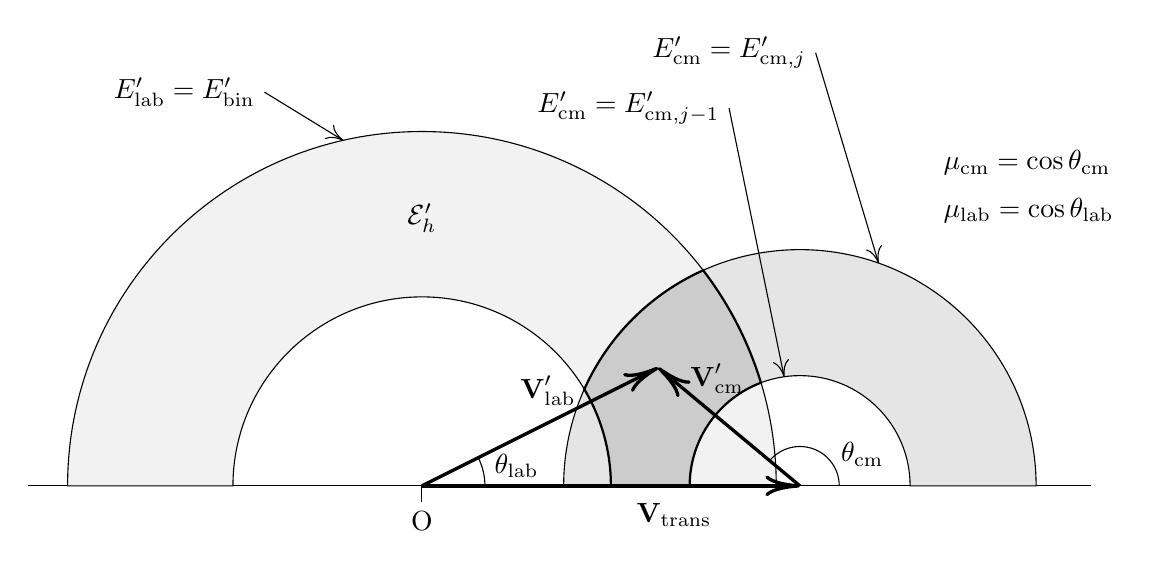
\begin{tikzpicture}
% the axis
\draw [thin] (-5, 0) -- (0, 0);
\draw [thin] (4.8, 0) -- (8.5, 0);
% energy bin
\filldraw[thin, fill = gray!10] (4.5, 0) arc (0:180:4.5) --
  (-2.4, 0) arc (180:0:2.4) -- cycle;
% data region
\filldraw[thin, fill = gray!20] (7.8, 0) arc (0:180:3) --
  (3.4, 0) arc (180:0:1.4) -- cycle;
% quadrature region
\filldraw[thick, fill = gray!40] (2.4, 0) arc (0:30.754: 2.4)
 arc(155.853: 114.16: 3)
  arc(37.463: 16.920: 4.5)
  arc(110.700: 180: 1.4) -- cycle;
% \Vlab'
  \draw[-{>[scale=2.5,
          length=5,
          width=3]}, very thick] (0, 0) -- (3, 1.5);
%  \draw[->, angle 45, very thick] (0, 0) -- (3, 1.5);
% \Vtrans
  \draw[-{>[scale=2.5,
          length=5,
          width=3]}, very thick] (0, 0) -- (4.8, 0);
% \Vcm'
  \draw[-{>[scale=2.5,
          length=5,
          width=3]}, very thick] (4.8, 0) -- (3, 1.5);
% labels
 \node at (0, 3.4) { $\calE_h'$};
 \draw (0, -0.2) -- (0, 0);
 \node [below] at (0, -0.2) {O};
 \draw (0.8, 0) arc ( 0: 26.565: 0.8);
 \node [right] at (0.8, 0.25) {$\theta_{\text{lab}}$};
 \draw (5.3, 0) arc ( 0: 140.194: 0.5);
 \node [right] at (5.2, 0.4) {$\theta_{\text{cm}}$};
 \node [below] at (3.2, -0.1) {$\Vtrans$};
 \node [above] at (3.75, 1.05) {$\Vcm'$};
 \node [above] at (1.6, 0.9) {$\Vlab'$};
 \draw[{<[scale=2, length=3, width=3]}-] (4.6, 1.38560) -- (3.9, 4.8);
 \node[left] at (3.9, 4.8) {$E'_{\text{cm}} = E'_{\text{cm},j-1}$};
 \draw[{<[scale=2, length=3, width=3]}-] (5.8, 2.8284) -- (5, 5.5);
 \node[left] at (5, 5.5) {$E'_{\text{cm}} = E'_{\text{cm},j}$};
 \draw[{<[scale=2, length=3, width=3]}-] (-1, 4.3875) -- (-2, 5);
 \node [left] at (-2, 5) {$\Elab' = \Ebin'$};
 % legend
 \node [right] at (6.5, 4.1) {$\mucm = \cos \theta_{\text{cm}}$};
 \node [right] at (6.5, 3.5)  {$\mu_{\text{lab}} = \cos \theta_{\text{lab}}$};
\end{tikzpicture}
\caption{Integration region over $\Ecm'$ and $\mucm$ for the outgoing energy bin
$\calE_h'$ at a fixed incident energy
for data given at energies $E'_{\text{cm},j-1} \le \Ecm' \le E'_{\text{cm},j}$
in the center-of-mass frame}
\label{Fig:boost-regions}
\end{center} 

\end{figure}

\section{Geometrical considerations}
\label{Sec:boost-geometry}
The first question in the analysis of the integral in Eq.~(\ref{Inum-Legendre-cm})
is the determination of the set~$\calD_{h, \text{cm} }$.  This requires
knowing whether or not the arc for a bin boundary $\Elab' = \Ebin'$ 
intersects an arc $\Ecm' = E'_{\text{cm},j}$ derived from a data point.  For a boost
to the laboratory frame using Newtonian mechanics as in Eq.~(\ref{E_lab}),
this identification is achieved by the function
\begin{equation}
  G_0( \Ebin',  \Ecm', E ) = 2 \Ebin'( \Etrans' + \Ecm' ) -
    ( \Etrans' - \Ecm' )^2 - {\Ebin'}^2.
  \label{def-G0}
\end{equation}
Note that in $G_0$ the dependence on the energy $E$ of the
incident particle typically enters in two ways.  For one thing, 
$\Etrans'$ depends on $E$ as
in Eq.~(\ref{E_trans}).  On the other hand, if the interpolation with
respect to incident energy is unit-base or by cumulative 
points, then the inversion of the unit-base map Eq.~(\ref{range-inv}) 
takes the form
\begin{equation}
  \Ecm' = E'_{\text{cm}, \text{min}} +
     ( E'_{\text{cm}, \text{max}} - E'_{\text{cm}, \text{min}} ) 
    \widehat \Ecm'.
 \label{Kalb-unit-base}
\end{equation}
In linear-linear unit-base interpolation, $\widehat \Ecm'$ is fixed in
the interval $0 \le \widehat \Ecm' \le 1$, while
$E'_{\text{cm}, \text{min}}$
and $E'_{\text{cm}, \text{max}}$ depend on $E$ according to
Eq.~(\ref{EoutRange}) with $q$ given by Eq.~(\ref{def-q}).

The utility of the function $G_0$ in Eq.~(\ref{Kalb-unit-base})
depends on the following result.

\subsection{Assertion}\label{Sec:assertion8}
\textit{In Figure~\ref{Fig:boost-regions} under a Newtonian boost at fixed incident energy $E$, 
an arc $\Elab' = \Ebin'$ representing an edge of an energy bin in
the laboratory frame intersects an arc
$\Ecm' = {\rm const}$ generated by data
in the center-of-mass frame  if and only if}
\begin{equation}
   G_0( \Ebin', \Ecm', E ) \ge 0.
  \label{G0-pos}
\end{equation}

This assertion is proved in Appendix~\ref{Sec:Appendix-B}.

One application of Assertion~\ref{Sec:assertion8} is that of finding the incident energies
$E$ in $\calE_g$ in the integral Eq.~(\ref{Inum-Legendre-cm}) such that
the set $\calD_{h, \text{cm} }$ is non-empty.  This may be done by
locating the zeros of $G_0( \Ebin',  \Ecm', E )$ as a function of $E$
with the edges of the bin $\calE_h'$ as values of $\Ebin'$ and with
$\Ecm'$ as in Eq.~(\ref{Kalb-unit-base}) for 
$$
  \widehat \Ecm' = \widehat E'_{\text{cm}, j-1}
  \quad \text{and} \quad
  \widehat \Ecm' = \widehat E'_{\text{cm}, j},
$$
according to the data.

\section{Input of Legendre coefficients of energy-angle probability
densities in the center-of-mass frame}
The format for input of the coefficients $\pi_\ell( \Ecm' \mid E)$
in Eq.~(\ref{pi-Legendre-cm}) is that of Section~\ref{Sec:ENDF-I4-data}
with some obvious modifications.  For one thing, the data are in
the center-of-mass frame\\
 \Input{Product Frame: CenterOfMass}{}
 
The other difference is that information on particle masses is
required by the boost to the laboratory frame\\
  \Input{Projectile's mass:}{$\myi$} \\
 \Input{Target's mass:}{$\mtarg$} \\
 \Input{Product's mass:}{$\myo$} \\
 \Input{Reaction's Q value:}{$Q$} \\
The values of these quantities must be in the same units as
the energy bin boundaries.

The code computes the mass of the residual from the $Q$ value and
the masses of the other particles.  If the input file also contains the line\\
 \Input{Residual's mass:}{$\mres$}\\
the code compares this value with the mass it computed, printing
a warning message if they are significantly different.

Currently, the boost for this type of data is only implemented using Newtonian mechanics.

\section{Input of isotropic energy probability
densities in the center-of-mass frame}
\label{Sec:isotropic-table-cm}

The format for isotropic energy probability
density data given in the center-of-mass frame is the
same as that for laboratory-frame data in
Section~\ref{Sec:isotropic-table-lab}, except that
the line\\
  \Input{Product Frame: lab}{}\\
is replaced by\\
 \Input{Product Frame: CenterOfMass}{}

\chapter{Joint energy-angle probability density tables}
\label{Sec:joint-table}
It is also possible to give energy-angle probability densities
as tables in \xendl.  These probability tables must be in the 
laboratory coordinate system.
The \ENDL~\cite{Omega} and \ENDF~\cite{ENDFB} forms of these
tables differ slightly, and \gettransfer\ supports both formats.
The \ENDF\ format is described first.

One format for tables
of values of $\pi(\Elab', \mulab \mid E)$ is as arrays
\begin{equation}
  \{ E, \{ \mulab, \{ \Elab', \pi(\Elab', \mulab \mid E) \} \} \}.
 \label{ENDF-E-mu-table}
\end{equation}
The data for the lowest incident energy $E$ are given first,
and data for a given incident energy are ordered by increasing direction cosine $\mulab$.
For fixed $E$ and $\mulab$, the data consist of pairs $\{ \Elab', \pi(\Elab', \mulab \mid E) \}$
for values of the energy $\Elab'$ of the outgoing particle.
The normalization of the data $\pi(\Elab', \mulab \mid E)$ is such that 
for each incident energy $E$
the total probability is
$$
  \int_0^\infty d\Elab' \, \int_{-1}^1 d\mulab \, \pi(\Elab', \mulab \mid E) = 1.
$$

The \ENDL\ energy-angle probability density data tables
are given in the form of the product
\begin{equation}
  \pi(\Elab', \mulab \mid E) =
  \pi_\mu(\mulab \mid E)\pi_E(\Elab' \mid E, \mulab),
   \label{correlated}
\end{equation}
in which $\pi_E(\Elab' \mid E, \mulab)$ is normalized so that
$$
  \int_0^\infty d\Elab' \, \pi_E(\Elab' \mid E, \mulab) = 1
$$
for each of the tabulated values of $E$ and~$\mulab$.

In the \gettransfer\ code energy-angle probability density
tables in the format of Eq.~(\ref{ENDF-E-mu-table}) are converted to
the format of Eq.~(\ref{correlated}) via the formulas
$$
  \pi_\mu(\mulab \mid E) = \int_0^\infty d\Elab' \, \pi(\Elab', \mulab \mid E)
$$
and
$$
  \pi_E(\Elab' \mid E, \mulab) = \frac
    {\pi(\Elab', \mulab \mid E)} {\pi_\mu(\mulab \mid E)}.
$$
The rest of the discussion of energy-angle probability density
tables is therefore in terms of the form of the data in Eq.~(\ref{correlated}).
Tbus, the discussion is in terms of the angular probability density $\pi_\mu(\mulab \mid E)$
and the outgoing energy conditional probability density $\pi_E(\Elab' \mid E, \mulab)$.

With the correlated energy-angle probability density
(\ref{correlated}) the number-preserving integral (\ref{Inum}) is
\begin{multline}
   \Inum_{gh,\ell} =
        \int_{\calE_g} dE \, \sigma ( E ) M(E) w(E) \widetilde \phi_\ell(E) 
       \, \int_{\calE_h' } d\Elab' \, \\
       \, \int_{\mulab} d\mulab \,  P_\ell( \mulab ) \pi_\mu(\mulab \mid E)\pi_E(\Elab' \mid E, \mulab),
  \label{Inum-corr}
\end{multline}
and the energy-preserving integral (\ref{Ien}) becomes
\begin{multline}
  \Ien_{gh,\ell} =
     \int_{\calE_g} dE \, \sigma ( E ) M(E) w(E) \widetilde \phi_\ell(E) 
     \, \int_{\calE_h' } d\Elab' \,  \Elab' \\
     \, \int_{\mulab} d\mulab  \,  P_\ell ( \mulab ) \pi_\mu(\mulab \mid E)\pi_E(\Elab' \mid E, \mulab).
  \label{Ien-corr}
\end{multline}

The method used by \gettransfer\ to evaluate the integrals (\ref{Inum-corr})
and (\ref{Ien-corr}) is to first compute the Legendre coefficients
\begin{equation}
  \pi_\ell(\Elab' \mid E) =
  \int_{-1}^1 d\mulab  \,  P_\ell ( \mulab ) \pi_\mu(\mulab \mid E)\pi_E(\Elab' \mid E, \mulab).
  \label{get-I4}
\end{equation}
The coding for the integration of (\ref{InumI4})
and~(\ref{IenI4}) is then applied to obtain the transfer matrix.

\section{Input of $\pi(\Elab', \mulab \mid E)$ the form of a table, Eq.~(\ref{ENDF-E-mu-table})}
For tables of the energy-angle probability density $\pi(\Elab', \mulab \mid E)$
in the format Eq.~(\ref{ENDF-E-mu-table}), the identification line in
Section~\ref{model-info} is\\
      \Input{Process: ENDF Double differential EMuEpP data}{}\\
These data are always in the laboratory frame,\\
  \Input{Product Frame: lab}{}

The first lines in the data for Section~\ref{model-info} give the number~$K$
of incident energies along with the interpolation rules\\
  \Input{EMuEpPData:}{$n = K$}\\
  \Input{Incident energy interpolation:}{probability interpolation flag}\\
  \Input{Outgoing cosine interpolation:}{probability interpolation flag}\\
  \Input{Outgoing energy interpolation:}{list interpolation flag}\\
The flags for interpolation with respect to incident energy~$E$ and
direction cosine~$\mulab$ are those for probability density tables in
Section~\ref{interp-flags-probability}, and that for outgoing energy~$E'$ is
one for simple lists.

For each incident energy~$E$ there is a data section of the form\\
    \Input{ Ein:}{$E$: \quad \texttt{n = $N$}}\\
indicating that data are given for $N$ values of $\mulab$.  The block of
data corresponding to a value of $\mulab$ is of the form\\
    \Input{ mu:}{$\mulab$: \quad \texttt{n = $J$}}\\
followed by $J$ pairs of values of outgoing energy $\Elab'$ and
probability density~$\pi(\Elab', \mulab \mid E)$ .

An example of such data with energy in MeV is\\
  \Input{EMuEpPData: n = 18}{}\\
  \Input{Incident energy interpolation: lin-lin unitbase}{}\\
  \Input{Outgoing cosine interpolation: lin-lin unibase}{}\\
  \Input{Outgoing energy interpolation: lin-lin }{}\\
  \Input{ Ein: 1.748830e+00:  n = 21}{}\\
  \Input{  mu: -1.000000e+00:  n = 15}{}\\
  \Input{ \indent   1.092990e-03  0.000000e+00}{}\\
  \Input{ \indent   1.093000e-03  7.406740e-01}{}\\
  \Input{ \indent   3.278900e-03  1.166140e+00}{}\\
  \Input{ \indent   7.650800e-03  1.466540e+00}{}\\
  \Input{ \indent   1.202300e-02  1.585880e+00}{}\\
  \Input{ \indent   2.076600e-02  1.610940e+00}{}\\
   \Input{ \indent 2.951000e-02  1.546240e+00}{}\\
\Input{ \indent  5.574100e-02  1.071950e+00}{}\\
\Input{ \indent  7.104300e-02  7.097100e-01}{}\\
\Input{ \indent  8.197300e-02  4.021720e-01}{}\\
 \Input{ \indent 9.071600e-02  1.795810e-01}{}\\
\Input{ \indent  9.508800e-02  9.526480e-02}{}\\
\Input{ \indent  9.946000e-02  2.867760e-02}{}\\
 \Input{ \indent 1.016500e-01  4.692750e-03}{}\\
\Input{ \indent  1.016510e-01  0.000000e+00}{}\\
\Input{ $\cdots$}{}\\
\Input{ Ein: 2.000000e+01:  n = 21}{}\\
 \Input{  mu: -1.000000e+00:  n = 76}{}\\
\Input{ \indent  4.606790e-02  0.000000e+00}{}\\
\Input{ \indent  4.606800e-02  3.837140e-02}{}\\
\Input{ \indent  9.213400e-02  4.393050e-02}{}\\
\Input{ \indent  1.842700e-01  4.977660e-02}{}\\
\Input{ \indent  2.764100e-01  4.806820e-02}{}\\
\Input{ \indent  3.685400e-01  4.385540e-02}{}\\
\Input{ \indent  6.449500e-01  2.695920e-02}{}\\
\Input{ \indent  7.370900e-01  2.255450e-02}{}\\
 \Input{ \indent }{ etc.}

\section{Input of $\pi(\Elab', \mulab \mid E)$ as a product, Eq.~(\ref{correlated})}
For tables of the energy-angle probability density $\pi(\Elab', \mulab \mid E)$
given as the product in Eq.~(\ref{correlated}), the identification line in
Section~\ref{model-info} is\\
      \Input{Process: Double differential EMuEpP data transfer matrix}{}\\
These data are always in the laboratory frame,\\
  \Input{Product Frame: lab}{}

The model-dependent portion of the input file in Section~\ref{model-info}
contains a section for the angular probability density $\pi_\mu(\mulab \mid E)$
and another for the conditional probability density $\pi_E(\Elab' \mid E, \mulab)$.

The section for angular probability density starts with the lines\\
  \Input{Angular data:}{$n = K$}\\
  \Input{Incident energy interpolation:}{probability interpolation flag}\\
  \Input{Outgoing cosine interpolation:}{list interpolation flag}\\
where $K$ is the number of incident energies~$E$.  The flag for
interpolation with respect to incident energy is one of those for
probability density tables in Section~\ref{interp-flags}, and that for 
the direction cosine $\mulab$ is one of those 
for simple lists.  There follows $K$ blocks of data,
one for each incident energy\\
    \Input{ Ein:}{$E$: \quad \texttt{n = $N$}}\\
indicating that data are given for $N$ pairs of values of $\mulab$
and $\pi_\mu(\mulab \mid E)$.

The section for conditional probability density of outgoing energy
$\pi_E(\Elab' \mid E, \mulab)$ gives the number~$K$
of incident energies along with the interpolation rules\\
  \Input{EMuEpPData:}{$n = K$}\\
  \Input{Incident energy interpolation:}{probability interpolation flag}\\
  \Input{Outgoing cosine interpolation:}{probability interpolation flag}\\
  \Input{Outgoing energy interpolation:}{list interpolation flag}\\
The flags for interpolation with respect to incident energy~$E$ and
direction cosine~$\mulab$ are those for probability density tables in
Section~\ref{interp-flags-probability}, and that for outgoing energy~$E$ is one of those
for simple lists.

For each incident energy~$E$ there is a data section of the form\\
    \Input{ Ein:}{$E$: \quad \texttt{n = $N$}}\\
indicating that data are given for $N$ values of $\mulab$.  The block of
data corresponding to a value of $\mulab$ is of the form\\
    \Input{ mu:}{$\mulab$: \quad \texttt{n = $J$}}\\
followed by $J$ pairs of values of outgoing energy $E$ and
probability density~$\pi_E(\Elab' \mid E, \mulab)$.

An example of this type of data with energy in MeV is given by\\
  \Input{Angular data: n = 13}{}\\
  \Input{Incident energy interpolation: lin-lin unitbase}{}\\
  \Input{Outgoing cosine interpolation: lin-lin}{}\\
  \Input{ Ein:   7.78148000e+00:  n = 5}{}\\
  \Input{ \indent   9.99788143e-01   5.88016882e+01}{}\\
  \Input{ \indent   9.99841107e-01   1.03998708e+03}{}\\
  \Input{ \indent   9.99894071e-01   1.70086214e+03}{}\\
  \Input{ \indent   9.99947036e-01   2.60922780e+03}{}\\
  \Input{ \indent   1.00000000e+00   2.70023193e+04}{}\\
  \Input{ $\cdots$}{}\\
   \Input{ Ein: 2.00000000e+02: n = 5}{}\\
 \Input{ \indent -1.00000000e+00  3.26136085e-01}{}\\
 \Input{ \indent -5.00000000e-01  3.82892835e-01}{}\\
  \Input{ \indent 0.00000000e+00  4.64096868e-01}{}\\
  \Input{ \indent 5.00000000e-01  5.89499334e-01}{}\\
  \Input{ \indent 1.00000000e+00  8.00885838e-01}{}\\
   \Input{EMuEpPData: n = 13}{}\\
  \Input{Incident energy interpolation: lin-lin unitbase}{}\\
  \Input{Outgoing cosine interpolation: lin-lin unitbase}{}\\
  \Input{Outgoing energy interpolation: lin-lin}{}\\
  \Input{ Ein:   7.78148000e+00:  n = 5}{}\\
  \Input{ mu:   9.99788143e-01:  n = 4}{}\\
  \Input{ \indent   2.35390141e-03  1.62759930e+05}{}\\
  \Input{ \indent   2.35697064e-03  1.62877493e+05}{}\\
  \Input{ \indent   2.35697074e-03  1.62877496e+05}{}\\
  \Input{ \indent   2.36004196e-03  1.62892892e+05}{}\\
  \Input{ mu:   9.99841107e-01:  n = 16}{}\\
  \Input{ \indent   2.30884914e-03  9.56657064e+03}{}\\
   \Input{ \indent  2.32094195e-03  9.99310479e+03}{}\\
   \Input{ \indent}{ etc.}\\
 \Input{ Ein:  2.00000000e+02: n = 5}{}\\
\Input{  mu: -1.00000000e+00: n = 501}{}\\
  \Input{ \indent 1.00000000e-18  5.38736174e-10}{}\\
  \Input{ \indent 1.00563208e-17  1.70842412e-09}{}\\
  \Input{ \indent 1.91126417e-17  2.35524717e-09}{}\\
  \Input{ \indent 2.81689625e-17  2.85931206e-09}{}\\
  \Input{ \indent 3.72252834e-17  3.28696542e-09}{}\\
  \Input{ $\cdots$}{}\\
  \Input{ mu: 1.00000000e+00: n = 993}{}\\
  \Input{ \indent 1.00000000e-18  2.19383712e-10}{}\\
  \Input{ \indent 7.55831305e-18  6.03138181e-10}{}\\
  \Input{ \indent }{ $\cdots$}\\
  \Input{ \indent 1.32751551e+01  1.88436981e-03}{}\\
  \Input{ \indent 1.38015128e+01  1.90038969e-03}{}
 
 
\chapter{Formulas for double-differential energy-angle data}
\label{Sec:double-diff-formula}
This section explains the coding used to treat two representations
by formula for double-differential energy-angle data in the \xendl\ library,
the Kalbach-Mann formula and the phase-space model.  The
Kalbach-Mann model is described first, because it is used so often in \xendl.

\section{The Kalbach-Mann model for double-differential data}
In the Kalbach-Mann representation \cite{Kalbach} the
double differential probability density is of the form
\begin{equation}
  \pi(\Ecm', \mucm \mid E) =
  \pi_E( \Ecm' \mid E) \pi_\mu( \mucm \mid \Ecm', E ),
  \label{Kalbach-prob}
\end{equation}
where $E$ is the energy of the incident particle in laboratory
coordinates and $\Ecm'$ and $\mucm$ are the energy and cosine of
the outgoing particle in center-of-mass coordinates.
The values of the probability density $\pi_E( \Ecm' \mid E)$ for outgoing 
energy $\Ecm'$
are given as a table with normalization
$$
  \int_0^\infty d\Ecm' \, \pi_E( \Ecm' \mid E) = 1.
$$
In Eq.~(\ref{Kalbach-prob}) the function
$\pi_\mu( \mucm \mid \Ecm', E )$ is an exponential in
$\mucm$ depending on parameters~$a$ and~$r$~\cite{Kalbach},
\begin{equation}
  \pi_\mu( \mucm \mid \Ecm', E ) =
    \frac{1}{C}
    [ \cosh(a\mucm) + r \sinh(a\mucm)].
  \label{Kalbach-eta}
\end{equation}
The value of $r$ in Eq.~(\ref{Kalbach-eta}) depends on the incident and outgoing energies 
$E$ and $\Ecm'$ and is given in a data table.  The formula Eq.~(\ref{Kalbach-eta})
represents a pre-equilibrium model, with $r=0$ representing complete
equilibrium and $r = 1$ no equilibrium at all.  It is therefore always true
that
$$
  0 \le r \le 1.
$$

The value of $C$ in Eq.~(\ref{Kalbach-eta}) is chosen to ensure the normalization
$$
  \int_{-1}^1 d\mucm \, \pi_\mu( \mucm \mid \Ecm', E ) = 1.
$$
That is, take
$$
  C = \frac{ 2 \sinh{a}}{a}.
$$

\subsection{The Kalbach-Mann $a$ parameter}
The values of the parameter~$a$ in Eq.~(\ref{Kalbach-eta}) may be given
as a table depending on the incident
energy $E$ and on $\Ecm'$, the center-of-mass kinetic energy of
the outgoing particle.  It is more common, however, to use the formula
for $a$ as a function of $E$ as found in the references \cite{Kalbach} and~\cite{ENDFB}.
The details are repeated here for the sake of completeness.

{% begin special notation
\newcommand{\Ealab}{E_{a,\text{lab}}}
\newcommand{\Eacm}{E_{a,\text{cm}}}
\newcommand{\EAcm}{E_{A,\text{cm}}}
\newcommand{\EaAcm}{E_{aA,\text{cm}}}
\newcommand{\Ebcm}{E_{b,\text{cm}}}
\newcommand{\EBcm}{E_{B,\text{cm}}}
\newcommand{\EbBcm}{E_{bB,\text{cm}}}
Some special notation is used in this subsection.  The reaction is of the form
\begin{equation}
  A + a \to C \to B + b,
 \label{Kalbach-reaction}
\end{equation}
where
\begin{align*}
  A:\quad &\text{the target with mass $\mtarg$, assumed to be at rest in the laboratory frame,} \\
  a:\quad &\text{the incident particle with mass $\myi$,} \\
  C:\quad &\text{the compound nucleus,} \\
  B:\quad &\text{the residual nucleus with mass $\mres$,} \\
  b:\quad &\text{the emitted particle with mass $\myo$.}
\end{align*}


Several energies are needed, all measured in MeV,
\begin{align*}
  \Ealab:\quad &\text{energy of the incident particle in the laboratory frame,} \\
  \Eacm:\quad &\text{energy of the incident particle in the center-of-mass frame,} \\
  \EAcm:\quad &\text{energy of the target in the center-of-mass frame,} \\
  \EaAcm:\quad &\Eacm + \EAcm = \mtarg \Ealab/( \mtarg + \myi), \\
  \Ebcm:\quad &\text{energy of the outgoing particle in the center-of-mass frame,} \\
  \EbBcm:\quad & (\mres + \myo) \Ebcm / \myo.
\end{align*}
Note that the quantity $\EbBcm$ is the total kinetic energy of $B$ and $b$ if
the breakup of $C$ is a discrete 2-body reaction with the excitation level
of $B$ unspecified.

For a reaction with several outgoing particles, $b$ in Eq.~(\ref{Kalbach-reaction})
is the particle corresponding to the current data, and $B$ is the residual
following the emission of $b$ from the compound nucleus~$C$.
Thus, for the
$$
   {}^{78}\text{Kr} (n, np) {}^{77}\text{Br}
$$
reaction, one uses
$$
   B =  {}^{78}\text{Kr}
$$
in the computation of $a(E, \Ebcm)$ with Kalbach-Mann data for the
outgoing neutron, while
$$
   B =  {}^{78}\text{Br}
$$
with outgoing proton data.  Analogously, use
$$
     B =  {}^{78}\text{Kr}
$$
in the computation of $a(E, \Ebcm)$ with Kalbach-Mann neutron data for the
$$
   {}^{78}\text{Kr} (n, 2n) {}^{77}\text{Kr}
$$
reaction.

For massive incident particles, the value of $a(E, \Ebcm)$ is given 
by the expression
\begin{equation}
  a(E, \Ebcm) = C_1 X_1 + C_2 X_1^3 + C_3 M_a m_b X_3^4
 \label{Kalbach-a}
\end{equation}
with terms explained below.

The coefficients in Eq.~(\ref{Kalbach-a}) are
$$
  C_1 = 0.04\,\text{MeV}^{-1}, \quad
  C_2 = 1.8 \times 10^{-6}\,\text{MeV}^{-3}, \quad
  C_3 = 6.7 \times 10^{-7} \,\text{MeV}^{-4}.
$$

The values of $X_1$ and $X_3$ in Eq.~(\ref{Kalbach-a}) depend on
the energies $S_a$ and $S_b$ of the capture and breakup  reactions
in Eq.~(\ref{Kalbach-reaction}).  For the target define
\begin{align*}
  Z_A: \quad & \text{number of protons in the target nucleus,} \\
  N_A: \quad & \text{number of neutrons in the target nucleus,} \\
  A_A: \quad & Z_A + N_A.
\end{align*}
Corresponding $Z_C$, $N_C$, and $A_C$ are defined  
for the compound nucleus~$C$ and
$Z_B$, $N_B$, and $A_B$ for the residual nucleus~$B$.
For the capture reaction,
$S_a$ is taken as
\begin{multline}
  S_a = 15.68(A_C - A_A) -
    28.07\left(
      \frac{(N_C - Z_C)^2}{A_C} - \frac{(N_A - Z_A)^2}{A_A }
    \right) - {} \\
    18.56( A_C^{2/3} - A_A^{2/3}) +
      33.22\left(
        \frac{(N_C - Z_C)^2}{A_C^{4/3}} - \frac{(N_A - Z_A)^2}{A_A^{4/3} }
    \right) - {} \\
    0.717\left(
      \frac{Z_C^2}{A_C^{1/3}} - \frac{Z_A^2}{A_A^{1/3}}
    \right) + 1.211\left(
      \frac{Z_C^2}{A_C} - \frac{Z_A^2}{A_A}
    \right) - I_a.
 \label{def-Sa}
\end{multline}
Here, $I_a$ is the breakup energy for the incident particle
as given in Table~10.1.  The energy $S_b$ corresponding to the second
reaction in Eq.~(\ref{Kalbach-reaction}) is obtained from Eq.~(\ref{def-Sa})
with $Z_A$, $N_A$, $A_A$, and $I_a$ replaced, respectively by
$Z_B$, $N_B$, $A_B$, and $I_b$.

\begin{table}
\caption{Breakup energies for incident and outgoing particles in MeV}
$$
 \vbox{ \offinterlineskip \tabskip = 0.0cm
  \halign{
   \mystrut#\hfil  \tabskip = 0.5cm &
   \hfil#\hfil&
   \hfil#\hfil&  \tabskip = 0cm
   \hfil\vrule#\cr
   \noalign{\hrule}
   height 12pt depth 6pt& particle&  $I_a$ or $I_b$& \cr
   \noalign{\hrule}
   height 12pt& $n$& 0& \cr
   &$p$& 0& \cr
   &$d$& 2.22& \cr
   &$t$& 8.48& \cr
   &${}^3\text{He}$& 7.72& \cr
   depth 6pt &$\alpha$& 28.3& \cr
   \noalign{\hrule}
  }
 }
$$
\end{table}

The quantities $X_1$ and $X_3$ in Eq.~(\ref{Kalbach-a}) are
obtained by setting
\begin{alignat*}{2}
   \textbf{E}_a &= \EaAcm + S_a, \qquad
    & \textbf{E}_b &= \EbBcm + S_b, \\
   E_{t1} &= 130 \text{ MeV}, \qquad
    & E_{t3} &= 41 \text{ MeV}, \\
   R_1 &= \min( \textbf{E}_a, E_{t1}), \qquad
    & R_3 &= \min( \textbf{E}_a, E_{t3}), \\
   X_1 &= R_1 \textbf{E}_b / \textbf{E}_a, \qquad
    & X_3 &= R_3 \textbf{E}_b / \textbf{E}_a.
\end{alignat*}

Finally the values $M_a$ for the incident particle and $m_b$ for the
outgoing particle in the last term of Eq.~(\ref{Kalbach-a}) are
given in Table~10.2.  Note that $M_a$ is not defined for incident
tritons or for incident helium-3 nuclei, so that the Kalbach-Mann
model is not applicable when the incident energy of such 
particles is so large that $\textbf{E}_a > E_{t3}$.

\begin{table}
\caption{Values of $M_a$ and $m_b$ in Eq.~(\ref{Kalbach-a})}
$$
 \vbox{ \offinterlineskip \tabskip = 0.0cm
  \halign{
   \mystrut#\hfil  \tabskip = 0.5cm &
   \hfil#\hfil&
   \hfil#\hfil&
   \hfil#\hfil&  \tabskip = 0cm
   \hfil\vrule#\cr
   \noalign{\hrule}
   height 12pt depth 6pt& particle&  $M_a$& $m_b$& \cr
   \noalign{\hrule}
   height 12pt& $n$& 1& 1/2 &\cr
   &$p$& 1& 1&\cr
   &$d$& 1& 1& \cr
   &$t$& ---& 1& \cr
   &${}^3\text{He}$& ---& 1&\cr
   depth 6pt &$\alpha$& 0& 2& \cr
   \noalign{\hrule}
  }
 }
$$
\end{table}

\subsection{Photo-nuclear reactions}
When Kalbach-Mann data are given for photo-nuclear reactions, 
the parameter $a(E, \Ebcm)$ in Eq.~(\ref{Kalbach-a}) and the
angular probability density $\pi_\mu( \mucm \mid \Ecm', E )$
in Eq.~(\ref{Kalbach-eta}) are modified as in the paper~\cite{photo-nuc}.

One begins by computing $a_n(E, \Ebcm)$ in Eq.~(\ref{Kalbach-a}) using a neutron as
incident particle.  Then, for the incident photon one takes
\begin{equation}
  a(E, \Ebcm) = a_n(E, \Ebcm)
    \sqrt{ \frac{E}{2 m_n} } \,
    \min\left(
      4, \max\left(
        1, \frac{9.3}{\sqrt{\Ebcm}}
      \right)
    \right).
 \label{Kalbach-photo}
\end{equation}
Here, $m_n$ is the mass of the neutron in MeV.

For incident photons the angular probability density takes the form
$$
  \pi_\mu( \mucm \mid \Ecm', E ) =
  \frac{1}{2} \left[
    (1 - r) + \left(
      \frac{ar}{\sinh(a)}
    \right) \expon{a \mucm}
  \right].
$$


\subsection{Interpolation of Kalbach-Mann data}\label{Sec:Kalbach-Mann-interp}

In the \xendl\ library, the Kalbach-Mann data are given
as a table of the probability density $\pi_E( \Ecm' \mid E)$ of outgoing
energy~$\Ecm'$ for an incident particle with energy~$E$,
along with a table of values of the parameter~$r$ in Eq.~(\ref{Kalbach-eta})
as a function of $E$ and~$\Ecm'$.  It is also permitted to include a
table of values $a(E,  \Ebcm)$ to be used in place of the expression
in Eq.~(\ref{Kalbach-a}).
}% end special notation

Because $\pi_E( \Ecm' \mid E)$ is a probability
density, it is to be interpolated with respect to $E$ by one of the methods
of Section~\ref{Sec:2d-interp}.  
The interpolated values of $r$, however, must 
maintain the physical constraints that $0 \le r \le 1$,
so the Kalbach-Mann $r$ parameter is interpolated by the unscaled methods of
Section~\ref{Sec:Kalbach-r-interp}.  If the values of $a$ are also
given as a table, they are also interpolated as in Section~\ref{Sec:Kalbach-r-interp}.

For unit-base interpolation the method is as follows.
The energy probability density
$\pi_E( \Ecm' \mid E)$ is first mapped to unit base as defined in equations
Eqs.~(\ref{unit-base-map}) and~(\ref{unitbaseMap}), so that
\begin{equation}
  \widehat \pi_E( \widehat \Ecm' \mid E) =
    ( E'_{\text{cm}, \text{max}} - E'_{\text{cm}, \text{min}} ) 
     \pi_E( \Ecm' \mid E)
 \label{Kalb-pi-unit-base}
\end{equation}
for $0 \le \widehat \Ecm' \le 1$.
The scale factor in Eq.~(\ref{Kalb-pi-unit-base}) is chosen so as to 
normalize the function $\widehat \pi_E( \widehat \Ecm' \mid E) $,
$$
  \int_0^1 d\widehat \Ecm' \, \pi_E( \widehat \Ecm' \mid E) = 1.
$$
The values of $\widehat \pi_E( \widehat \Ecm' \mid E)$ are
interpolated linearly with respect to $E$.

For the values of the parameter $r$, the energy
of the outgoing particle to is mapped $0 \le \widehat \Ecm' \le 1$
using Eq.~(\ref{Kalb-unit-base}) in the form of
$$
  \widehat \Ecm' = \frac{
  \Ecm' - E'_{\text{cm}, \text{min}} }
     { E'_{\text{cm}, \text{max}} - E'_{\text{cm}, \text{min}} }.
$$
Because of the
restriction that $0 \le r \le 1$, the parameter $r$ is mapped according to
\begin{equation}
  \widetilde r( \widehat \Ecm', E ) = r( \Ecm', E ).
  \label{map-Kalb-r}
\end{equation}

With these transformations, the number-preserving integral Eq.~(\ref{Inum}) 
takes the form
\begin{multline}
   \Inum_{gh,\ell} =
         \int_{\calE_g} dE \, \sigma ( E ) M(E) w(E) \widetilde \phi_\ell(E) 
       \, \int_{\widehat \Ecm' } d\widehat \Ecm' \,
           \widehat \pi_E( \widehat \Ecm' \mid E) \\
        \int_{\mucm} d\mucm \,  P_\ell( \mulab ) \pi_\mu( \mucm \mid \Ecm', E ),
  \label{Inum-Kalb-corr}
\end{multline}
and the energy-preserving integral Eq.~(\ref{Ien}) becomes
\begin{multline}
  \Ien_{gh,\ell} =
        \int_{\calE_g} dE \, \sigma ( E ) M(E) w(E) \widetilde \phi_\ell(E) 
       \, \int_{\widehat \Ecm' } d\widehat \Ecm' \,
           \widehat \pi_E( \widehat \Ecm' \mid E) \\
        \int_{\mucm} d\mucm \,  P_\ell( \mulab ) \pi_\mu( \mucm \mid \Ecm', E ) \Elab' .
  \label{Ien-Kalb-corr}
\end{multline}
The subscripts on $\mu$ serve to emphasize the facts
that the argument $\mulab$ of the Legendre polynomial
$P_\ell( \mulab )$ in Eqs.~(\ref{Inum-Kalb-corr}) and (\ref{Ien-Kalb-corr}) is
the direction cosine of the outgoing particle in laboratory coordinates,
while the integration variable $\mucm$ is the direction cosine in
center-of-mass coordinates.
Specifically, $\Elab' $ depends on $E$ and $\mucm$ according to equation Eq.~(\ref{E_lab}),
and $\mulab$ is given by Eq.~(\ref{get_mu}).

Because the energy probability density $\pi_E( \Ecm' \mid E)$ data are given
in the center-of-mass frame, the identification of the region of integration
over $\widehat \Ecm'$ and~$\mucm$ in Eqs.~(\ref{Inum-Kalb-corr})
and~(\ref{Ien-Kalb-corr}) involves the geometric considerations
presented for tabular center-of-mass data in Section~\ref{Sec:boost-geometry}.
For a given incident energy $E$ in bin $\calE_g$,
the regions of integration over
$\widehat \Ecm'$ and $\mucm$ in Eqs.~(\ref{Inum-Kalb-corr}) 
and~(\ref{Ien-Kalb-corr}) depend on how the domains for data interpolation
$ \widehat E'_{\text{cm},j-1} \le \widehat \Ecm' \le \widehat E'_{\text{cm},j}$
 intersect
the  $\calE_h'$ outgoing laboratory energy bin.   
The situation for a fixed incident
energy~$E$ is illustrated in Figure~\ref{Fig:boost-regions}.  
The half annulus
$$
  E'_{\text{cm}, j-1} \le \Ecm' \le  E'_{\text{cm}, j}
$$
is derived from the Kalbach-Mann data.  The region of integration 
over $\mucm$ and $\Ecm'$ for fixed incident energy $E$ is the intersection of
these two half annuli, and it is shaded dark gray in Figure~\ref{Fig:boost-regions}.

\subsection{The input file for the Kalbach-Mann model}
The data identifier in Section~\ref{data-model} for the
Kalbach-Mann model is\\
  \Input{Process: Kalbach spectrum}{}\\
and the data are always in the center-of-mass frame\\
  \Input{Product Frame: CenterOfMass}{}\\
Currently, only a Newtonian boost to the laboratory frame is
implemented.

The masses of the particles $a$, $A$, $C$, $b$, and~$B$ in
the reaction Eq.~(\ref{Kalbach-reaction}) are input in Section~\ref{model-info}
of the input file\\
  \Input{Projectile's mass:}{$\myi$} \\
 \Input{Target's mass:}{$\mtarg$} \\
 \Input{Compound's mass:}{$m_C$} \\
 \Input{Product's mass:}{$\myo$} \\
 \Input{Residual's mass:}{$\mres$}\\
The units used for these masses are arbitrary, but they must be the
same for all particles.

The number of protons $Z_A$ and the atomic number $A_A$ of the
target are needed for the computation of $S_a$ in Eq.~(\ref{def-Sa}).
This information is entered into the input file as
$$
  \textsf{ZA}_A = 1000Z_A + A_A,
$$
from which $A_A$, $Z_A$, and the number of neutrons $N_A = A_A - Z_A$
are easily computed.  Corresponding numbers $\textsf{ZA}_a$ for the projectile and
$\textsf{ZA}_b$ for the emitted particle are also given.  The numbers $\textsf{ZA}_C$ for
the compound nucleus and $\textsf{ZA}_B$ for the residual may be calculated
using
\begin{align*}
  \textsf{ZA}_C &= \textsf{ZA}_A + \textsf{ZA}_a,\\
  \textsf{ZA}_B &= \textsf{ZA}_C - \textsf{ZA}_b.
\end{align*}
This section of the input file is therefore\\
  \Input{Projectile's ZA:}{$\textsf{ZA}_a$} \\
 \Input{Target's ZA:}{$\textsf{ZA}_A$} \\
 \Input{Product's ZA:}{$\textsf{ZA}_b$}
 
 The remainder of the input file consists of tables of $\pi_E( \Ecm' \mid E)$
 and the parameter~$r$ in Eq.~(\ref{Kalbach-eta}) as functions of $E$ and~$\Ecm'$.
 There may also be a table of values of $a$ to be used in place of the expression
 Eq.~(\ref{Kalbach-a}).  
 
 The format for the probability density
 $\pi_E( \Ecm' \mid E)$ is\\
   \Input{Kalbach probabilities:}{$n = K$}\\
  \Input{Incident energy interpolation:}{probability interpolation flag}\\
  \Input{Outgoing energy interpolation:}{list interpolation flag}\\
followed by $K$ blocks of the form\\
 \Input{Ein: $E$:}{$n = J$}\\
with $J$ pairs of values of $\Ecm'$ and~$\pi_E( \Ecm' \mid E)$.
The flag for interpolation with respect to incident energy $E$ is
one of those for probability densities in Section~\ref{interp-flags-probability}, 
while that for the outgoing energy
is one for simple lists.

The table for the $r$ parameter is of the form\\
   \Input{Kalbach r parameter:}{$n = K$}\\
  \Input{Incident energy interpolation:}{unscaled interpolation flag}\\
  \Input{Outgoing energy interpolation:}{list interpolation flag}\\
followed by $K$ blocks of the form\\
 \Input{Ein: $E$:}{$n = J$}\\
with $J$ pairs of values of $\Ecm'$ and~$r( \Ecm',  E)$.
The flag for interpolation with respect to incident energy $E$ is
one of those for unscaled Kalbach-Mann data in Section~\ref{interp-flags-Kalbach-r}, 
while that for the outgoing energy
is one for simple lists.

The format for the Kalbach-Mann $a$ parameter is the same as that for $r$,
with ``r'' replaced by ``a''.  \textit{The tables for $\pi_E( \Ecm' \mid E)$, $r$,
and~$a$ must be given at the same incident energies, and at each
incident energy~$E$, the ranges of outgoing energies~$E'$ must also agree.}

An example of the content of Section~\ref{model-info} of the input
file for Kalbach-Mann data is as follows.  All energies are in MeV.\\
 \Input{Product Frame: centerOfMass}{}\\
 \Input{\# masses}{}\\
  \Input{Projectile's mass: 1.008665}{}\\
 \Input{Target's mass: 56.935394}{}\\
 \Input{Compound's mass: 57.933276}{}\\
 \Input{Product's mass: 1.008665}{}\\
 \Input{Residual's mass: 56.935394}{}\\
 \Input{\# ZA numbers}{}\\
  \Input{Projectile's ZA: 1}{}\\
 \Input{Target's ZA: 26057}{}\\
 \Input{Product's ZA: 1}{}\\
 \Input{\# Kalbach-Mann probability data}{}\\
 \Input{Kalbach probabilities:  n = 12}{}\\
 \Input{Incident energy interpolation: lin-lin unitbase}{}\\
 \Input{Outgoing energy interpolation: flat}{}\\
 \Input{ Ein: 7.781480e+00:   n = 2}{}\\
 \Input{ \indent 0.000000e+00   1.000000e+06}{}\\
 \Input{ \indent 1.000000e-06   0.000000e+00}{}\\
 \Input{ Ein: 7.800000e+00:   n = 7}{}\\
 \Input{ \indent 0.000000e+00   7.375605e+00}{}\\
 \Input{ \indent 1.473426e-03   1.472617e+01}{}\\
 \Input{ \indent 3.437994e-03   3.676034e+01}{}\\
 \Input{ \indent 7.367130e-03   5.717426e+01}{}\\
   \Input{ \indent 1.473426e-02  8.186549e+00}{}\\
  \Input{ \indent 3.437994e-02  5.948511e+00}{}\\
  \Input{ \indent 7.367130e-02  1.000000e-30}{}\\
 \Input{ $\cdots$}{}\\
 \Input{ Ein: 2.000000e+01:  n = 53}{}\\
  \Input{ \indent 0.000000e+00  2.063824e-03}{}\\
  \Input{ \indent 1.473426e-03  3.887721e-03}{}\\
  \Input{ \indent 3.437994e-03  9.245874e-03}{}\\
  \Input{ \indent 7.367130e-03  1.805939e-02}{}\\
  \Input{ \indent 1.473426e-02  3.554576e-02}{}\\
  \Input{ \indent 3.437994e-02  8.408804e-02}{}\\
  \Input{ \indent 7.367130e-02  1.261293e-01}{}\\
  \Input{ \indent }{ $\cdots$}\\
  \Input{ \indent 1.154184e+01  1.604784e-03}{}\\
  \Input{ \indent 1.203298e+01  1.000000e-30}{}\\
 \Input{\# Kalbach-Mann r data}{}\\
  \Input{Kalbach r parameter:  n = 12}{}\\
 \Input{Incident energy interpolation: lin-lin unscaledunitbase}{}\\
 \Input{Outgoing energy interpolation: flat}{}\\
 \Input{ Ein: 7.781480e+00:   n = 2}{}\\
 \Input{ \indent 0.000000e+00   0.000000e+00}{}\\
 \Input{ \indent 1.000000e-06  0.000000e+00}{}\\
 \Input{ Ein: 7.800000e+00:   n = 7}{}\\
 \Input{ \indent 0.000000e+00   4.272290e-02}{}\\
 \Input{ \indent 1.473426e-03   2.992310e-02}{}\\
 \Input{ \indent 3.437994e-03   1.833870e-02}{}\\
 \Input{ \indent 7.367130e-03   1.427320e-02}{}\\
   \Input{ \indent 1.473426e-02  1.829320e-02}{}\\
  \Input{ \indent 3.437994e-02  1.611740e-02}{}\\
  \Input{ \indent 7.367130e-02  1.590910e-02}{}\\
 \Input{ $\cdots$}{}\\
 \Input{ Ein: 2.000000e+01:  n = 53}{}\\
  \Input{ \indent 0.000000e+00  7.037570e-02}{}\\
  \Input{ \indent 1.473426e-03  4.957320e-02}{}\\
  \Input{ \indent 3.437994e-03  3.056740e-02}{}\\
  \Input{ \indent 7.367130e-03  2.555550e-02}{}\\
  \Input{ \indent 1.473426e-02  1.908500e-02}{}\\
 \Input{ \indent  $\cdots$}{}\\
 \Input{ \indent 1.154184e+01  9.548000e-01}{}\\
  \Input{ \indent 1.203298e+01  9.656400e-01}{}

\section{The $n$-body phase space model}
The $n$-body phase space model gives the probability density for
the energy of an outgoing particle in center-of-mass coordinates.
The formula is derived from the volume in phase space occupied
by the particles, subject to the constraints of conservation
of energy and momentum.  The model uses Newtonian mechanics.

In the \ENDF\ manual~\cite{ENDFB}
there are two scenarios for this model: (1) inelastic collision
followed by break-up of the excited residual, and (2) break-up
induced by the collision.  In the first case, the $n$-body phase space
model treats only the particles emitted in the break-up of the excited
residual, not the one from the initial collision.  The total kinetic energy $\Estar$
of the outgoing particles treated by the model therefore depends on
the scenario.

In the case of break-up following an
inelastic collision, the analysis is in the frame in which the residual from
the inelastic collision is stationary.  The total kinetic energy of the 
outgoing particles involved is then
$$
  \Estar = Q_{\textrm{res}},
$$
where $Q_{\textrm{res}}$ is
the energy of the break-up of the excited residual.  In this case, the reference
frame for the model is that in which the residual nucleus is stationary
after the initial inelastic collision.  The \gettransfer\ 
code currently does not implement this scenario, because this is
a 2-step reaction.

For the break-up of a compound nucleus following the collision of a projectile
with a stationary target in the laboratory frame, the total kinetic energy $\Estar$
of the outgoing particles in the center-of-mass frame is the sum of two
components, the $Q$ of the reaction plus the energy of the initial collision in the
center-of-mass frame.  For an incident
particle of mass $m_i$ and energy $E$ in the laboratory frame hitting a
stationary target of mass $\mtarg$, this collision energy in the center-of-mass frame is
$$
  \frac{\mtarg E}{\myi + \mtarg}.
$$
Consequently, in this scenario the total center-of-mass kinetic energy for all
outgoing particles is
\begin{equation}
  \Estar = Q + \frac{\mtarg E}{\myi + \mtarg}.
  \label{def-Estar}
\end{equation}

The details of the $n$-body phase space model are as follows.
Consider a particular outgoing particle, and suppose that its mass is~$\myo$.
Then conservation of energy and
momentum implies that the maximum kinetic energy of this particle
in the center-of-mass frame is given by
\begin{equation}
  \Emax = \frac{(M_t - \myo) \Estar}{M_t},
  \label{def-Emax}
\end{equation}
where $M_t$ is the total mass of the outgoing particles covered by
the $n$-body phase space model.

Suppose that $n$ is the number of particles resulting from the break-up
reaction.  For an outgoing particle with mass $\myo$,
let $\Emax$ be as in Eq.~(\ref{def-Emax}).
Then in the $n$-body phase space model, the energy probability density 
that this outgoing particle will have energy $\Ecm'$ with $0 \le \Ecm' \le \Emax$
is given by
\begin{equation}
  \picm(\Ecm' \mid E ) = C_n 
     \sqrt{\Ecm'}\,
     (\Emax - \Ecm')^{(3n - 8)/2}.
  \label{probability}
\end{equation}
Note that this probability density is isotropic in the center-of-mass frame.
Furthermore, the relation Eq.~(\ref{probability}) was derived using Newtonian
mechanics.

The normalization constant $C_n$ in Eq.~(\ref{probability}) is best
represented in terms of the beta function
\begin{equation}
  B(\alpha, \beta) =
   \int_0^1 dt \, t^{\alpha - 1} (1 - t)^{\beta - 1} =
   \frac{\Gamma(\alpha) \Gamma(\beta)}{\Gamma( \alpha + \beta)}.
  \label{beta-func}
\end{equation}
With this notation, it is seen that
\begin{equation}
  \frac{1}{C_n} = B\left(\frac{3}{2}, \frac{3n - 6}{2} \right)
    {\Emax}^{(3n - 5)/2}.
  \label{norm}
\end{equation}

\subsection{Geometry of the $n$-body phase space model}
The construction of Figure~\ref{Fig:boost-regions}
made use of the fact that the tabular data required the
consideration of ranges of energy $\Ecm'$ of the outgoing particle
between the tabulated values,
\begin{equation}
  E'_{\text{cm},j-1} \le \Ecm' \le E'_{\text{cm},j}.
  \label{KalbachEcm}
\end{equation}
Here, the limiting values $E'_{\text{cm},j-1}$ and $E'_{\text{cm},j}$
depend on the energy $E$ of the incident particle according to the
principles of unit-base interpolation in Eq.~(\ref{Kalb-unit-base}).

For the $n$-body phase space model, however, the range of
center-of-mass energies of the outgoing particle is
\begin{equation}
  0 \le \Ecm' \le \Emax,
  \label{nBodyEcm}
\end{equation}
where $\Emax$ is as in Eq.~(\ref{def-Emax}).  
That is, for the $n$-body phase space
the annular ring Eq.~(\ref{KalbachEcm}) in Figure~8.1 is replaced by the
interior of the semicircle Eq.~(\ref{nBodyEcm}).

\subsection{Input file for the $n$-body phase space model}
The data identifier in Section~\ref{data-model} for the
$n$-body phase space model is\\
  \Input{Process: phase space spectrum}{}\\
and the data are always in the center-of-mass frame\\
  \Input{Product Frame: CenterOfMass}{}\\
Currently, only a Newtonian boost to the laboratory frame is
implemented.

In the model-dependent Section~\ref{model-info} of the input file,
the computation of $\Estar$ in Eq.~(\ref{def-Estar}) requires the
reaction's $Q$ value, as well as the masses $\myi$ of the projectile
and $\mtarg$ of the target.  The units used for the masses are arbitrary,
but the same units must be used for all particles.  The $Q$ value must be
in the same units as the energy bins.  This information is input using
the commands\\
 \Input{Q value:}{$Q$} \\
  \Input{Projectile's mass:}{$\myi$} \\
 \Input{Target's mass:}{$\mtarg$}
 
For the calculation of $\Emax$ in Eq.~(\ref{def-Emax}), the mass $\myo$
is needed, along with the total mass $M_t$ of the outgoing particles covered
by the $n$-body phase space model.  This information is input using\\
 \Input{Product's mass:}{$\myo$} \\
 \Input{Total mass:}{$M_t$}\\
The units used for these masses must be the
same as is used for the other particles.

Finally, the probability density in Eq.~(\ref{probability}) requires the number
of particles $n$ in the model, and this is given by\\
 \Input{Number of particles:}{$n$}
 
A sample Section~\ref{model-info} of the input file for the
$n$-body phase space model is\\
 \Input{Product Frame: CenterOfMass}{}\\
 \Input{Q value: -2.225002}{}\\
 \Input{Projectile's mass: 1.008665}{}\\
 \Input{Target's mass: 2.014102}{}\\
 \Input{Product's mass: 1.008665}{}\\
 \Input{Total mass: 3.0246030}{}\\
 \Input{Number of particles: 3}{}



\chapter{Data for incident gammas}
\label{Sec:gamma-in}

The \gettransfer\ code calculates cross sections and the integrals in
Eqs.~(\ref{Inum}) and~(\ref{Ien}) for computation of the transfer matrix
for  coherent scattering and
Compton scattering. Photoemission, pair production, and
triplet production are handled by \xndfgen.

\section{Coherent scattering}
This reaction is the result of interaction of the incident photon with all
of the electrons in the target atom and sometimes called whole-atom scattering.
There
is essentially no change in energy between the outgoing and incident
photons.  In \xendl\ instead of the energy $E$ of the incident photon, 
the data are given in terms of~$x$,
where $x$ is
\begin{equation}
  x = 
  \frac{1}{\lambda}\sin \left(
     \frac{\theta}{2} \right) =  
  \frac{1}{\lambda}
  \sqrt{\frac{1-\mulab}{2}}.
  \label{def-x}
\end{equation}
In Eq.~(\ref{def-x}) $\lambda$ is the wave length of the
incident photon given in~\AA.  Thus, in terms of the incident energy $E$, the
value of $x$ is
\begin{equation}
  x = \frac{E}{ch}\,
  \sqrt{\frac{1-\mulab}{2}}
  \label{def-x-MeV}.
\end{equation}
In \gettransfer\ the values of $x$ are scaled by $ch$,
to convert to units of energy.

The angular differential cross
section $\sigma_C(\mulab \mid E)$ takes the form
\begin{equation}
  \sigma_C(\mulab \mid E) =
    \frac{3\sigma_T}{8} (1 + \mulab^2 )
    \left \{
       [ F_F(x) + F_R(x)  ]^2 + F_I(x)^2
    \right \}.
  \label{sigma-whole-atom}
\end{equation}
where the parameter $\sigma_T$ is the classical
Thompson scattering cross section.
In Eq.~(\ref{sigma-whole-atom}) 
$F_F(x)$ is the coherent form factor, and it is a function of
$x$ in Eq.~(\ref{def-x})
The real
anomalous form factor $F_R(E)$, and the imaginary
anomalous form factor $F_I(E)$ are given in terms of
the incident energy~$E$.
The units of $\sigma_C(\mulab \mid E)$ are barns per cosine.
See the reference~\cite{ENDFB} for more information.

The reaction cross section is computed using
\begin{equation}
  \sigma( E) = \int_{-1}^1 d\mulab \, \sigma_C(\mulab \mid E).
  \label{total-sigma-whole-atom}
\end{equation}
Because the energy is assumed to be unchanged, $\Elab' = E$, and
because the gamma multiplicity is~1,
the formula Eq.~(\ref{def_pi}) for the kernel 
$K(\Elab', \mulab \mid E)$ for coherent scattering becomes
\begin{equation}
   K(\Elab', \mulab \mid E) = \sigma_C(\mulab \mid E) w(E) \delta( \Elab' - E).
  \label{K-whole-atom}
\end{equation}

For photons it is customary to use the energy-preserving transfer
matrices Eq.~(\ref{cons_en}) derived from the integrals Eq.~(\ref{Ien}),
so details are given only for the evaluation of Eq.~(\ref{Ien}).
From Eq.~(\ref{K-whole-atom}) it is seen that
\begin{equation}
    \Ien_{gh,\ell} =
     \int_{\calE_g} dE \, w(E) \widetilde \phi_\ell(E)
     \int_{\calE_h' } d\Elab' \, \int_{\mulab} d\mulab  \, 
     P_\ell ( \mulab )\, \sigma_C(\mulab \mid E)
      \, \delta( \Elab' - E) \Elab'.
  \label{Ien-whole-atom}
\end{equation}
Because both the incident particles and the outgoing particles are
photons, the outgoing energy groups $\calE_h'$ are the same as the
incident energy groups $\calE_g$.  Therefore, an integration over
$\Elab'$ in Eq.~(\ref{Ien-whole-atom}) gives the result that
$$
  \Ien_{gh,\ell} = 0 \quad \textrm{for} \quad h \ne g
$$
and
\begin{equation}
   \Ien_{gg,\ell} =
   \int_{\calE_g} dE \, w(E)  \widetilde \phi_\ell(E) E \,
   \int_{\mulab} d\mulab  \, P_\ell ( \mulab ) \sigma_C(\mulab \mid E).
  \label{Ien-whole-atom-intE}
\end{equation}

\begin{figure}
% domain of integration for whole-atom scattering
\begin{center}
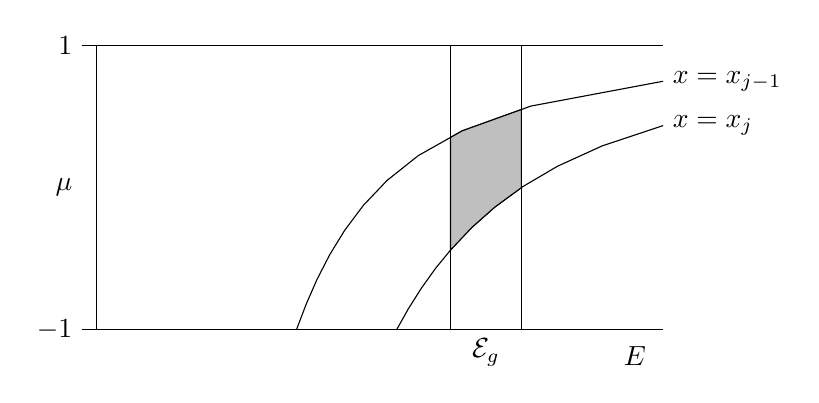
\begin{tikzpicture} [scale=1.8]
% the axes and quadrature box
  \draw(-0.1, -1) -- (4, -1);
  \draw(0, -1) -- (0, 1);
  \draw(-0.1, 1) -- (4, 1);
  \draw(2.5, -1) -- (2.5, 1);
  \draw(3, -1) -- (3, 1);
% x = constant curves
% E' = 2/sqrt{1 - mu}
\draw( 1.4142 , -1.0 ) --
( 1.4805 , -0.825 ) --
( 1.5570, -0.65 ) --
( 1.6468 , -0.475 ) --
( 1.7541, -0.3 ) --
( 1.8856, -0.125 ) --
( 2.0520, 0.05 ) --
( 2.2718, 0.225 ) --
( 2.5820, 0.4 ) --
( 3.0679, 0.575 ) --
( 4.0 , 0.75 );
% E' = 3/sqrt{1 - mu}
\draw( 2.1213, -1.0 ) --
( 2.2019, -0.85625 ) --
( 2.2925, -0.7125 ) --
( 2.3952, -0.56875 ) --
( 2.5131, -0.425 ) --
( 2.6504, -0.28125 ) --
( 2.8128, -0.1375 ) --
( 3.0094 , 0.00625 ) --
( 3.2540, 0.15 ) --
( 3.5698, 0.2938 ) --
( 4.0 , 0.4375 );
% integration region
\filldraw[fill = gray!50] (2.5000, -0.4410) --
( 2.6504, -0.28125 ) --
( 2.8128, -0.1375 ) --
(3.0000, -0.0006) --
(3.0000, 0.5505) --
( 2.5820, 0.4 ) --
( 2.5000, 0.3537) -- cycle;
% labels
  \node[left] at(-0.1, -1){$-1$};
  \node[left]  at(-0.1, 1){$1$};
  \node[left]  at(-0.1, 0){$\mu$};
  \node[below] at(2.75, -1){$\calE_g$};
  \node[below]  at(3.8, -1.05){$E$};
  \node[right] at(4, 0.75){$x = x_{j-1}$};
  \node[right]  at(4, 0.4375){$x = x_j$};
\end{tikzpicture}
\caption{Domain of integration for whole-atom scattering}
\label{Fig:coherent}
\end{center} 

\end{figure}

The domain of integration for Eq.~(\ref{Ien-whole-atom-intE}) is
shown in Figure~\ref{Fig:coherent}.  The curves for $x = x_{j-1}$ and $x = x_j$
are obtained from Eq.~(\ref{def-x-MeV}), and for $x_{j-1} \le x \le x_j$
the region of integration is bounded by these two curves and
lies within the $\calE_g$ energy bin.  This region is shaded gray in
Figure~\ref{Fig:coherent}.

\subsection{A programming detail}
Because of the $\sqrt{1 - \mulab}$ singularity in Eq.~(\ref{def-x-MeV}),
the default method for evaluating integrals with respect to $\mulab$ in 
this section is adaptive quadrature based on first-order Gaussian quadrature
for
\begin{equation}
  \int_a^b d\mulab \, F(\mulab) \sqrt{ 1 - \mulab}.
 \label{Gauss-quad-half}
\end{equation}
This method is used for integration over $\mulab$ in 
Eqs.~(\ref{total-sigma-whole-atom}) and~(\ref{Ien-whole-atom-intE}).

The default method for integration over incident energy $E$ in
Eq.~(\ref{Ien-whole-atom-intE}) is second-order adaptive Gaussian
quadrature.

\subsection{The input file for coherent scattering}
For coherent scattering, the reaction identifier in Section~\ref{data-model} 
is\\
  \Input{Process: coherent scattering}{}\\
and the data are always in the laboratory frame\\
  \Input{Product Frame: lab}{}

The quadrature methods with respect to $\mulab$ and $E$
in Eq.~(\ref{Ien-whole-atom-intE}) may be set independently
using the commands of Section~\ref{Sec:QuadratureMethods}.
The defaults are\\
    \Input{mu quadrature method:}{square root}\\
    \Input{Ein quadrature method:}{adaptive}\\
The quadrature method specified for $\mulab$ also applies to the computation of
the cross section in Eq.~(\ref{total-sigma-whole-atom}).

In \xendl\ the values of $x$ in Eq.~(\ref{def-x}) are given in units of
$\text{\AA}^{-1}$, and the \gettransfer\ code converts $x$ to energy using
the factor $ch$.  This conversion must be to the units used for the
energy bin boundaries in Sections~\ref{Ein-bins} and~\ref{Eout-bins}.
The conversion factor from $\text{\AA}^{-1}$
to energy is set as described in 
Section~\ref{Sec:cm-to-Mev}.

The value of the Thompson scattering cross section $\sigma_T$ in
Eq.~(\ref{sigma-whole-atom}) specified as discussed in
Section~\ref{Sec:Thompson-xs}.

Section~\ref{model-info} of the input file contains the information required
for calculation of the differential cross section in Eq.~(\ref{sigma-whole-atom}).
The values of the coherent form factor $F_F(x)$ are
input using\\
    \Input{Form factor: n = $n$}{}\\
    \Input{Interpolation:}{list interpolation flag}\\
followed by $n$ pairs of values of $x$ and $F_F(x)$.  The interpolation
flag is one for simple lists as in Section~\ref{interp-flags-list}.

The  real anomalous form factor $F_R(E)$ and 
imaginary anomalous form factor $F_I(E)$ are input analogously\\
    \Input{anomalous real form factor: n = $n$}{}\\
    \Input{Interpolation:}{list interpolation flag}\\
followed by $n$ pairs of values of $E$ and $F_R(E)$, and\\
    \Input{anomalous imaginary form factor: n = $n$}{}\\
    \Input{Interpolation:}{list interpolation flag}\\
followed by $n$ pairs of values of $E$ and $F_I(E)$.

An input file for coherent scattering with $x$ values to
be converted from $\text{\AA}^{-1}$ to eV
is as follows.\\
    \Input{Process: coherent scattering}{}\\
    \Input{Product Frame: lab}{}\\
   \Input{inverseWaveLengthToEnergyFactor: 12398.4190576}{}\\
    \Input{ThompsonScattering: 0.6652448}{}\\
    \Input{\# Data section}{}\\
    \Input{Form factor: n = 1272}{}\\
    \Input{Interpolation: lin-lin}{}\\
   \Input{ \indent 0.000000000000e+00  8.000000000000e+00}{}\\
 \Input{ \indent 1.000000000000e-03  8.000000000000e+00}{}\\
 \Input{ \indent 5.000000000000e-03  7.997400000000e+00}{}\\
 \Input{ \indent 6.250000000000e-03  7.995640000000e+00}{}\\
 \Input{ \indent 7.187500000000e-03  7.994550000000e+00}{}\\
   \Input{ \indent  }{$\cdots$}\\
 \Input{ \indent 1.000000000000e+09  7.999700000000e-29}{}\\
        \Input{Anomalous real form factor: n = 253}{}\\
    \Input{Interpolation: lin-lin}{}\\
    \Input{ \indent   1.000000000000e+00 -8.001506000000e+00}{}\\
   \Input{ \indent 3.000000000000e+00 -8.012308000000e+00}{}\\
    \Input{ \indent 8.367019000000e+00 -7.916407000000e+00}{}\\
    \Input{ \indent 9.300337000000e+00 -7.564924000000e+00}{}\\
   \Input{ \indent  9.624912000000e+00 -7.096145000000e+00}{}\\
   \Input{ \indent  }{$\cdots$}\\
  \Input{ \indent 1.000000000000e+07 -4.100212000000e-03}{}\\
    \Input{Anomalous imaginary form factor: n = 255}{}\\
    \Input{Interpolation: lin-lin}{}\\
    \Input{ \indent   1.000000000000e+00  0.000000000000e+00}{}\\
  \Input{ \indent3.000000000000e+00  0.000000000000e+00}{}\\
  \Input{ \indent9.030040000000e+00  0.000000000000e+00}{}\\
  \Input{ \indent9.871915000000e+00  0.000000000000e+00}{}\\
  \Input{ \indent9.913590000000e+00  3.647675000000e-01}{}\\
  \Input{ \indent9.920512000000e+00  4.548976000000e-01}{}\\
   \Input{ \indent  }{$\cdots$}\\
   \Input{ \indent1.000000000000e+07  3.311053000000e-07}{}

\section{Compton scattering}
This reaction is also called incoherent scattering, and it is
the scattering of a photon by an individual bound electron.
See the reference~\cite{ENDFB}.
The data in \xendl\ give the values
of the scattering factor $S_F(x)$ for discrete values
of the parameter $x$, defined in Eq.~(\ref{def-x})
or, equivalently, in Eq.~(\ref{def-x-MeV}).  

The angular differential cross section for Compton scattering,
$\sigma_I(\mulab \mid E)$,
depends on the ratio, $\kappa$, of the energy, $E$, of the incident photon
to the rest mass, $m_e$, of the electron,
\begin{equation}
  \kappa = \frac{E}{m_e}.
  \label{Compton-relative-E}
\end{equation}
In terms of $\kappa$ and $x$, the Compton differential cross section is
\begin{equation}
  \sigma_I(\mulab \mid E) =
    \frac{3 \sigma_T S_F(x)}{ 8[ 1 + \kappa(1 - \mulab)]^2 }
    \left[
      1 + \mulab^2 + \frac{\kappa^2 (1 - \mulab)^2}{1 + \kappa(1 - \mulab)}
    \right].
  \label{Compton-xs}
\end{equation}
Here, $\sigma_T$ is again the Thompson scattering coefficient, and the
units of $\sigma_I(\mulab \mid E)$ are barns per unit cosine.
In Eq.~(\ref{Compton-xs}) the scattering factor $S_F(x)$ accounts
for the deviation from the Klein-Nishina formula due to the fact
that the electrons are bound.
Just as for coherent scattering, the cross section for Compton
scattering is given by
\begin{equation}
  \sigma( E) = \int_{-1}^1 d\mulab \, \sigma_I(\mulab \mid E).
  \label{Compton-sigma}
\end{equation}

The calculation in \gettransfer\ of the energy $\Elab'$ of the outgoing photon
from Compton scattering is actually inconsistent.  On the one hand, the formula
Eq.~(\ref{Compton-xs}) for the differential cross section takes
into account the fact that the scattering is from bound electrons.
For the computation of $\Elab'$, however,
the approximation is made that the electron is
initially free and stationary.
This is a discrete two-body reaction,
and conservation of energy and momentum yields the result that
\begin{equation}
  \Elab' = \frac{E}{1 + \kappa(1 - \mulab)}.
  \label{Compton-Eout}
\end{equation}
Therefore, for Compton scattering the kernel $K(\Elab', \mulab \mid E)$ 
in Eq.~(\ref{def_pi}) takes the form
\begin{equation}
   K(\Elab', \mulab \mid E) = w(E) \sigma_I(\mulab \mid E) \,
     \delta\left(
         \Elab' - \frac{E}{1 + \kappa(1 - \mulab)}
     \right).
  \label{K-Compton}
\end{equation}

Upon inserting the kernel Eq.~(\ref{K-Compton}) into Eq.~(\ref{Ien}),
the computation of energy-preserving transfer matrices
for Compton scattering requires evaluation of the integrals
\begin{multline}
    \Ien_{gh,\ell} =
     \int_{\calE_g} dE \,  w(E)
     \int_{\calE_h' } d\Elab' \, \int_{\mulab} d\mulab  \, 
     P_\ell ( \mulab ) \, \sigma_I(\mulab \mid E)
      \widetilde \phi_\ell(E) \\
      \delta \left(
         \Elab' - \frac{E}{1 + \kappa(1 - \mulab)}
     \right)\Elab'.
  \label{Ien-Compton}
\end{multline}
After integrating over $\Elab'$, it is found that
\begin{equation}
    \Ien_{gh,\ell} =
     \int_{\calE_g} dE \, E  w(E) \widetilde \phi_\ell(E) \,
     \int_{\mulab} d\mulab  \,  
         \frac{P_\ell ( \mulab ) \sigma_I(\mulab \mid E)}{1 + \kappa(1 - \mulab)}.
  \label{Ien-Compton-intE}
\end{equation}
As in coherent scattering, the default quadrature method for integration
with respect to $\mulab$ in Eqs.~(\ref{Compton-sigma}) and~(\ref{Ien-Compton-intE})
is first-order 
Gaussian quadrature for the weighted integral Eq.~(\ref{Gauss-quad-half}).

\begin{figure}
% domain of integration for Compton scattering
\begin{center}
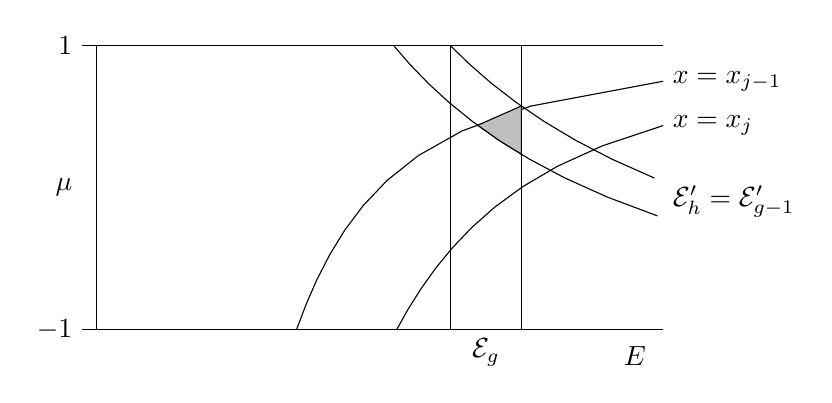
\begin{tikzpicture} [scale=1.8]
% the axes and quadrature box
  \draw(-0.1, -1) -- (4, -1);
  \draw(0, -1) -- (0, 1);
  \draw(-0.1, 1) -- (4, 1);
  \draw(2.5, -1) -- (2.5, 1);
  \draw(3, -1) -- (3, 1);
% x = constant curves
% E' = 2/sqrt{1 - mu}
\draw( 1.4142 , -1.0 ) --
( 1.4805 , -0.825 ) --
( 1.557 , -0.65 ) --
( 1.6468 , -0.475 ) --
( 1.7541 , -0.3 ) --
( 1.8856, -0.125 ) --
( 2.052 , 0.05 ) --
( 2.2718 , 0.225 ) --
( 2.582 , 0.4 ) --
( 3.0679, 0.575 ) --
( 4.0 , 0.75 );
% E' = 3/sqrt{1 - mu}
\draw( 2.1213 , -1.0 ) --
( 2.2019 , -0.85625 ) --
( 2.2925, -0.7125 ) --
( 2.3952 , -0.56875 ) --
( 2.5131 , -0.425 ) --
( 2.6504 , -0.28125 ) --
( 2.8128 , -0.1375 ) --
( 3.0094 , 0.00625 ) --
( 3.254 , 0.15 ) --
( 3.5698 , 0.29375 ) --
( 4.0 , 0.4375 );
% outgoing energy bin
\draw( 3.9388, 0.0667 ) --
( 3.6396, 0.2 ) --
( 3.3826 , 0.3333 ) --
( 3.1595 , 0.4667 ) --
( 2.9640 , 0.6 ) --
( 2.7913 , 0.7333 ) --
( 2.6376, 0.8667 ) --
( 2.5 , 1.0 );
\draw( 3.9598, -0.2 ) --
( 3.6050, -0.06667 ) --
( 3.3086, 0.06667 ) --
( 3.0573, 0.2 ) --
( 2.8414 , 0.3333 ) --
( 2.654, 0.4667 ) --
( 2.4898, 0.6 ) --
( 2.3447 , 0.7333 ) --
( 2.2156, 0.8667 ) --
( 2.1 , 1.0 );
% quadrature region
\filldraw[fill = gray!50]  (2.6920, 0.4396) --
(3.0000, 0.5755) --
(3.0000, 0.2354) --
(2.8414 , 0.3333 ) -- cycle;
% labels
  \node[left] at(-0.1, -1){$-1$};
  \node[left]  at(-0.1, 1){$1$};
  \node[left]  at(-0.1, 0){$\mu$};
  \node[below] at(2.75, -1){$\calE_g$};
  \node[below]  at(3.8, -1.05){$E$};
  \node[right] at(4, 0.75){$x = x_{j-1}$};
  \node[right]  at(4, 0.4375){$x = x_j$};
  \node[right]  at(4, -0.1){$\calE'_h = \calE'_{g-1}$};
\end{tikzpicture}
\caption{Domain of integration for Compton scattering}
\label{Fig:Compton}
\end{center} 

\end{figure}

Because of the relation Eq.~(\ref{Compton-Eout}) between the energies
of the incident and outgoing photons, the range of integration in 
Eq.~(\ref{Ien-Compton-intE}) has an extra degree of complexity in
comparison with Eq.~(\ref{Ien-whole-atom-intE}).  In particular,
the presence of the 
$\delta$-function in Eq.~(\ref{Ien-Compton}) constrains $E$ and
$\mulab$ so that $\Elab'$ is in the $\calE_h'$ energy bin.  Figure~\ref{Fig:Compton}
shows the geometry in the case of down-scattering by one
energy group, $\calE_h' = \calE'_{g-1}$.  In Figure~\ref{Fig:Compton} the curves
delimiting the $\calE_h'$ were obtained by rewriting the energy
condition Eq.~(\ref{Compton-Eout}) in the form
$$
  E = \frac{\Elab'}{1 - (1 - \mulab)\Elab'/m_e}
$$
and taking the top and bottom of the
$\calE_h'$ energy bin as values of~$\Elab'$.  The range of integration in
Eq.~(\ref{Ien-Compton-intE}) is the overlap of the three regions
(1) that determined by the interval $x_i \le x \le x_{i+1}$
of scattering factor data values,
(2) the incident energy bin $E$ in $\calE_g$, and
(3) the outgoing energy bin $\Elab'$ in $\calE_h'$.

\subsection{The input file for Compton scattering}
The reaction identifier in Section~\ref{data-model} for
Compton scattering is\\
  \Input{Process: Compton scattering}{}\\
and the data is always in the laboratory frame\\
  \Input{Product Frame: lab}{}

This default quadrature methods with respect to $\mulab$ 
and $E$ in Eq.~(\ref{Ien-Compton-intE}) are\\
    \Input{mu quadrature method:}{square root}\\
    \Input{Ein quadrature method:}{adaptive}\\
The quadrature method specified for $\mulab$ also applies to the computation of
the cross section in Eq.~(\ref{Compton-sigma}).  It is possible
to override these choices as explained in
Section~\ref{Sec:QuadratureMethods}.

As in coherent scattering, the values of $x$ used for Compton
scattering in \xendl\ are in units of $\text{\AA}^{-1}$, so these are
converted to energy units as in Section~\ref{Sec:cm-to-Mev}.  This
conversion must be to the units used for the energy bin boundaries in
Sections~\ref{Ein-bins} and~\ref{Eout-bins}.

Specification of the Thompson scattering cross section $\sigma_T$
in Eq.~(\ref{Compton-xs}) is as in Section~\ref{Sec:Thompson-xs}.
The value $m_e$ of the rest mass of the electron used in
Eq.~(\ref{Compton-relative-E}) is set as
in Section~\ref{Sec:electron-mass}, and it must be given
in the units used for the energy bin boundaries.

Section~\ref{model-info} of the input file contains the value of the
scattering factor $S_F(x)$ for various values of~$x$.  The format is\\
    \Input{ScatteringFactorData: n = $n$}{}\\
    \Input{Interpolation:}{list interpolation flag}\\
followed by $n$ pairs of values of $x$ and $S_F(x)$.    The interpolation
flag is one for simple lists as in Section~\ref{interp-flags-list}.

An input file for Compton scattering with units of $x$
to be converted from $\text{\AA}^{-1}$ to eV is as follows.\\
    \Input{Process: Compton scattering}{}\\
    \Input{Product Frame: lab}{}\\
   \Input{inverseWaveLengthToEnergyFactor: 12398.4190576}{}\\
    \Input{ThompsonScattering: 0.6652448}{}\\
    \Input{Electron mass: 511000}{}\\
    \Input{ScatteringFactorData: n = 453}{}\\
    \Input{Interpolation: lin-lin}{}\\
     \Input{ \indent 0.000000000000e+00  0.000000000000e+00}{}\\
  \Input{ \indent 1.000000000000e-07  1.100000000000e-12}{}\\
  \Input{ \indent 1.059602649007e-07  1.235033551160e-12}{}\\
  \Input{ \indent 1.126760563380e-07  1.396548303908e-12}{}\\
  \Input{ \indent 1.163636363636e-07  1.489454545455e-12}{}\\
\Input{ \indent }{$\cdots$}\\
 \Input{ \indent 1.000000000000e+09  8.000000000000e+00}{}
 

\chapter{Usage of \gettransfer}
\label{Sec:usage}
The command to run \gettransfer\ is\\
  \Input{\gettransfer\ [-inputOption]}{InputFile}\\
The input options are described in Section~\ref{Sec:usage-optional} below.
Most of them may be specified either in the input file or on the
command line, and command line options override those given in the
input file.  For example, to get output with 9 significant figures,
the command line could be\\
\Input{getTransferMatrix\ -datafield\_precision 9}{InputFile}\\
Alternatively, one may insert the line\\
   \Input{datafield\_precision: 9}{}\\
into the input file.  Note the presence of the colon in this line.
The format for identification of data in the input file is\\
  \Input{data identifier:}{value}

For most types of data, the units of energy are arbitrary, but they
must be consistent.  In particular, rest masses of particles must
be in the same units as the energy bins.  As mentioned in the
individual sections on the data, some models require that
energies be given in MeV.

\section{Output file}
The default name of the output file is \texttt{utfil}.  
It may be changed on the command line with\\
  \Input{-output}{OutputFile}\\
It may also be changed with the
line\\
  \Input{output:}{OutputFile}\\
  in the input file.

\section{Form of the input file}
The first line of the input file must be\\
  \Input{xndfgenTransferMatrix: version 1.0}{}\\
This line is followed by information common to all data models.
The file closes with data specific to the particular data model.
Blank lines are ignored.
  
\subsection{Comments}
Comments may be included in the input file in either if two forms.\\
 \Input{Comment:}{This comment is printed to the output file.}\\
 \Input{\#}{On a line, anything after a pound sign is ignored.}\\
 For example, the input file usually contains a comment identifying the
 particles involved in the reaction, e.g.,\\
   \Input{Comment: n1 + C12 --> n1 + C12 outgoing data for n1}{}
 
\subsection{Parallel computing}
The \gettransfer\ code may be compiled to run in parallel if
\textsf{OpenMP} is available on your computer.  In fact, the
default \textsf{Makefile} uses \textsf{OpenMP}.  Compile with
\textsf{Makefile\_serial} to obtain serial code.  

For the parallel code, the number of threads is set to $n$ by the
line\\
  \Input{num\_threads:}{$n$}\\
in the input file.  The default is $n = 0$, which causes the computer
to choose the number of threads.  If the specified $n$ is larger than
the number of available threads, then the code runs on the threads
available.

The parallel code may be forced to run in serial mode by
the command line  option\\
 \Input{-num\_threads~1} {}\\
or by inclusion of\\
 \Input{num\_threads:~1}{}\\
in the input file.

 \subsection{Interpolation flags} \label{interp-flags}
The identifiers for the standard interpolation methods
 given in Section~\ref{Sec:1d-interp} are\\
    \Input{flat}{for histograms}\\
   \Input{lin-lin}{for linear-linear}\\
   \Input{lin-log}{for linear-log}\\
   \Input{log-lin}{for log-linear}\\
   \Input{log-log}{for log-log}\\
The identifiers are incorporated in different ways into the interpolation
flags for simple lists such as reaction cross sections, for probability densities,
and for the Kalbach-Mann $r$ and~$a$ parameters.  The complete
identifiers for the interpolation of the various types of tabulated data are as follows.

\subsubsection{Interpolation flags for simple lists}\label{interp-flags-list}
 For simple lists of data such as $\{E, M\}$ for particle multiplicity~$M$ at
 incident energy~$E$, the interpolation flags are\\
   \Input{Interpolation: }{identifier}\\
with one of the identifiers above.  For example, the command\\
   \Input{Interpolation: lin-lin}{}\\
specifies linear-linear interpolation.

\subsubsection{Interpolation flags for probability densities}\label{interp-flags-probability}
For probability density tables 
\begin{equation}
  \{x, y, \pi(y \mid x) \},
 \label{xypi-data}
\end{equation}
the interpolation
method with respect to~$x$ as discussed in Section~\ref{Sec:2d-interp}
is identified by\\
   \Input{$x$ interpolation:}{identifier interpolation-flag}\\
where the identifier is one of those for simple lists and the
interpolation flag here is one of\\
   \Input{direct }{for direct interpolation with extrapolation}\\
   \Input{unitbase }{for unit-base interpolation}\\
   \Input{cumulativepoints }{for interpolation by cumulative points}\\
Thus, a table of probability densities of outgoing energies $\pi( E' \mid E)$ may
be marked\\
   \Input{Incident energy interpolation: lin-lin cumulativepoints}{}\\
to indicate that interpolation with respect to incident energy~$E$ is to be done
using linear-linear cumulative points as in Section~\ref{Sec:cumProb}.

The method for interpolation of the data in Eq.~(\ref{xypi-data}) with
respect to $y$ is specified by\\
   \Input{$y$ interpolation:}{identifier}\\
with an identifier as in a simple list.  For example, the command\\
   \Input{Outgoing energy interpolation: flat}{}\\
specifies histogram interpolation with respect to the energy of
the outgoing particle.

\subsubsection{Interpolation flags for unscaled interpolation of
Kalbach-Mann data}\label{interp-flags-Kalbach-r}
The methods of interpolation of tables for the Kalbach-Mann 
parameters $r(E', E)$ and $a(E', E)$ with respect to the energy~$E$
of the incident particle are discussed in Section~\ref{Sec:Kalbach-r-interp}.
The options for interpolation flags are\\
   \Input{Incident energy interpolation:}{identifier \texttt{unscaleddirect}}\\
   \Input{Incident energy interpolation:}{identifier \texttt{unscaledunitbase}}\\
   \Input{Incident energy interpolation:}{identifier \texttt{unscaledcumulativepoints}}\\
where the identifier is one of those for simple lists. 
For example, the command denoting linear-linear unscaled unit-base interpolation
with respect to incident energy is\\
   \Input{Incident energy interpolation: lin-lin unscaledunitbase}{}

The method for interpolation of tables of Kalbach-Mann $r$ and~$a$ parameters
with respect to outgoing energy~$E$ is specified by\\
   \Input{Outgoing energy interpolation:}{identifier}\\
with an identifier as in a simple list.  For example, the comand\\
   \Input{Outgoing energy interpolation: flat}{}\\
specifies histogram interpolation with respect to the energy of
the outgoing particle.

\section{Information used by all data models}
The following information is required, but the order
is arbitrary.

\subsection{The data model} \label{data-model}
Identification of the data model.\\
  \Input{Process:}{Identifier of the type of data}\\
These identifiers are specified in the previous sections.

\subsection{Incident energy groups}\label{Ein-bins}
The boundaries of the incident energy groups.\\
  \Input{Projectile's group boundaries: n = $n$}{}\\
This is followed by the $n$ values the incident energy bin
boundaries.  Thus, in units of eV this section may take the form\\
  \Input{Projectile's group boundaries: n = 88}{}\\
  \Input{  1.306800000000e-03  2.090800000000e-02  1.306800000000e-01}{}\\ 
  \Input{  3.345300000000e-01  1.176100000000e+00  2.090800000000e+00}{}\\
   \Input{ \indent $\cdots$}{}\\
  \Input{  2.000000000000e+07 }{}

\subsection{Outgoing energy groups}\label{Eout-bins}
The boundaries of the outgoing energy groups.\\
  \Input{Product's group boundaries: n = $n$}{}\\
This is followed by the $n$ values the outgoing energy bin
boundaries.  The units must be the same as for the incident
energy groups.  A sample input given in eV is\\
  \Input{Product's group boundaries: n = 88}{}\\
  \Input{  1.306800000000e-03  2.090800000000e-02  1.306800000000e-01}{}\\ 
  \Input{  3.345300000000e-01  1.176100000000e+00  2.090800000000e+00}{}\\
   \Input{ \indent $\cdots$}{}\\
  \Input{  2.000000000000e+07 }{}

\subsection{Frames of reference}\label{Reference-frame}
The energy $E$ of the incident particle must be given in the laboratory frame,
as indicated by the command\\
  \Input{Projectile Frame: lab}{}\\
For the outgoing particle, the energy $E'$ and direction cosine~$\mu$
may be given in the laboratory frame with\\
  \Input{Product Frame: lab}{}\\
or the center-of-mass frame as\\
  \Input{Product Frame: CenterOfMass}{}

\subsection{Relativistic kinetics}\label{Sec:relativistic}
For discrete 2-body reactions, 
the code may use either Newtonian or relativistic mechanics in its
computations.  The command to control this option is\\
  \Input{kinetics: Newtonian}{}\\
or\\
  \Input{kinetics: relativistic}{}\\
The default is \texttt{Newtonian} except when the emitted particle is a gamma.

\subsection{Approximate flux}
The Legendre coefficients $\widetilde \phi_\ell(E)$ used as weights in
the integrals Eqs.~(\ref{Inum}) and~(\ref{Ien}).\\
  \Input{Fluxes: n = $n$}{}\\
  \Input{Interpolation:}{interpolation flag}\\
Here, $n$ is the number of incident energies $E$, and
the interpolation flag is one of those for simple lists, Section~\ref{interp-flags-list}.
Note that because of the scaling performed in Eqs.~(\ref{cons_num})
and~(\ref{cons_en}), the units of $\widetilde \phi_\ell(E)$
are arbitrary, but barns are most common.  The computed transfer matrix is unchanged if
$\widetilde \phi_\ell(E)$ is multiplied by a constant.

For each incident energy, the input file has a block specifying
the Legendre coefficients  given as\\
 \Input{ Ein: $E$:}{  n = $n$}\\
and $\widetilde \phi_\ell(E)$ for $n = 0$, 1, \ldots , $n - 1$.
The incident energy $E$ must be in the same units as the
energy groups.
The number of Legendre coefficients given here need not be
consistent with the Legendre order $L$ of the computed transfer
matrix as specified in Section~\ref{Sec:LegendreOrder}.  
If $n - 1 < L$, then the {\gettransfer} code sets
$$
  \widetilde \phi_\ell(E) = \widetilde \phi_{n - 1}(E)
  \quad \text{for $\ell = n$, $n+1$, \ldots, $L$.}
$$

A sample input with $E$ in eV and with all Legendre coefficients
the same is\\
  \Input{Fluxes: n = 2}{}\\
  \Input{Interpolation: lin-lin}{}\\
  \Input{ Ein: 0:  n = 1}{}\\
  \Input{  \indent 8.500000000000e+01}{}\\
  \Input{ Ein: 2.100000000000e+07:  n = 1}{}\\
  \Input{  \indent 8.500000000000e+01}{}

\subsection{Reaction cross section}
As explained in Section~\ref{Sec:gamma-in}, the cross sections for coherent photon
scattering and Compton scattering are computed from the data.
Reaction cross sections are required for all other data models.\\
  \Input{Cross section: n = $n$}{}\\
  \Input{Interpolation:}{interpolation flag}\\
Here, $n$ is the number of pairs $\{E, \sigma(E)\}$,
and the interpolation flag is one of those for simple lists,
Section~\ref{interp-flags-list}.  This is
followed by $n$ pairs of incident energy~$E$ and reaction cross
section~$\sigma( E )$.

A sample of such data with energies in MeV is given by\\
 \Input{Cross section: n = 22}{}\\
 \Input{Interpolation: lin-lin}{}\\
  \Input{  \indent  7.78148000e+00  0.00000000e+00}{}\\
  \Input{  \indent  7.80000000e+00  4.40157000e-04}{}\\
  \Input{  \indent  8.00000000e+00  1.13781000e-02}{}\\
  \Input{  \indent  8.50000000e+00  6.96097100e-02}{}\\
  \Input{  \indent }{ $\cdots$}\\
  \Input{  \indent  2.00000000e+01  9.17094100e-01}{}

\subsection{Multiplicity}
The multiplicity of the outgoing particle must be given if it is
different from~1.  The format is\\
  \Input{Multiplicity: n = $n$}{}\\
  \Input{Interpolation:}{interpolation flag}\\
followed by $n$ pairs $\{E, M(E)\}$.  
The interpolation flag is one of those for simple lists,
Section~\ref{interp-flags-list}.  The units of incident energy
$E$ must be the same as for the energy groups.  
For example, with $E$ in MeV, an $(n, 2n)$ reaction
would typically have\\
  \Input{Multiplicity: n = 2}{}\\
  \Input{Interpolation:}{flat}\\
  \Input{0.0    2.0}{}\\
  \Input{20.0  2.0}{}


\subsection{Model weight}
The model weight $w_r(E)$ is used in the formation of the reaction
kernel $\calK_r(E', \mu \mid E)$ in Eq.~(\ref{def_pi}) and is
discussed in Section~\ref{Sec:model-weight}.  Its value
is usually~1 over the entire range of incident energies in the cross
section data.  If this is not the case, then the model weight is input as\\
  \Input{Weight: n = $n$}{}\\
  \Input{Interpolation: flat}{}\\
followed by $n$ pairs $\{E, w(E)\}$.   For example, the weight
$$
  w(E) = \begin{cases}
    0 & \text{for $0 \le E < 6$,}\\
    1 & \text{for $6 \le E \le 20$,}\\
  \end{cases}
$$
may be specified using the input\\
   \Input{Weight: n = 3}{}\\
  \Input{Interpolation: flat}{}\\
  \Input{0.0    0.0}{}\\
  \Input{6.0    1.0}{}\\
  \Input{20.0  1.0}{}
  
\section{Optional flags, output information}
\label{Sec:usage-optional}
The following options control the output of \gettransfer.
All of them may also be input as command line options.

\subsection{Legendre order of the output}\label{Sec:LegendreOrder}
The Legendre order of the matrices Eqs.~(\ref{Inum}) and~(\ref{Ien})
computed by \gettransfer\ is set by the command\\
  \Input{outputLegendreOrder: n = $L$}{}\\
The default is $L = 3$.

\subsection{Numerical precision of the output}
The number of significant figures for the output data is set by\\
  \Input{datafield\_precision: n = $n$}{}\\
The default is $n = 8$.

\subsection{Conservation flag}\label{Sec:conserveFlag}
This flag determines whether the \gettransfer\ code computes integrals
   Eq.~(\ref{Inum}) for the number-conserving transfer matrix,
   integrals  Eq.~(\ref{Ien}) for the energy-conserving matrix, or both.
   The options are\\
   \Input{Conserve: number}{}\\
for the integrals Eq.~(\ref{Inum})\\
   \Input{Conserve: energy}{}\\
for the integrals Eq.~(\ref{Ien})\\
   \Input{Conserve: both}{}\\
for the both integrals.  The default is \texttt{both} for most types of data.

\subsection{Consistency check}
If the integrals Eq.~(\ref{Inum}) for the number-preserving transfer matrix
are computed, it is possible to check the consistency as in Eq.~(\ref{rowSum}).
With the option\\
  \Input{check\_row\_sum: true}{}\\
both sides of Eq.~(\ref{rowSum}) are printed, along with their differences
and relative differences.  This information is not printed if the option is \texttt{false}.
The default is \texttt{false}.

To scale the integrals Eq.~(\ref{Inum}) so as to enforce the identity
Eq.~(\ref{rowSum}), use the option\\
  \Input{scale\_rows: true}{}\\
In this case, the integrals Eq.~(\ref{Ien}) are also scaled.  The default
is \texttt{true}, scale the integrals.

\section{Optional inputs, quadrature methods}\label{Sec:QuadratureMethods}
For the integrals Eqs.~(\ref{Inum}) and~(\ref{Ien}) and their equivalents
in the center-of-mass frame, the quadrature methods may be set
by commands of the form\\
  \Input{\textrm{Variable} quadrature method:}{Method}\\
The `Variable' in this line is any of the following.\\
  \Input{Ein}{for integrals with respect to incident energy~$E$,}\\
  \Input{Eout}{for integrals with respect to outgoing energy~$\Elab'$ or~$\Ecm'$,}\\
  \Input{mu}{for integrals with respect to direction cosine~$\mulab$ of ~$\mucm$.}\\
  \Input{-}{Omission of this parameter gives the same quadrature method for all integrals.}\\
The options for the `Method' in the command to set the quadrature method
are\\
  \Input{adaptive}{for adaptive 2nd-order Gaussian quadrature,}\\
  \Input{square root}{for adaptive 1st-order Gaussian quadrature with weight $\sqrt{1 - \mu}$,}\\
  \Input{Gauss2}{for non-adaptive 2nd-order Gaussian quadrature,}\\
  \Input{Gauss4}{for non-adaptive 4th-order Gaussian quadrature,}\\
  \Input{Gauss6}{for non-adaptive 6th-order Gaussian quadrature.}\\
The default for most data models is\\
  \Input{quadrature method: adaptive}{}\\
to use adaptive 2nd-order Gaussian  quadrature for all integrals.
The exceptions are\\
  \Input{mu quadrature method: square root}{}\\
for the integrals over direction cosine $\mulab$ with data for
coherent scattering and Compton scattering.  The non-adaptive options
are primarily used in debugging.

\section{Optional inputs, numerical tolerances}
The user may reset the tolerances for convergence of the adaptive quadrature
and for determination of the equality of two floating-point numbers.

\subsection{Convergence of adaptive quadrature}
The adaptive quadrature routine produces an estimate $\calI$ of
the integral, along with an estimate $e_\calI$ of the error.  The process of
successive subdivision stops when
$$
  | e_\calI | < \epsilon_a + \epsilon_r | \calI |.
$$
The absolute quadrature tolerance is set by the command\\
  \Input{abs\_quad\_tol:}{$\epsilon_a$}\\
The default is $\epsilon_a = \texttt{1.0e-8}$.  To set the relative
quadrature tolerance, use\\
  \Input{quad\_tol:}{$\epsilon_r$}\\
The default is $\epsilon_r = \texttt{1.0e-4}$. 

There is also a limit on the total number of intervals used in
adaptive quadrature\\
  \Input{max\_divisions: n = $n$}{}\\
If this limit is exceeded, the adaptive quadrature routine returns
the current estimate and prints a warning that this result may be
inaccurate.

\subsection{Near equality of floating-point numbers}
In comparisons of floating-point numbers $x_1$ and~$x_2$, the code treats 
them as essentially equal if
$$
  | x_1 - x_2 | \le \delta_a + \delta_r \min( | x_1 |, | x_2 | ).
$$
Here, the absolute tolerance $\delta_a$ is set by\\
  \Input{abs\_tol:}{$\delta_a$}\\
The default value is $\delta_a = \texttt{2.0e-14}$ and is appropriate
when energies are measured in MeV.  It should be scaled accordingly,
when other energy units are used.  The relative tolerance
$\delta_r$ is set using\\
  \Input{E\_tol:}{$\delta_r$}\\
The default value is $\delta_r = \texttt{1.0e-9}$.

\section{Physical constants}
The coding for coherent photon scattering and Compton scattering
discussed in Section~\ref{Sec:gamma-in} requires the values of several physical
constants.  These are input as follows.

\subsection{Conversion from $\text{\AA}^{-1}$ to energy}\label{Sec:cm-to-Mev}
In order to convert the energy of photons from inverse wavelength
to energy, multiply by $ch$.  This parameter is set by
the command\\
  \Input{inverseWaveLengthToEnergyFactor:}{$ch$}.

\subsection{Thompson scattering cross section}\label{Sec:Thompson-xs}
The Thompson scattering cross section $\sigma_T$ in 
Eqs.~(\ref{sigma-whole-atom}) and~(\ref{Compton-xs}) is
set by\\
  \Input{ThompsonScattering:}{$\sigma_T$}\\
The default value is $\sigma_T = \texttt{0.6652448}$ barns.

\subsection{Electron rest mass}\label{Sec:electron-mass}
The rest mass $m_e$ of the electron in Eq.~(\ref{Compton-relative-E}) is
set by the command\\
  \Input{electron mass:}{$m_e$}.

\subsection{Neutron rest mass}\label{Sec:neutron-mass}
The rest mass of the neutron $m_n$ is used in Eq.~(\ref{Kalbach-photo})
by the Kalbach-Mann model of photo-nuclear reactions.
Its units are MeV, and its value is set by the command\\
  \Input{m\_neutron:}{$m_n$}\\
Its default value is $m_n = \texttt{939.565653471}\,$MeV.

\section{Errors and warning messages}
These options control the printing of informational messages,
warnings, and fatal errors.  To set which messages are printed,
use the command\\
  \Input{message\_level: n = $n$}{}\\
The effect of this option is:
$$
  \texttt{message\_level} =
    \begin{cases}
       0& \text{print all messages},\\
       1& \text{print only warnings and errors},\\
       2& \text{print only severe errors; these cause exits anyway}.
    \end{cases}
$$
The default value is 0, print all messages.

It is also possible to turn off all messages with the command\\
  \Input{skip\_logging:}{\texttt{true}}\\
The default value is \texttt{false}.

\section{Model-dependent information}\label{model-info}
The remainder of the input file consists of data required by the model. 

\appendix
{ % localize the newcommands
\newcommand{\mzerot}{m_{t,0}}
\newcommand{\mzeroi}{m_{i,0}}
\newcommand{\Ezerot}{m_t}
\newcommand{\Ezeroi}{m_i}
\newcommand{\EzeroR}{m_R}
\newcommand{\Ezeroe}{m_e}
\newcommand{\Tlabin}{T_{i,\textrm{lab}}}
\newcommand{\plabin}{p_{i,\textrm{lab}}}
\newcommand{\Tlabe}{T_{e,\textrm{lab}}}
\newcommand{\plabe}{p_{e,\textrm{lab}}}
\newcommand{\plabea}{p_{e1,\textrm{lab}}}
\newcommand{\plabeb}{p_{e2,\textrm{lab}}}
\newcommand{\plabec}{p_{e3,\textrm{lab}}}
\newcommand{\Tcmi}{T_{i,\textrm{cm}}}
\newcommand{\Tcmt}{T_{t,\textrm{cm}}}
\newcommand{\Tcme}{T_{e,\textrm{cm}}}
\newcommand{\TcmR}{T_{R,\textrm{cm}}}
\newcommand{\pcmi}{p_{i,\textrm{cm}}}
\newcommand{\pcme}{p_{e,\textrm{cm}}}
\newcommand{\pcmea}{p_{e1,\textrm{cm}}}
\newcommand{\pcmeb}{p_{e2,\textrm{cm}}}
\newcommand{\pcmec}{p_{e3,\textrm{cm}}}
%\newcommand{\mucm}{\mu_{\textrm{cm}}}
%\newcommand{\mulab}{\mu_{\textrm{lab}}}

\chapter{Relativistic 2-body problems}
\label{Appendix-relativity}
In this appendix, relativistic 2-body mechanics is examined from the point
of view of computational physics.  That is, the subtraction
nearly equal numbers is avoided as much as is possible.
The analysis starts with a collision of an incident particle with
a stationary target.  This determines the mapping between
the laboratory frame and the center-of-mass frame.  
The appendix closes with a discussion of
emission after the reaction. 

As is customary in discussions of relativity, the units are
such that the speed of light has the value~$c = 1$.

\section{Initial collision}
For this appendix, $E$ is the total energy of
a system
and $p$ its total momentum.  Thus, for a particle with rest mass~$m_0$
and kinetic energy~$T$, it follows that $E = m_0 + T$. 
\textit{The convention $c = 1$ implies that the data must be such that
particle rest masses and kinetic energies must be given in the same units.}
The analysis makes repeated use of the invariance under Lorentz
transformations of the quantity
\begin{equation}
  S_0 = E^2 - p^2.
  \label{spacetime}
\end{equation}

If the system is a single particle
in a frame in which the particle is stationary, then $S_0 = m_0^2$.
Consequently, for a single particle in
any frame Eq.~(\ref{spacetime}) takes the form
\begin{equation}
  m_0^2 = (m_0 + T)^2 - p^2,
 \label{spacetime-1}
\end{equation}
or
\begin{equation}
  p^2  = 2m_0 T + T^2.
  \label{one-p}
\end{equation}
When it is desired to solve Eq.~(\ref{one-p}) for~$T$ corresponding
to a known value of~$p^2$, it is recommended to use the formula
\begin{equation}
  T = \frac{p^2 }
          {m_0 + \sqrt{ m_0^2 + p^2 }}.
 \label{good-T}
\end{equation}
The relation Eq.~(\ref{good-T}) is computationally more reliable
than the more obvious solution of the quadratic equation Eq.~(\ref{one-p})
$$
  T = -m_0 + \sqrt{ m_0^2 + p^2 }.
$$

Consider the application of Eq.~(\ref{spacetime}) to the system
consisting of a moving incident particle and a target 
at rest in
the laboratory frame.  Suppose that the incident
particle has rest mass $\Ezeroi$ and kinetic
energy $\Tlabin$, and let $\Ezerot$ be the rest mass of the
target.  Then it follows from Eq.~(\ref{one-p})
that the initial laboratory-frame momentum is given by
\begin{equation}
  \plabin^2  = 2\Ezeroi \Tlabin + \Tlabin^2.
 \label{p-lab-in}
\end{equation}
Consequently, for the system of consisting of the two particles
in the laboratory frame, the energy-momentum invariant is
$$
  S = (\Ezerot + \Ezeroi + \Tlabin)^2 -
      ( 2\Ezeroi \Tlabin + \Tlabin^2 ),
$$
This expression simplifies to
\begin{equation}
  S = (\Ezeroi + \Ezerot )^2 + 2\Ezerot \Tlabin.
  \label{S-lab}
\end{equation}

The value of $S$ must be the same when this
system of two particles is considered in the center-of-mass
frame.  Denote the center-of-mass kinetic energy of
the incident particle by $\Tcmi$ and its momentum by~$\pcmi$.
Similarly, let the target have center-of-mass kinetic energy $\Tcmt$, 
and its momentum is~$-\pcmi$.  The energy-momentum invariant
for the system is therefore
\begin{equation}
  S = (\Ezeroi + \Tcmi + \Ezerot + \Tcmt)^2,
 \label{spacetime-cm}
\end{equation}
the square of the total energy of the system in the center-of-mass frame.
By using Eq.~(\ref{spacetime-1}) on each of the particles, it
is possible to rewrite this as
$$
  S = \left(
    \sqrt{\Ezeroi^2 + \pcmi^2 } +
       \sqrt{\Ezerot^2 + \pcmi^2 }
   \right)^2.
$$
Upon solving this equation for $\pcmi^2$, it is found that
\begin{equation}
  \pcmi^2 = \frac{ \left[S - (\Ezeroi^2 + \Ezerot^2)\right]^2 -
                 4 \Ezeroi^2 \Ezerot^2 }
                {4 S }.
  \label{p-cm}
\end{equation}
An expression for $\pcmi^2$ in terms of the
laboratory incident kinetic energy $\Tlabin$ is obtained by substituting
in Eq.~(\ref{p-cm}) the value of $S$ given by Eq.~(\ref{S-lab}),
\begin{equation}
  \pcmi^2 = \frac{\Ezerot^2( 2 \Ezeroi \Tlabin + \Tlabin^2)}
              {(\Ezerot + \Ezeroi )^2 + 2\Ezerot \Tlabin}.
  \label{p-cm-1}
\end{equation}
It follows from Eq.~(\ref{one-p}) that this equation may also
be written as
$$
  \pcmi^2 = \frac{\Ezerot^2 \plabin^2 }
                {(\Ezerot + \Ezeroi )^2 + 2\Ezerot \Tlabin}.
$$

\section{Mapping between frames}
Consider a coordinate system in which the momentum
$\plabin$ of the incident particle is in the direction of
the first spatial axis.  The boost from
the laboratory to the center-of-mass frame then takes the
form
$$
  (E_{\text{cm}}, p_{\text{cm}})^T = R (E_{\text{lab}}, p_{\text{lab}})^T
$$
with the matrix
\begin{equation}
   R =
    \begin{bmatrix}
     \cosh \chi & -\sinh \chi & 0 & 0 \\
     -\sinh \chi & \cosh \chi & 0 & 0 \\
     0  & 0 & 1 & 0 \\
     0  & 0 & 0 & 1
  \end{bmatrix}.
  \label{R-3}
\end{equation}

Upon applying the rotation Eq.~(\ref{R-3}) to the target,
it is found that
$$
     \begin{bmatrix}
        \Ezerot + \Tcmt \\
        -|\pcmi| \\
        0 \\
        0
     \end{bmatrix}
      = R
\begin{bmatrix}
        \Ezerot \\
           0  \\
           0 \\
           0
     \end{bmatrix}.
$$
It follows that
\begin{equation}
   \sinh \chi = \frac{|\pcmi|}{\Ezerot}.
 \label{lab-to-cm}
\end{equation}
By using Eq.~(\ref{p-cm-1}), one may conclude that
\begin{equation}
  \sinh \chi = \frac{\sqrt{ 2 \Ezeroi \Tlabin + \Tlabin^2}}
    {\sqrt{( \Ezerot + \Ezeroi )^2 + 2 \Ezerot \Tlabin }}.
  \label{lab-to-cm-2}
\end{equation}
Note that except for incident gammas, $\Tlabin$ is much smaller
than the rest mass $\Ezeroi$, so that $\chi$ is a
small, positive number.

In the next section of this appendix, for 2-body problems
the center-of-mass energy and momentum of the
emitted particle and residual are determined.  In order to boost these 4-vectors
to the laboratory frame, one may use the inverse of the matrix $R$ in
Eq.~(\ref{R-3}), so that
\begin{equation}
  (E_{\text{lab}}, p_{\text{lab}})^T = R^{-1}(E_{\text{cm}}, p_{\text{cm}})^T
 \label{3d-map}
\end{equation}
with
\begin{equation}
   R^{-1} =
    \begin{bmatrix}
     \cosh \chi & \sinh \chi & 0 & 0 \\
     \sinh \chi & \cosh \chi & 0 & 0 \\
     0  & 0 & 1 & 0 \\
     0  & 0 & 0 & 1
  \end{bmatrix}.
  \label{R-3-inv}
\end{equation}

\subsection{Incident photons}
\label{Sec:photon-in}
When the incident particle is a photon, the boost from the 
center-of-mass frame to the laboratory frame must be determined
relativistically, because the mass of the incident particle is zero
but its momentum is nonzero.

In this case, Eq.~(\ref{p-lab-in}) simplifies to
$$
  | \plabin |  =  \Tlabin,
$$
and Eq.~(\ref{lab-to-cm-2}) becomes
$$
  \sinh \chi = \frac{ \Tlabin}
    {\sqrt{ \Ezerot^2 + 2 \Ezerot \Tlabin }}.
$$
It follows that
$$
  \cosh \chi = \frac{ \Ezerot + \Tlabin}
    {\sqrt{ \Ezerot^2 + 2 \Ezerot \Tlabin }}.
$$



\section{Outgoing particles}
Denote by $\Ezeroe$ the rest mass of the
emitted particle and
$\Tcme$ its kinetic energy in the center-of-mass frame.
The convention in \xendl\ is that the energy~$Q$ of the reaction
is specified by the data, and the rest mass  $\EzeroR$ of the residual
is calculated from
\begin{equation}
  \EzeroR = \Ezerot + ( \Ezeroi - \Ezeroe ) - Q.
 \label{Q-2body}
\end{equation}
Let $\TcmR$ be the kinetic energy of the residual in the center-of-mass frame.
In terms of these variables, the energy-momentum invariant
for the system is the square of the total energy
$$
    S = (\Ezeroe + \Tcme + \EzeroR + \TcmR)^2,
$$
with the same value of $S$ as in Eq.~(\ref{spacetime-cm}).
The argument leading to Eq.~(\ref{p-cm}) shows that the
momentum~$\pcme$ of the emitted particle in the center-of-mass frame
has magnitude given by
\begin{equation}
  \pcme^2 = \frac{ \left[S - (\EzeroR^2 + \Ezeroe^2)\right]^2 -
                 4 \EzeroR^2 \Ezeroe^2 }
                {4 S }.
  \label{p-cm-e}
\end{equation}

It is not a good idea to use Eq.~(\ref{p-cm-e}) in a
computation, because of its subtraction of nearly equal
numbers.  It is therefore desirable to do some algebraic manipulation
in order to mitigate this problem as much as possible.
As a first step, Eq.~(\ref{p-cm-e}) is rewritten in the
form
\begin{equation}
  4 S \pcme^2 = \left[S - (\EzeroR + \Ezeroe)^2\right]
              \left[S - (\EzeroR - \Ezeroe)^2\right].
 \label{p-cm-e-1}
\end{equation}
In this expression, the subtraction of nearly equal
numbers is confined to the first factor on the right-hand
side.  For photon emission the two factors are identical.
An analysis of photon emission later, because it offers some
simplifications.

By using the expression for~$S$ in Eq.~(\ref{S-lab}), one
obtains the relation
$$
  S - (\EzeroR + \Ezeroe)^2 =
  (\Ezerot + \Ezeroi)^2 - (\EzeroR + \Ezeroe)^2  + 2\Ezerot \Tlabin.
$$
In terms of the energy $Q$ of the discrete 2-body reaction
and the parameter
\begin{equation}
  M_T = \Ezerot + \EzeroR + \Ezeroi + \Ezeroe,
 \label{def-M}
\end{equation}
it follows that
$$
    S - (\EzeroR + \Ezeroe)^2 =
     M_T Q + 2\Ezerot \Tlabin.
$$
Consequently, it is seen that Eq.~(\ref{p-cm-e}) may be
replaced by
\begin{equation}
  \pcme^2 = \frac{ (M_T Q +  2\Ezerot \Tlabin )
                 ( M_T Q +  2\Ezerot \Tlabin + 4\EzeroR \Ezeroe)}
                {4 S }.
  \label{p-cm-e-OK}
\end{equation}

\textbf{Remark.}
It is clear from Eq.~(\ref{p-cm-e-OK}) that for endothermic
reactions ($Q < 0$), the threshold occurs when the incident
particle has kinetic energy
$$
  \Tlabin = \frac{-M_T Q}{2\Ezerot}.
$$

In Eq.~(\ref{p-cm-e-OK}) there is subtraction of nearly equal
numbers when the kinetic energy $\Tlabin$ of the incident
particle is just above the threshold in endothermic reactions.
That operation is unavoidable in
the analysis of nuclear reactions. 

Now that $\pcme^2$ has been obtained in Eq.~(\ref{p-cm-e-OK}), one may use
Eq.~(\ref{good-T}) to determine the kinetic energy of the
emitted particle in the center-of-mass frame as
\begin{equation}
  \Tcme = \frac{\pcme^2 }
          {\Ezeroe + \sqrt{ \Ezeroe^2 + \pcme^2 }}.
 \label{T-cm-e}
\end{equation}

\subsection{The boost to the laboratory frame}
It is often desired to determine the kinetic energy~$\Tlabe$
and momentum~$\plabe$ of the emitted particle in the laboratory frame
for given direction cosine~$\mucm$ in the center-of-mass frame.
It is possible to use the boost 
Eq.~(\ref{3d-map}) to determine $\plabe$ as follows.  Recall that
the form of Eq.~(\ref{3d-map}) is determined by the requirement that
the first axis of the coordinate system was chosen parallel to~$\plabin$.
Consequently, one has
$$
  \pcmea = \mucm |\pcme|.
$$
If the orientation of the coordinate system is such that
$$
  \pcmec = 0
  \quad \textrm{and} \quad
  \pcmeb \ge 0,
$$
then
$$
  \pcmeb =  |\pcme| \sqrt{ 1 - \mucm^2}.
$$
The momentum components of the boost Eq.~(\ref{3d-map}) then
take the form
\begin{equation*}
\begin{split}
  \plabea &= (\Ezeroe + \Tcme)\sinh \chi +  \mucm |\pcme| \cosh \chi, \\
  \plabeb &= |\pcme| \sqrt{ 1 - \mucm^2}, \\
  \plabec & = 0.\\
\end{split}
\end{equation*}

The magnitude of the momentum in the laboratory frame is
$$
  |\plabe| = \sqrt{ \plabea^2 + \plabeb^2 + \plabec^2 }.
$$
If $|\plabe| = 0$, the direction cosine $\mulab$ in the laboratory
frame is undetermined.  Otherwise, it is given by
$$
  \mulab = \frac{\plabea}{|\plabe|}.
$$
The kinetic energy $\Tlabe$ is calculated from $|\plabe|$
by using Eq.~(\ref{good-T}).

\subsection{Photon emission}
When the emitted particle is a photon, because $\Ezeroe = 0$,
Eqs.~(\ref{p-cm-e-OK}) and (\ref{T-cm-e}) take the simpler form
$$
  E_{e, \textrm{cm}} = \Tcme = |\pcme| =
   \frac{ M_T Q +  2\Ezerot \Tlabin }
                {2 \sqrt{S} }.
$$
For given direction cosine~$\mucm$ in the center-of-mass frame,
the energy component of the boost Eq.~(\ref{3d-map}) gives the
Doppler shift
$$
   E_{e, \textrm{lab}} = E_{e, \textrm{cm}}
     \left( \cosh \chi + \mucm \sinh \chi \right).
$$
The first component of the momentum of the photon in the laboratory
frame is
$$
  \plabea =  E_{e, \textrm{cm}}
     \left( \sinh \chi + \mucm \cosh \chi \right),
$$
so the direction cosine is
$$
  \mulab = \frac{\sinh \chi + \mucm \cosh \chi}
                {\cosh \chi + \mucm \sinh \chi}.
$$

} % end of this appendix

\chapter{Proof of Assertion~\ref{Sec:assertion8}}
\label{Sec:Appendix-B}
It is proved in this appendix that for a Newtonian boost,
for the function $G_0$ defined in Eq.~(\ref{def-G0}),
it is true that arcs $\Elab' = \Ebin$ and
$\Ecm' = \text{const}$ in Figure~\ref{Fig:boost-regions} intersect if and only if
$G_0( \Ebin, \Ecm', E ) \ge 0$.

The clearest way to prove this assertion is to
argue four cases directly:
 \begin{align}
  G_0( \Ebin',  \Ecm', E ) \ge 0 & \quad \text{and}
    \quad \Etrans' + \Ecm' \ge \Ebin',
    \label{first-G0}\\
  G_0( \Ebin',  \Ecm', E ) \ge 0 & \quad \text{and}
    \quad \Etrans' + \Ecm' < \Ebin', \\
  G_0( \Ebin',  \Ecm', E ) < 0 & \quad \text{and}
    \quad \Etrans' + \Ecm' \ge \Ebin', \\
   G_0( \Ebin',  \Ecm', E ) < 0 & \quad \text{and}
    \quad \Etrans' + \Ecm' < \Ebin'.
 \end{align}
 In these inequalities $\Etrans'$ is as defined in Eq.~(\ref{E_trans}).

A geometric condition for the intersection of
the two arcs is presented first.  It is then shown that this geometric condition is equivalent
to the non-negativity of~$G_0$.  

\section{An equivalent geometric condition}
The geometric condition is that for given values of $\Ebin'$, $\Ecm'$ and~$E$,
the arcs $\Elab' = \Ebin'$ and
$\Ecm' = \text{const}$ in Figure~\ref{Fig:boost-regions} intersect if and only if
\begin{equation}
  \left( \sqrt{\Etrans'} - \sqrt{\Ecm'} \right)^2 \le \Ebin' \le
    \left( \sqrt{\Etrans'} + \sqrt{\Ecm'} \right)^2.
  \label{Elab-range}
\end{equation}

For the purposes of this argument, it is
convenient to use units of mass such that the mass of the outgoing particle
is $\myo = 2$.  Thus, its speed in the center-of-mass frame is
$\Vcm' = \sqrt{\Ecm'}$.  The arcs in
Figure~\ref{Fig:boost-regions} may be viewed either as curves of constant energy or constant speed.  For given
energy $E$ of the incident particle, the speed $\vtrans = \sqrt{\Etrans'}$ of
the center of mass is determined.  In terms of the speeds with
$\vbin' = \sqrt{\Ebin'}$, the condition
Eq.~(\ref{Elab-range}) is equivalent to
\begin{equation}
  \vtrans^2 + {\vcm'}^2 - 2 \vtrans \vcm' \le {\vbin'}^2 \le
  \vtrans^2 + {\vcm'}^2 + 2 \vtrans \vcm'.
 \label{Elab-range-speed}
\end{equation}

For emission in the forward direction, the speed of the outgoing particle
in the laboratory frame is
$$
  \vlab' = \vtrans + \vcm',
$$
so that its energy in the laboratory frame is
$$
  {\vlab'}^2 = \vtrans^2 + {\vcm'}^2 + 2 \vtrans \vcm'.
$$
In backward emission, the speed of the outgoing particle
in the laboratory frame is
$$
  \vlab' = \left| \vtrans - \vcm' \right|,
$$
and its energy in the laboratory frame is
$$
  {\vlab'}^2 = \vtrans^2 + {\vcm'}^2 - 2 \vtrans \vcm'.
$$
It follows that if condition Eq.~(\ref{Elab-range-speed}) is true,
then there exists a center-of-mass direction cosine $\mucm$ with
$-1 \le \mucm \le 1$ for which the emitted particle has the
desired laboratory energy
$$
 {\vbin'}^2 =
  \vtrans^2 + {\vcm'}^2 + 2 \mucm \vtrans \vcm'.
$$
The two arcs $\Elab' = \Ebin'$ and $\Ecm' = \text{const}$ intersect at this
value of~$\mucm$.  It is seen that if the geometric condition Eq.~(\ref{Elab-range})
is satisfied, then the arcs $\Elab' = \Ebin'$ and $\Ecm' = \text{const}$ 
do intersect.

It is now shown that if Eq.~(\ref{Elab-range-speed}) is false, then then arcs 
$\Elab' = \Ebin'$ and $\Ecm' = \text{const}$ do not intersect.
One way for Eq.~(\ref{Elab-range-speed}) to be false is that
\begin{equation}
  \vbin' > \vtrans + \vcm'.
  \label{big-Elab}
\end{equation}
In this case, forward emission has insufficient energy in the laboratory frame,
and  the arc $\Ecm' = \text{const}$ in Figure~\ref{Fig:boost-regions}
is entirely enclosed within the arc $\Elab' = \Ebin'$.

If
\begin{equation}
   \vbin' < \left| \vtrans - \vcm' \right|,
 \label{small-Elab}
\end{equation}
there are two more ways for Eq.~(\ref{Elab-range-speed}) to be false,
depending on whether
\begin{equation}
  \vcm' < \vtrans
 \label{small-Vcm}
\end{equation}
or
\begin{equation}
  \vcm' > \vtrans.
 \label{small-Vtrans}
\end{equation}

Under the conditions in Eq.~(\ref{small-Vcm}),
backward emission in the center-of-mass frame boosts to forward
emission in the laboratory frame.  The condition Eq.~(\ref{small-Elab})
implies that 
$$
   \vbin' <  \vtrans - \vcm',
$$
so that the arc $\Elab' = \Ebin'$ is completely to the left of
the arc $\Ecm' = \text{const}$ in Figure~\ref{Fig:boost-regions}.  (In fact, one pair of such
arcs is shown in Figure~\ref{Fig:boost-regions}.)

The final way for Eq.~(\ref{Elab-range-speed}) to be false is that
conditions Eqs.~(\ref{small-Elab}) and~(\ref{small-Vtrans}) be
valid.  In this case, backward emission in the center-of-mass
frame produces backward emission in the laboratory frame with
$$
  \vbin' < \vcm' - \vtrans.
$$
In this case, the arc $\Elab' = \Ebin'$ is completely contained
within the arc $\Ecm' = \text{const}$ in Figure~\ref{Fig:boost-regions}.  This finishes the proof
of the assertion that the arcs $\Elab' = \Ebin'$ and $\Ecm' = \text{const}$ 
in Figure~\ref{Fig:boost-regions} intersect if ans only if Eq.~(\ref{Elab-range}) is true.

\section{Proof of the assertion}

Consider the case Eq.~(\ref{first-G0}) above.  That is, suppose that
\begin{equation}
   G_0( \Ebin',  \Ecm', E ) \ge 0
 \label{B-G0-positive}
\end{equation}
and
\begin{equation}
 \Etrans' + \Ecm' \ge \Ebin'.
 \label{B-Ebin-small}
\end{equation}
It is now shown that these two inequalities lead to the geometric
condition Eq.~(\ref{Elab-range}) for intersection of the two arcs.
The inequality Eq.~(\ref{B-G0-positive}) may be rewritten in the form
$$
  4 \Ecm' \Etrans' - ( \Etrans' + \Ecm' - \Ebin' )^2 \ge 0.
$$
Because of the fact that $\Etrans' + \Ecm' - \Ebin' \ge 0$, 
it is possible to take positive square roots
to obtain the relation
$$
  2 \sqrt{ \Ecm' \Etrans' } \ge \Etrans' + \Ecm' - \Ebin',
$$
which may be rearranged as
$$
  \Ebin' \ge \left( \sqrt{\Etrans'} - \sqrt{\Ecm'} \right)^2.
$$
The first of the inequalities Eq.~(\ref{Elab-range}) is now verified.

The second inequality Eq.~(\ref{Elab-range}) follows trivially
from the assumption Eq.~(\ref{B-Ebin-small}),
$$
  \Ebin' \le \Etrans' + \Ecm' \le
  \Etrans' + \Ecm' +  2 \sqrt{ \Ecm' \Etrans' }.
$$

The other three cases may be analyzed in a similar fashion.


\begin{thebibliography}{99}
\frenchspacing

\bibitem{GND} C.~M. Mattoon et al.,
``Generalized Nuclear Data: a New Structure (with Supporting Infrastructure) 
for Handling Nuclear Data'',
\textit{Nuclear Data Sheets} \textbf{113} (2012) 2145.

\bibitem{xndfgen} B.~R. Beck,
``The \xndfgen\ data processing code'',
\textit{AIP Conf. Proc.} \textbf{769} (2004) 503.

\bibitem{Lewis} E.~E. Lewis and W.~F. Miller,
\textit{Computational methods of neutron transport},
Wiley, New York, 1984.

\bibitem{Omega} R. J. Howerton, R.~E. Dye, P.~C. Giles,
J.~R. Kimlinger, S.~T. Perkins, and E.~F. Plechaty,
``Omega: a Cray~1 executive code for LLNL nuclear data
libraries'',
Report UCRL-50400 Vol.~25, 
Lawrence Livermore National Laboratory, Livermore, California,
1983.

\bibitem{ndfgen} G. W. Hedstrom, ``An explanation of
\ndfgen'', Report PD-211, Nuclear Data Group,
Lawrence Livermore National Laboratory, Livermore, California,
2000.

\bibitem{Gander} W. Gander and W. Gautschi,
``Adaptive quadrature---revisited'', \textit{BIT} \textbf{40} (2000) 84--101.

\bibitem{ENDFB} M.~Herman, A.~Trkov, and D.\ A.\ Brown,
``ENDF-6 Formats Manual;
Data Formats and Procedures for the Evaluated Nuclear Data Files ENDF/B-VI and ENDF/B-VII'',
Report BNL-90365-2009 Rev.~2,
National Nuclear Data Center,
Brookhaven National Laboratory,
Upton, New York, 2012.

\bibitem{interpolation} G. W. Hedstrom, 
``Interpolation of nuclear reaction energy distributions'', 
\textit{J. Nucl. Sci. Tech.}, to appear.

\bibitem{ENDFdata} M.~B. Chadwick \textit{et al.,}
``ENDF/B-VII.1 Nuclear Data for Science and Technology: Cross Sections, Covariances, Fission Product Yields and Decay Data'',
\textit{Nuclear Data Sheets} \textbf{112} (2011) 2887--2996.

%\bibitem{NJOY} R.~E. MacFarlane, \textit{et al.,}
%``The NJOY Nuclear Data Processing System, Version 2012,
%Report LA-UR-12-27079, Los Alamos National Laboratory, Los Alamos,
%New Mexico, 2012.

\bibitem{endep} G. W. Hedstrom, ``An explanation of
the \textsf{ENDEP} code'', Report PD-210, Nuclear Data Group,
Lawrence Livermore National Laboratory, Livermore, California,
1999.

\bibitem{Madland} D.~G. Madland and J.~R. Nix,
``New calculation of prompt fission neutron spectra
and average prompt neutron multiplicities'',
\textit{Nucl.\ Sci.\ Eng.\ \textbf{81}} (1982), 213--271.

\bibitem{Kalbach} C. Kalbach, 
``Systematics of continuum angular distributions: 
Extensions to higher energies'',
\textit{Phys.\ Rev.~C} \textbf{37} (1988) 2350--2369.

\bibitem{photo-nuc} M.~B. Chadwick, P.~G. Young, and S.~Chiba,
``Angular distribution systematics in the pseudodeuteron regime'',
\textit{J. Nucl. Sci. Tech.,} \textbf{32} (1995) 1154.

%\bibitem{MCNP} X-9 Monte Carlo Team,
%``MCNP--A General Monte Carlo N-Particle Transport Code'',
%Version~5, Los Alamos National Laboratory, Los Alamos,
%New Mexico, 2003.


\end{thebibliography}

\end{document}
